% Options for packages loaded elsewhere
\PassOptionsToPackage{unicode}{hyperref}
\PassOptionsToPackage{hyphens}{url}
\PassOptionsToPackage{dvipsnames,svgnames,x11names}{xcolor}
%
\documentclass[
  letterpaper,
  DIV=11]{scrartcl}

\usepackage{amsmath,amssymb}
\usepackage{iftex}
\ifPDFTeX
  \usepackage[T1]{fontenc}
  \usepackage[utf8]{inputenc}
  \usepackage{textcomp} % provide euro and other symbols
\else % if luatex or xetex
  \usepackage{unicode-math}
  \defaultfontfeatures{Scale=MatchLowercase}
  \defaultfontfeatures[\rmfamily]{Ligatures=TeX,Scale=1}
\fi
\usepackage{lmodern}
\ifPDFTeX\else  
    % xetex/luatex font selection
\fi
% Use upquote if available, for straight quotes in verbatim environments
\IfFileExists{upquote.sty}{\usepackage{upquote}}{}
\IfFileExists{microtype.sty}{% use microtype if available
  \usepackage[]{microtype}
  \UseMicrotypeSet[protrusion]{basicmath} % disable protrusion for tt fonts
}{}
\makeatletter
\@ifundefined{KOMAClassName}{% if non-KOMA class
  \IfFileExists{parskip.sty}{%
    \usepackage{parskip}
  }{% else
    \setlength{\parindent}{0pt}
    \setlength{\parskip}{6pt plus 2pt minus 1pt}}
}{% if KOMA class
  \KOMAoptions{parskip=half}}
\makeatother
\usepackage{xcolor}
\setlength{\emergencystretch}{3em} % prevent overfull lines
\setcounter{secnumdepth}{-\maxdimen} % remove section numbering
% Make \paragraph and \subparagraph free-standing
\makeatletter
\ifx\paragraph\undefined\else
  \let\oldparagraph\paragraph
  \renewcommand{\paragraph}{
    \@ifstar
      \xxxParagraphStar
      \xxxParagraphNoStar
  }
  \newcommand{\xxxParagraphStar}[1]{\oldparagraph*{#1}\mbox{}}
  \newcommand{\xxxParagraphNoStar}[1]{\oldparagraph{#1}\mbox{}}
\fi
\ifx\subparagraph\undefined\else
  \let\oldsubparagraph\subparagraph
  \renewcommand{\subparagraph}{
    \@ifstar
      \xxxSubParagraphStar
      \xxxSubParagraphNoStar
  }
  \newcommand{\xxxSubParagraphStar}[1]{\oldsubparagraph*{#1}\mbox{}}
  \newcommand{\xxxSubParagraphNoStar}[1]{\oldsubparagraph{#1}\mbox{}}
\fi
\makeatother

\usepackage{color}
\usepackage{fancyvrb}
\newcommand{\VerbBar}{|}
\newcommand{\VERB}{\Verb[commandchars=\\\{\}]}
\DefineVerbatimEnvironment{Highlighting}{Verbatim}{commandchars=\\\{\}}
% Add ',fontsize=\small' for more characters per line
\usepackage{framed}
\definecolor{shadecolor}{RGB}{241,243,245}
\newenvironment{Shaded}{\begin{snugshade}}{\end{snugshade}}
\newcommand{\AlertTok}[1]{\textcolor[rgb]{0.68,0.00,0.00}{#1}}
\newcommand{\AnnotationTok}[1]{\textcolor[rgb]{0.37,0.37,0.37}{#1}}
\newcommand{\AttributeTok}[1]{\textcolor[rgb]{0.40,0.45,0.13}{#1}}
\newcommand{\BaseNTok}[1]{\textcolor[rgb]{0.68,0.00,0.00}{#1}}
\newcommand{\BuiltInTok}[1]{\textcolor[rgb]{0.00,0.23,0.31}{#1}}
\newcommand{\CharTok}[1]{\textcolor[rgb]{0.13,0.47,0.30}{#1}}
\newcommand{\CommentTok}[1]{\textcolor[rgb]{0.37,0.37,0.37}{#1}}
\newcommand{\CommentVarTok}[1]{\textcolor[rgb]{0.37,0.37,0.37}{\textit{#1}}}
\newcommand{\ConstantTok}[1]{\textcolor[rgb]{0.56,0.35,0.01}{#1}}
\newcommand{\ControlFlowTok}[1]{\textcolor[rgb]{0.00,0.23,0.31}{\textbf{#1}}}
\newcommand{\DataTypeTok}[1]{\textcolor[rgb]{0.68,0.00,0.00}{#1}}
\newcommand{\DecValTok}[1]{\textcolor[rgb]{0.68,0.00,0.00}{#1}}
\newcommand{\DocumentationTok}[1]{\textcolor[rgb]{0.37,0.37,0.37}{\textit{#1}}}
\newcommand{\ErrorTok}[1]{\textcolor[rgb]{0.68,0.00,0.00}{#1}}
\newcommand{\ExtensionTok}[1]{\textcolor[rgb]{0.00,0.23,0.31}{#1}}
\newcommand{\FloatTok}[1]{\textcolor[rgb]{0.68,0.00,0.00}{#1}}
\newcommand{\FunctionTok}[1]{\textcolor[rgb]{0.28,0.35,0.67}{#1}}
\newcommand{\ImportTok}[1]{\textcolor[rgb]{0.00,0.46,0.62}{#1}}
\newcommand{\InformationTok}[1]{\textcolor[rgb]{0.37,0.37,0.37}{#1}}
\newcommand{\KeywordTok}[1]{\textcolor[rgb]{0.00,0.23,0.31}{\textbf{#1}}}
\newcommand{\NormalTok}[1]{\textcolor[rgb]{0.00,0.23,0.31}{#1}}
\newcommand{\OperatorTok}[1]{\textcolor[rgb]{0.37,0.37,0.37}{#1}}
\newcommand{\OtherTok}[1]{\textcolor[rgb]{0.00,0.23,0.31}{#1}}
\newcommand{\PreprocessorTok}[1]{\textcolor[rgb]{0.68,0.00,0.00}{#1}}
\newcommand{\RegionMarkerTok}[1]{\textcolor[rgb]{0.00,0.23,0.31}{#1}}
\newcommand{\SpecialCharTok}[1]{\textcolor[rgb]{0.37,0.37,0.37}{#1}}
\newcommand{\SpecialStringTok}[1]{\textcolor[rgb]{0.13,0.47,0.30}{#1}}
\newcommand{\StringTok}[1]{\textcolor[rgb]{0.13,0.47,0.30}{#1}}
\newcommand{\VariableTok}[1]{\textcolor[rgb]{0.07,0.07,0.07}{#1}}
\newcommand{\VerbatimStringTok}[1]{\textcolor[rgb]{0.13,0.47,0.30}{#1}}
\newcommand{\WarningTok}[1]{\textcolor[rgb]{0.37,0.37,0.37}{\textit{#1}}}

\providecommand{\tightlist}{%
  \setlength{\itemsep}{0pt}\setlength{\parskip}{0pt}}\usepackage{longtable,booktabs,array}
\usepackage{calc} % for calculating minipage widths
% Correct order of tables after \paragraph or \subparagraph
\usepackage{etoolbox}
\makeatletter
\patchcmd\longtable{\par}{\if@noskipsec\mbox{}\fi\par}{}{}
\makeatother
% Allow footnotes in longtable head/foot
\IfFileExists{footnotehyper.sty}{\usepackage{footnotehyper}}{\usepackage{footnote}}
\makesavenoteenv{longtable}
\usepackage{graphicx}
\makeatletter
\def\maxwidth{\ifdim\Gin@nat@width>\linewidth\linewidth\else\Gin@nat@width\fi}
\def\maxheight{\ifdim\Gin@nat@height>\textheight\textheight\else\Gin@nat@height\fi}
\makeatother
% Scale images if necessary, so that they will not overflow the page
% margins by default, and it is still possible to overwrite the defaults
% using explicit options in \includegraphics[width, height, ...]{}
\setkeys{Gin}{width=\maxwidth,height=\maxheight,keepaspectratio}
% Set default figure placement to htbp
\makeatletter
\def\fps@figure{htbp}
\makeatother
% definitions for citeproc citations
\NewDocumentCommand\citeproctext{}{}
\NewDocumentCommand\citeproc{mm}{%
  \begingroup\def\citeproctext{#2}\cite{#1}\endgroup}
\makeatletter
 % allow citations to break across lines
 \let\@cite@ofmt\@firstofone
 % avoid brackets around text for \cite:
 \def\@biblabel#1{}
 \def\@cite#1#2{{#1\if@tempswa , #2\fi}}
\makeatother
\newlength{\cslhangindent}
\setlength{\cslhangindent}{1.5em}
\newlength{\csllabelwidth}
\setlength{\csllabelwidth}{3em}
\newenvironment{CSLReferences}[2] % #1 hanging-indent, #2 entry-spacing
 {\begin{list}{}{%
  \setlength{\itemindent}{0pt}
  \setlength{\leftmargin}{0pt}
  \setlength{\parsep}{0pt}
  % turn on hanging indent if param 1 is 1
  \ifodd #1
   \setlength{\leftmargin}{\cslhangindent}
   \setlength{\itemindent}{-1\cslhangindent}
  \fi
  % set entry spacing
  \setlength{\itemsep}{#2\baselineskip}}}
 {\end{list}}
\usepackage{calc}
\newcommand{\CSLBlock}[1]{\hfill\break\parbox[t]{\linewidth}{\strut\ignorespaces#1\strut}}
\newcommand{\CSLLeftMargin}[1]{\parbox[t]{\csllabelwidth}{\strut#1\strut}}
\newcommand{\CSLRightInline}[1]{\parbox[t]{\linewidth - \csllabelwidth}{\strut#1\strut}}
\newcommand{\CSLIndent}[1]{\hspace{\cslhangindent}#1}

\usepackage{booktabs}
\usepackage{longtable}
\usepackage{array}
\usepackage{multirow}
\usepackage{wrapfig}
\usepackage{float}
\usepackage{colortbl}
\usepackage{pdflscape}
\usepackage{tabu}
\usepackage{threeparttable}
\usepackage{threeparttablex}
\usepackage[normalem]{ulem}
\usepackage{makecell}
\usepackage{xcolor}
\KOMAoption{captions}{tablesignature}
\makeatletter
\@ifpackageloaded{tcolorbox}{}{\usepackage[skins,breakable]{tcolorbox}}
\@ifpackageloaded{fontawesome5}{}{\usepackage{fontawesome5}}
\definecolor{quarto-callout-color}{HTML}{909090}
\definecolor{quarto-callout-note-color}{HTML}{0758E5}
\definecolor{quarto-callout-important-color}{HTML}{CC1914}
\definecolor{quarto-callout-warning-color}{HTML}{EB9113}
\definecolor{quarto-callout-tip-color}{HTML}{00A047}
\definecolor{quarto-callout-caution-color}{HTML}{FC5300}
\definecolor{quarto-callout-color-frame}{HTML}{acacac}
\definecolor{quarto-callout-note-color-frame}{HTML}{4582ec}
\definecolor{quarto-callout-important-color-frame}{HTML}{d9534f}
\definecolor{quarto-callout-warning-color-frame}{HTML}{f0ad4e}
\definecolor{quarto-callout-tip-color-frame}{HTML}{02b875}
\definecolor{quarto-callout-caution-color-frame}{HTML}{fd7e14}
\makeatother
\makeatletter
\@ifpackageloaded{caption}{}{\usepackage{caption}}
\AtBeginDocument{%
\ifdefined\contentsname
  \renewcommand*\contentsname{Inhaltsverzeichnis}
\else
  \newcommand\contentsname{Inhaltsverzeichnis}
\fi
\ifdefined\listfigurename
  \renewcommand*\listfigurename{Abbildungsverzeichnis}
\else
  \newcommand\listfigurename{Abbildungsverzeichnis}
\fi
\ifdefined\listtablename
  \renewcommand*\listtablename{Tabellenverzeichnis}
\else
  \newcommand\listtablename{Tabellenverzeichnis}
\fi
\ifdefined\figurename
  \renewcommand*\figurename{Abbildung}
\else
  \newcommand\figurename{Abbildung}
\fi
\ifdefined\tablename
  \renewcommand*\tablename{Tabelle}
\else
  \newcommand\tablename{Tabelle}
\fi
}
\@ifpackageloaded{float}{}{\usepackage{float}}
\floatstyle{ruled}
\@ifundefined{c@chapter}{\newfloat{codelisting}{h}{lop}}{\newfloat{codelisting}{h}{lop}[chapter]}
\floatname{codelisting}{Listing}
\newcommand*\listoflistings{\listof{codelisting}{Listingverzeichnis}}
\makeatother
\makeatletter
\makeatother
\makeatletter
\@ifpackageloaded{caption}{}{\usepackage{caption}}
\@ifpackageloaded{subcaption}{}{\usepackage{subcaption}}
\makeatother
\ifLuaTeX
\usepackage[bidi=basic]{babel}
\else
\usepackage[bidi=default]{babel}
\fi
\babelprovide[main,import]{ngerman}
% get rid of language-specific shorthands (see #6817):
\let\LanguageShortHands\languageshorthands
\def\languageshorthands#1{}
\ifLuaTeX
  \usepackage{selnolig}  % disable illegal ligatures
\fi
\usepackage{bookmark}

\IfFileExists{xurl.sty}{\usepackage{xurl}}{} % add URL line breaks if available
\urlstyle{same} % disable monospaced font for URLs
\hypersetup{
  pdftitle={Innere Arbeit},
  pdflang={de},
  colorlinks=true,
  linkcolor={blue},
  filecolor={Maroon},
  citecolor={Blue},
  urlcolor={Blue},
  pdfcreator={LaTeX via pandoc}}

\title{Innere Arbeit}
\author{}
\date{}

\begin{document}
\maketitle

Die während des Radfahrens auf dem Fahrradergometer zu erbringende
mechanische Gesamtarbeit (W\textsubscript{Tot}) setzt sich aus zwei
Komponenten zusammen: Der äußeren mechanischen Arbeit
(W\textsubscript{Ext}) gegen das Bremsmoment des Ergometers sowie der
inneren Arbeit (W\textsubscript{Int}), welche die energetischen
Aufwendungen für die Bewegung der unteren Extremitäten zur
Aufrechterhaltung der zyklischen Tretbewegung beschreibt. Die
korrespondierenden Leistungen werden als Gesamtleistung
(P\textsubscript{Tot}) bzw. innere (P\textsubscript{Int}) und äußere
Leistung (P\textsubscript{Ext}, gleichbedeutend mit
P\textsubscript{mech} in dieser Arbeit) bezeichnet:

\begin{equation}\phantomsection\label{eq-W_P-Tot}{
\begin{gathered}
W_{Tot} = W_{Ext} +  W_{int} \\
P_{Tot} = P_{Ext/mech} +  P_{int}
\end{gathered}
}\end{equation}

Sowohl die Realisierung der äußeren als auch die der inneren Leistung
erfordert einen entsprechenden physiologischen Energieumsatz, der sich
in einem erhöhten Sauerstoffvolumenstrom (\(\dot{V}O_{2}\))
widerspiegelt (Abbildung~\ref{fig-Pint_Pext}) (Tokui \& Hirakoba, 2008).
Betrachtet man die innere Arbeit zur Aufrechterhaltung der
Pedalierbewegung aus biomechanischer Perspektive, zeigt sich, dass sich
die Segmente der unteren Extremitäten entlang eines spezifischen Pfades
bewegen, wobei aus physikalischer Perspektive bei einem vollständigen
Bewegungszyklus keine Nettoarbeit entsteht, da Anfangs- und
Endpositionen gleich sind.

\begin{figure}

\centering{

\includegraphics{images/Innere_Leistung_Tokui.png}

}

\caption{\label{fig-Pint_Pext}Darstellung der inneren
(P\textsubscript{Int}), äußeren (P\textsubscript{ext} ≙
P\textsubscript{mech}) und Gesamtleistung (P\textsubscript{Tot}) sowie
des erhöhten Sauerstoffvolumenstroms (V̇O₂) für die Erbringung von
P\textsubscript{Int} und P\textsubscript{ext} beim Radfahren ohne oder
mit Last (Tokui \& Hirakoba, 2008).}

\end{figure}%

Der Pedalzyklus ist dabei durch komplexe energetische Transferprozesse
charakterisiert, bei denen ein kontinuierlicher Austausch zwischen
kinetischer Energie der Translations- und Rotationsbewegung sowie
potentieller Energie der Segmente stattfindet. Es bestehen
unterschiedliche Ansichten, ob dieser Energietransfer nur innerhalb
eines einzelnen Segments stattfindet oder auch zwischen verschiedenen
Segmenten möglich ist. Die feste Verbindung der Beine durch Pedale und
Tretlager spricht dabei für die Möglichkeit eines Energieaustauschs
zwischen den verschiedenen Segmenten (Hansen et al., 2004; Wells et al.,
1986; Widrick et al., 1992).

Verschiedene Faktoren determinieren den Betrag der inneren Arbeit und
führen insbesondere bei hohen Trittraten zu einem gesteigerten
physiologischen Energieumsatz. Nach Minetti (2011) sind für diesen
Effekt drei zentrale Mechanismen verantwortlich. Zum einen die durch die
Hill-Gleichung beschriebene verminderte Kraftproduktion der Muskeln bei
hoher Kontraktionsgeschwindigkeit. Des Weiteren durch die Koaktivierung
von Agonisten und Antagonisten, welche in einer verstärkten Abbremsung
der Streckbewegung der unteren Extremität resultiert. Als dritter
Mechanismus wirkt der Reibungs- und Viskositätswiderstand von
Gelenkknorpel, Bändern und weiteren bewegungsunterstützenden Strukturen.

\section{\texorpdfstring{Berechnungsmethoden der
W\textsubscript{Int}}{Berechnungsmethoden der WInt}}\label{berechnungsmethoden-der-wint}

Zur Berechnung der inneren Arbeit bei Bewegungen des Körpers wurden
verschiedene Ansätze entwickelt. Diese stützen sich entweder auf
experimentelle Messungen des metabolischen Energieaufwands oder auf
Berechnungen, die auf theoretischen biomechanischen Modellen oder
kinematischen Daten basieren. Im Folgenden werden ausgewählte Methoden
vorgestellt und die in dieser Arbeit angewandte Methodik detailliert
erläutert.

\subsection{Berechnungsmethoden auf Basis metabolischer
Messungen}\label{berechnungsmethoden-auf-basis-metabolischer-messungen}

Eine praktische Lösung zur Messung der metabolischen Kosten der inneren
Arbeit bzw. inneren Leistung, hier ausgedrückt als
\(\dot{V}O_{2,\text{unloaded}}\) oder
O\textsubscript{2}-Cost\textsubscript{nD}, ist die Erfassung des
\(\dot{V}O_{2,\text{net}}\) während Pedalierbewegungen ohne Last. Dabei
wird eine Bedingung geschaffen, bei der keine externe Arbeit verrichtet
werden kann, wodurch theoretisch die gesamte vom Muskelsystem geleistete
Arbeit ausschließlich mit der Bewegungsenergie der Körpersegmente
korreliert und in Wärmeenergie umgewandelt wird. Die Messungen erfolgen
dabei in der Regel systematisch über verschiedene Drehzahlbereiche oder
spezifisch bei jener Trittrate, die für die anschließende
Wirkungsgradberechnung unter Belastungsbedingungen verwendet werden soll
(Gaesser \& Brooks, 1975; Hagberg et al., 1981; Hintzy-Cloutier et al.,
2003; Whipp \& Wassermann, 1969).

Eine alternative Methode zur Bestimmung von
\(\Delta\dot{V}O_{2,\text{unloaded}}\) basiert auf der Extrapolation des
y-Achsenabschnitts der linearen
\(\Delta\dot{V}O_{2,\text{net}} - \Delta P_{\text{mech}}\) Regression
aus mehreren Belastungsstufen
(Abbildung~\ref{fig-Hintzy_Cloutier_linear}), analog zum bereits
beschriebenen Verfahren der Deltawirkungsgradberechnung (Francescato et
al., 1995; Gaesser \& Brooks, 1975; Sjøgaard et al., 2002). Die
Validität dieses linearen Modells wurde jedoch kritisch diskutiert
(Ettema \& Lorås, 2009), da oberhalb der ersten
Laktatschwelle\footnote{Die LT beschreibt den Punkt, an dem das
  Blutlaktat bei zunehmender Belastungsintensität über das Ruheniveau
  hinaus zu akkumulieren beginnt (Sietsema et al., 2020).} der
\(\dot{V}O_2\)-Umsatz aufgrund der langsamen Komponente der
O\textsubscript{2}-Kinetik nicht mehr linear zur erbrachten
P\textsubscript{mech} ansteigt (Barstow, 1994; Bearden \& Moffatt, 2000;
Sietsema et al., 2020). Als Alternative wurde daher eine kurvilineare
Regression zur Beschreibung der
\(\Delta\dot{V}O_{2,\text{net}} - \Delta P_{\text{mech}}\) Beziehung
während ansteigender Last vorgeschlagen
(Abbildung~\ref{fig-Hintzy_Cloutier_curvilinear}) (Hintzy-Cloutier et
al., 2003). Nach Hintzy-Cloutier et al. (2003) zeigten die tatsächlich
gemessenen \(\dot{V}O_{2,\text{unloaded}}\) signifikant höhere Werte als
die theoretisch ermittelten \(\dot{V}O_{2,\text{unloaded}}\)-Werte
mittels linearer und kurvilinearer Regression. Als potenzielle Ursachen
für diese erhöhten \(\dot{V}O_{2,\text{unloaded}}\)-Werte wurden der
zusätzliche Energieaufwand zur Körperstabilisierung, der über den
Energieumsatz der reinen Beinbewegung ohne Leistungsproduktion
hinausgeht, sowie die experimentelle Schwierigkeit der exakten
Reproduktion der unbelasteten Bedingung identifiziert.

\begin{figure}

\centering{

\includegraphics{images/Hintzy-Cloutier_linear.png}

}

\caption{\label{fig-Hintzy_Cloutier_linear}Lineare Beziehung zwischen
P\textsubscript{mech} und Sauerstoffvolumenstrom.
VO\textsubscript{2,unload} zeigt den y-Achsenabschnitt der linearen
ΔVO\textsubscript{2}-ΔP\textsubscript{mech}-Regression (Hintzy-Cloutier,
2003).}

\end{figure}%

\begin{figure}

\centering{

\includegraphics{images/Hintzy-Cloutier_curvilinear.png}

}

\caption{\label{fig-Hintzy_Cloutier_curvilinear}Kurvilineare Beziehung
zwischen P\textsubscript{mech} und Sauerstoffvolumenstrom.
VO\textsubscript{2,unload} zeigt den y-Achsenabschnitt der kurvilinearen
ΔVO\textsubscript{2}-ΔP\textsubscript{mech}-Regression (Hintzy-Cloutier,
2003).}

\end{figure}%

\subsubsection{\texorpdfstring{Bestimmung der metabolischen Kosten der
W\textsubscript{Int} in dieser
Untersuchung}{Bestimmung der metabolischen Kosten der WInt in dieser Untersuchung}}\label{bestimmung-der-metabolischen-kosten-der-wint-in-dieser-untersuchung}

Die vorliegende Untersuchung nutzte zur Bestimmung der metabolischen
Kosten der inneren Leistung ein vergleichbares Verfahren wie oben
beschrieben, wobei der energetische Aufwand bei verschiedenen Trittraten
gemessen wurde. Das methodische Vorgehen unterschied sich jedoch in der
Durchführung, da hier ein stufenartiger Drehzahltest zum Einsatz kam.
Die Probanden begannen mit einer Trittrate von 70
U·min\textsuperscript{-1}, welche alle 30 Sekunden um 5
U·min\textsuperscript{-1} gesteigert wurde, bis die vorgegebene
Trittrate nicht mehr aufrechterhalten werden konnte. Für jeden Probanden
erfolgte die Berechnung des gewichtsbezogenen
\(\dot{V}O_{2,\text{net}}\) für alle erreichten Drehzahlstufen von 70
U·min\textsuperscript{-1} bis zur individuell höchsten Drehzahl in 1
U·min\textsuperscript{-1} Schritten. Der Zusammenhang zwischen dem
\(\dot{V}O_{2,\text{net}}\)
{[}ml·kg\textsuperscript{-1}·min\textsuperscript{-1}{]} und der Drehzahl
{[}U·min\textsuperscript{-1}{]} wurde durch die Auftragung der Werte auf
der y- bzw. x-Achse des Koordinatensystems dargestellt. Basierend auf
den Daten aller Probanden erfolgte eine mathematische Modellierung des
Zusammenhangs zwischen Drehzahl und \(\dot{V}O_{2,\text{net}}\) mittels
kubischer Modellanpassung. Die Wahl des kubischen Modells erfolgte auf
der Basis des theoretisch zu erwartenden Anstiegs der
P\textsubscript{Int} mit der dritten Potenz der Drehzahl. Die
theoretischen Grundlagen hierfür werden in den folgenden Abschnitten
näher erläutert. Die kubische Modellfunktion ermöglichte anschließend
die Bestimmung des theoretischen zusätzlichen Sauerstoffumsatzes
(O\textsubscript{2}-Cost\textsubscript{nD,Vorgabe}) für jede vorgegebene
Drehzahl in der Sitzbedingung. Die
O\textsubscript{2}-Cost\textsubscript{nD,Vorgabe}-Werte konnten jedoch
nicht für die stehende Bedingung berechnet werden, da der Drehzahltest
ausschließlich im Sitzen durchgeführt wurde.

\subsection{\texorpdfstring{Berechnungsmethoden von W\textsubscript{Int}
auf Basis biomechanischer
Modelle}{Berechnungsmethoden von WInt auf Basis biomechanischer Modelle}}\label{berechnungsmethoden-von-wint-auf-basis-biomechanischer-modelle}

Die erste Untersuchung der Arbeit, die erforderlich ist, um die
Gliedmaßen während der Fortbewegung in Bezug auf den Körperschwerpunkt
zu beschleunigen, wurde von Fenn (1930) mithilfe einfacher Filmaufnahmen
durchgeführt. Zu diesem Zweck wurden die Aufnahmen vor einem weißen
Holzgitter gemacht, welches ein Koordinatensystem mit Quadraten von 1
Meter Seitenlänge bildete (Abbildung~\ref{fig-Fenn_WInt}). Die
Positionen der Körpersegmente sowie die Segmentschwerpunkte konnten dann
mithilfe der Filmaufnahmen vor dem Koordinatengitter für die
verschiedenen Zeitpunkte des Sprints ermittelt werden. Auf dieser
Grundlage berechnete Fenn (1930) die kinetische translatorische sowie
rotatorische Energie der einzelnen Körpersegmente in Relation zum
Körperschwerpunkt. Daraus leitete er die Gesamtenergiekurve der
Körpersegmente ab, die die Veränderung der berechneten Energie über die
Zeit während des Sprints beschreiben konnte.

\begin{tcolorbox}[enhanced jigsaw, colback=white, bottomrule=.15mm, title=\textcolor{quarto-callout-note-color}{\faInfo}\hspace{0.5em}{Abbildung 2: Analyse der Kniestreckbewegung mit Darstellung von Winkel-
und Energieänderungen aus (Fenn \& Morrison, 1930)}, toptitle=1mm, colbacktitle=quarto-callout-note-color!10!white, toprule=.15mm, rightrule=.15mm, arc=.35mm, leftrule=.75mm, left=2mm, breakable, bottomtitle=1mm, colframe=quarto-callout-note-color-frame, titlerule=0mm, opacityback=0, coltitle=black, opacitybacktitle=0.6]

\begin{figure}[H]

\centering{

\includegraphics{images/Fenn_WInt.png}

}

\caption{\label{fig-Fenn_WInt}Darstellung der Veränderungen des
Kniewinkels und des Oberschenkenwinkels relativ zur Horizontalen in
Kombination mit Energieänderungen, berechnet aus einem kinematischen
Modell während einer Kniestreckübung mit externen Leistungen von 20 W
(dünne Linien) und 40 W (dicke Linien). Dargestellt über fünf
verschiedene Kontraktionsraten in 2-Sekunden-Perioden. Die positiven
Gesamtenergieänderungen des Oberschenkels (ΔEtot Thigh) und
Unterschenkels (ΔEtot Lower Leg) werden separat dargestellt. Ebenso wie
die Energieänderungen der potentiellen Energie (ΔE pot) und kinetischen
Energie (ΔE kin). Abschließend wird die Gesamtsumme aller
Energieänderungen (ΔE tot) visualisiert (Fenn, 1930).}

\end{figure}%

\end{tcolorbox}

Der Begriff der „internal work'' (innere Arbeit) wurde erstmals von
Cavagna et al. (1976) eingeführt und beschreibt die Arbeit, die
erforderlich ist, um die Gliedmaßen in Bezug auf den Körperschwerpunkt
während der Fortbewegung zu beschleunigen. Der von Cavagna verwendete
Berechnungsansatz für die innere Arbeit basierte dabei auf den Methoden
von Fenn (1930).

Aufbauend darauf konzipierten Cavagna und Kollegen (Cavagna et al.,
1976; Cavagna \& Kaneko, 1977; Willems et al., 1995) einen erweiterten
Berechnungsansatz der Gesamtarbeit beim Gehen. Grundlegend für ihre
Methodik war dabei die Annahme, dass ein Energietransfer ausschließlich
zwischen den Segmenten derselben Gliedmaße stattfinden kann. Zur
Bestimmung der muskulären Gesamtarbeit kombinierten sie die innere
Arbeit mit der externen Arbeit, wobei letztere über Kraftmessplatten als
Energieänderungen des Gesamtkörperschwerpunkts relativ zum Boden
ermittelt wurde (Gleichung~\ref{eq-W_P-Tot}). Beim Radfahren vereinfacht
sich diese Betrachtung, da die externe Arbeit direkt messbar ist und
daher bei der Berechnung der Gesamtarbeit vernachlässigt werden kann
(Hansen et al., 2004).

Minetti (1998) entwickelte, basierend auf den theoretischen Grundlagen
von Cavagna \& Kaneko (1977) eine Software, um die innere Arbeit
verschiedener Bewegungen zu berechnen. Durch den Einsatz von
Motion-Capture-Technologie und unter der Annahme eines kubischen
Zusammenhangs zwischen Trittrate und innerer Arbeit bzw. Leistung,
formulierte Minetti et al. (2001) folgende Modellgleichung für die
Berechung der W\textsubscript{Int} einer Pedalumdrehung für das
Radfahren:

\begin{equation}\phantomsection\label{eq-Minetti}{
W_{\text{int, Minetti}} = 0.153 \cdot m \cdot nD^3
}\end{equation}

Die innere Arbeit (W\textsubscript{int,Minetti}) einer Pedalumdrehung
wird dabei durch das Produkt aus dem empirisch ermittelten
Trägheitsparameter von \(q = 0.153\), der Körpermasse (m) in Kilogramm
und der Trittrate (nD) in Hertz zur dritten Potenz berechnet. Diese
Gleichung erwies sich als universell einsetzbar für verschiedene
Fahrradtypen und einen breiten Bereich von Trittraten.

\begin{quote}
\textbf{Berechnungsbeispiel von W\textsubscript{int,Minetti} und
P\textsubscript{int,Minetti} :} Körpermasse = 70 {[}kg{]}; q = 0.153
{[}l{]}; Trittrateavg = 80 {[}U·min\textsuperscript{-1}{]} =
\(\frac{80}{60}\) {[}Hz{]}; Testdauer = 300 {[}s{]}
\(W_{\text{Int \kern0.05em pro \kern0.05em Umdrehung}}\) = 0.153 · 70 ·
(1.33)\textsuperscript{3} = 25.39 {[}J{]} ~ \textbar{} Umdrehungengesamt
= 1.33 · 300 = 400 {[}U{]} \(W_{\text{Int \kern0.05em gesamt}}\) = 25.39
· \(\frac{400}{1000}\) = 10.156 {[}kJ{]} \(P_{Int}\) = 10.156 ·
\(\frac{1000}{300}\) = 33.85 {[}W{]}
\end{quote}

\subsubsection{\texorpdfstring{Segmentiertes Modell zur Berechnung der
W\textsubscript{Int} beim Gehen nach Winter
(1979)}{Segmentiertes Modell zur Berechnung der WInt beim Gehen nach Winter (1979)}}\label{segmentiertes-modell-zur-berechnung-der-wint-beim-gehen-nach-winter-1979}

Winter (1979) entwickelte einen systematischen Ansatz zur Berechnung der
inneren Arbeit, der sich von den bisher vorgestellten
Berechnungsmodellen bezüglich verschiedener methodischer Grundannahmen
der W\textsubscript{Int}-Berechnung unterschied. Dabei wurde der
menschliche Bewegungsapparat als segmentiertes Modell dargestellt, indem
der Körper in biomechanisch relevante Segmente für die Analyse des
Gangzyklus unterteilt wurde. Winter (1979) fasste den oberen
Körperbereich als eine biomechanische Einheit zusammen, die aus Kopf,
Armen und Rumpf bestand und als HAT-Segment (Head, Arms, Trunk)
bezeichnet wurde. Die unteren Extremitäten wurden jeweils in drei
funktionelle Einheiten: Oberschenkel, Unterschenkel und Fuß
untergliedert. Zur präzisen Erfassung der Bewegungsabläufe dieser
Körpersegmente wurden Marker an definierten anatomischen Referenzpunkten
platziert, die eine exakte Aufzeichnung der Bewegungskoordinaten
ermöglichten.

Die Laufbewegung wurde für die Analyse ausschließlich in der
Sagittalebene betrachtet, wobei der Energiebetrag des Armschwungs
vollständig vernachlässigt wurde. Aufgrund der angenommenen Symmetrie
des Gangs erfolgte eine Übertragung der Bewegungsdaten des linken Beins
auf das rechte Bein. Energieaustausche in Nebenbewegungsrichtungen sowie
Einflüsse durch Boden- und Luftwiderstand wurden als vernachlässigbar
klein eingestuft, wodurch die Energieerhaltung im betrachteten System
gewahrt blieb. Dieser methodische Ansatz ermöglichte die Berechnung der
inneren Arbeit durch die Analyse der potentiellen und kinetischen
Energiekomponenten der verschiedenen Körpersegmente während der
Laufbewegung. Die Gesamtenergie der verschiedenen Körpersegmente zu
jedem Zeitpunkt \(t\) wurde mit folgender Formel berechnet:

\begin{equation}\phantomsection\label{eq-E_gesamt}{E_{gesamt}(t) = \sum_{i=1}^{N} [E_{pot}(i,t) + E_{kin,trans}(i,t) + E_{kin,rot}(i,t)]}\end{equation}

In Gleichung~\ref{eq-E_gesamt} kennzeichnet der Laufindex \(i\) die
fortlaufende Nummerierung jedes einzelnen Körpersegments. Der
Summenoperator \(\sum_{i=1}^{N}\) beschreibt die systematische Addition
der Energiekomponenten für alle definierten Körpersegmente von 1 bis N,
wobei \(N\) die Gesamtzahl der analysierten Körpersegmente darstellt.
Die einzelnen zeitabhängigen Energiekomponenten setzen sich wie folgt
zusammen:

\begin{itemize}
\item
  \(E_{pot}(t)\) bezeichnet die potentielle Energie eines Körpersegments
  im Gravitationsfeld und wird berechnet durch
  \(E_{pot}(t) = m \cdot g \cdot h(t)\) mit der Segmentmasse \(m\), der
  Gravitationskonstante \(g\) und der zeitabhängigen vertikalen
  Körpersegmentposition \(h(t)\).
\item
  \(E_{kin,trans}(t)\) beschreibt die translatorische kinetische Energie
  durch lineare Bewegung eines Segments nach
  \(E_{kin,trans}(t) = \frac{1}{2} \cdot m \cdot v(t)^2\), wobei \(m\)
  die Segmentmasse und \(v(t)\) die momentane
  Translationsgeschwindigkeit darstellt.
\item
  \(E_{kin,rot}(t)\) repräsentiert die rotatorische kinetische Energie
  durch Rotation eines Segments nach
  \(E_{kin,rot}(t) = \frac{1}{2} \cdot I \cdot \omega(t)^2\) mit dem
  Trägheitsmoment \(I\) und der momentanen Winkelgeschwindigkeit
  \(\omega(t)\).
\end{itemize}

Die innere Arbeit berechnete Winter (1979) dann aus der Summe aller
Energieänderungen über die analysierten Zeitintervalle:

\begin{equation}\phantomsection\label{eq-WInt}{W_{int} = \sum_{i=1}^{k} \Delta E_i(t)}\end{equation}

Wobei \(\Delta E_i(t)\) die Änderung der Gesamtenergie im \(i\)-ten
Zeitintervall als Differenz \(E_{gesamt}(t_{i+1}) - E_{gesamt}(t_i)\)
und \(k\) die Gesamtanzahl der analysierten Zeitintervalle darstellt.
Die durchschnittliche innere Leistung berechnet sich aus der Summe aller
Energieänderungen, dividiert durch die kumulierte Zeitdauer \(T\) der
Energieänderungen:

\begin{equation}\phantomsection\label{eq-PInt}{P_{int} = \frac{\sum_{i=1}^{k} \Delta E_i(t)}{T} = \frac{W_{int}}{T}}\end{equation}

Unter der physiologisch begründeten Annahme, dass ausschließlich
positive Energieänderungen der Körpersegmente als relevante Arbeit zu
betrachten sind, können für die Berechnung der inneren Leistung selektiv
die positiven Energieänderungen berücksichtigt werden. Die innere
Leistung berechnet sich dann aus der Summe aller positiven
Energieänderungen, dividiert durch die kumulierte Zeitdauer \(T\) der
positiven Energietransformationen:

\begin{equation}\phantomsection\label{eq-PInt_positiv}{P_{int} = \frac{\sum_{i=1}^{k} \max(0,\Delta E_i(t))}{T}}\end{equation}

Die Funktion \(\max(0,\Delta E_i(t))\) selektiert ausschließlich
positive Energieänderungen, indem negative Energieänderungen mit einem
Nullwert ersetzt werden.

\subsubsection{\texorpdfstring{Berechnung der W\textsubscript{Int} für
weitere
Bewegungsformen}{Berechnung der WInt für weitere Bewegungsformen}}\label{berechnung-der-wint-fuxfcr-weitere-bewegungsformen}

\paragraph{\texorpdfstring{\textbf{W\textsubscript{Int} bei
Knieextensionen}}{WInt bei Knieextensionen}}\label{wint-bei-knieextensionen}

Sjøgaard et al. (2002) entwickelten basierend auf dem Modell von Winter
(1979) einen Ansatz zur Quantifizierung der inneren Arbeit bei
Knieextensionen und verglichen die biomechanischen
W\textsubscript{Int}-Berechnungen mit Berechnungen von
W\textsubscript{Int} auf metabolischer Basis. Mit Hilfe
zweidimensionaler Videoaufzeichnungen in der Sagittalebene wurde ein
detailliertes kinematisches Zweisegment-Modell der Beinbewegung
erstellt. Aufbauend auf der theoretischen Annahme, eines unmittelbaren
Energietransfers zwischen potentieller und kinetischer Energie der
Segmente wurde zunächst die Gesamtenergie der Körpersegmente gemäß
Gleichung~\ref{eq-E_gesamt} bestimmt. Anschließend erfolgte die
Berechnung der inneren Arbeit (W\textsubscript{Int}) und Leistung
(P\textsubscript{Int}) nach den Gleichungen Gleichung~\ref{eq-WInt},
Gleichung~\ref{eq-PInt} und Gleichung~\ref{eq-PInt_positiv}.

Der Zusammenhang zwischen den berechneten P\textsubscript{Int}-Werten
und der Kontraktionsrate wurde durch eine Polynomfunktion dritten Grades
approximiert (Gleichung~\ref{eq-PInt_Modell}). Dabei repräsentiert x die
Kontraktionsrate und a sowie b stellen die entsprechenden
Regressionskoeffizienten dar (Abbildung~\ref{fig-Pint_Sjogaard_Modell}):

\begin{equation}\phantomsection\label{eq-PInt_Modell}{P_\text{int} = ax + bx^3}\end{equation}

Die Wahl der Modellfunktion basierte auf den folgenden physikalischen
Überlegungen: Die kinetische Energie (E\textsubscript{kin}) eines
Segments steigt quadratisch mit dessen Geschwindigkeit an. Folglich
nehmen die zeitabhängigen Änderungen der E\textsubscript{kin} in
Relation zur Kontraktionsrate mit der dritten Potenz zu. Da die
potentielle Energie (E\textsubscript{pot}) pro Kontraktion
geschwindigkeitsunabhängig ist, sollten die zeitabhängigen Änderungen
der E\textsubscript{pot} linear proportional zur Kontraktionsrate
verlaufen.

\begin{figure}

\centering{

\includegraphics{images/Pint_Sjogaard_Modell.png}

}

\caption{\label{fig-Pint_Sjogaard_Modell}Darstellung der inneren
Leistung (IP) im Verhältnis zur Kontraktionsrate. Die durchgezogene
Linie repräsentiert eine Polynommodellgleichung dritten Grades,
angepasst an die Datenpunkte: IP = 0,0299x + 0,00002617x³ (R² = 0,996),
wobei x die Kontraktionsrate repräsentiert (modifiziert nach Sjøgaard et
al. (2002)).}

\end{figure}%

In Abbildung~\ref{fig-PInt_Sjogaard} sind die resultierenden
Energieänderungsverläufe der beiden Segmente für fünf verschiedene
Kontraktionsraten und zwei externe Leistungsniveaus dargestellt.

Die Autoren fanden vergleichbare Ergebnisse zwischen den
W\textsubscript{Int}-Berechnungen beider Ansätze, wenn in den
biomechanischen Modellen ausschließlich die positiven Anteile der
Energieänderungen berücksichtigt wurden. Diese Übereinstimmung
ermöglichte die physiologische Validierung des kinematischen Modells von
Winter (1979) für Knieextensionen.

\begin{tcolorbox}[enhanced jigsaw, colback=white, bottomrule=.15mm, title=\textcolor{quarto-callout-note-color}{\faInfo}\hspace{0.5em}{Abbildung 4: Analyse der Kniestreckbewegung mit Darstellung von Winkel-
und Energieänderungen aus (Sjøgaard et al., 2002)}, toptitle=1mm, colbacktitle=quarto-callout-note-color!10!white, toprule=.15mm, rightrule=.15mm, arc=.35mm, leftrule=.75mm, left=2mm, breakable, bottomtitle=1mm, colframe=quarto-callout-note-color-frame, titlerule=0mm, opacityback=0, coltitle=black, opacitybacktitle=0.6]

\begin{figure}[H]

\centering{

\includegraphics{images/Pint_Sjogaard.png}

}

\caption{\label{fig-PInt_Sjogaard}Darstellung der Veränderungen des
Kniewinkels und des Oberschenkenwinkels relativ zur Horizontalen in
Kombination mit Energieänderungen, geschätzt aus einem kinematischen
Modell während einer Kniestreckübung mit externen Leistungen von 20 W
(dünne Linien) und 40 W (dicke Linien). Dargestellt über fünf
verschiedene Kontraktionsraten in 2-Sekunden-Perioden. Die positiven
Gesamtenergieänderungen des Oberschenkels (ΔEtot Thigh) und
Unterschenkels (ΔEtot Lower Leg) werden separat dargestellt. Ebenso wie
die Energieänderungen der potentiellen Energie (ΔE pot) und kinetischen
Energie (ΔE kin). Abschließend wird die Gesamtsumme aller
Energieänderungen (ΔE tot) visualisiert (Sjøgaard et al., 2002).}

\end{figure}%

\end{tcolorbox}

\paragraph{\texorpdfstring{\textbf{W\textsubscript{Int} beim Radfahren -
Vergleich verschiedener
Modelle}}{WInt beim Radfahren - Vergleich verschiedener Modelle}}\label{wint-beim-radfahren---vergleich-verschiedener-modelle}

Aufbauend auf der Validierung des
W\textsubscript{Int}-Berechnungsmodells von Winter (1979) für
Knieextensionen untersuchten Hansen et al. (2004) die Übertragbarkeit
der W\textsubscript{Int}- Berechnungen auf das Radfahren. Die Autoren
verglichen dabei metabolische Messungen der inneren Arbeit mit fünf
verschiedenen kinematischen Berechnungsmodellen (Wells et al., 1986;
Widrick et al., 1992; Willems et al., 1995; Winter, 1979).

Die ursprünglich für zweidimensionale Analysen konzipierten Modelle
wurden in dieser Studie sowohl zweidimensional als auch dreidimensional
berechnet. Die Berechnungsgrundlage aller Modelle basierte auf der
Summierung der kinetischen und potentiellen Energien der verschiedenen
Körpersegmente. Die Modelle unterschieden sich trotz dieser gemeinsamen
Basis in mehreren wesentlichen Aspekten. Diese umfassten die Anzahl der
einbezogenen Körpersegmente, insbesondere den Ein- oder Ausschluss der
Armsegmente, sowie die Annahmen zum Energietransfer zwischen den Beinen
oder beschränkt auf gleichseitige Gliedmaßen. Zusätzlich variierten die
Modelle im Ein- oder Ausschluss der Energieänderungen aus den
potentiellen und kinetischen Energieänderungen des
Gesamtkörperschwerpunkts sowie in der Berücksichtigung ausschließlich
positiver oder aller Gesamtenergieänderungen.

Folgende von Hansen et al. (2004) auf das Radfahren übertragene Modelle
zur Berechnung der inneren Leistung wurden verwendet:

\begin{itemize}
\item
  \emph{Winter-Modell (IPwinter):} Drei Beinsegmente sowie das
  HAT-Segment und mit einem Energietransfer zwischen allen Segmenten
  unter ausschließlicher Einbeziehung positiver Energieänderungen
  (Winter, 1979).
\item
  \emph{Wells-Modell (IPwells):} Vergleichbar mit IPwinter aber unter
  zusätzlicher Berücksichtigung negativer Energieänderungen (Wells et
  al., 1986).
\item
  \emph{Widrick-Modell (IPwidrick):} Ansatz von Wells aber mit
  Ausschluss des Energietransfers zwischen den Beinen und Beschränkung
  auf die Beinsegmente (Widrick et al., 1992).
\item
  \emph{Willems-Modell:} Zwei Berechnungsvarianten (Willems et al.,
  1995):

  \begin{itemize}
  \item
    \emph{IPwillems:} Berechnung der kinetischen Energieänderungen der
    Segmente in Relation zum Körperschwerpunkt und mit Energietransfer
    ausschließlich zwischen Segmenten derselben Extremität.
    Einschließlich der potentiellen und kinetischen Energieänderungen
    des Körperschwerpunkts.
  \item
    \emph{IPwillems-COM:} Identische Berechnung unter Ausschluss der
    potentiellen und kinetischen Energieänderungen des
    Körperschwerpunkts.
  \end{itemize}
\end{itemize}

Die Gegenüberstellung der verschiedenen Modelle und der metabolisch
ermittelten inneren Leistung (IPmet) ist in
Abbildung~\ref{fig-Modellverlgeich_1} dargestellt. Mit zunehmender
Trittrate zeigten alle Modelle einen nichtlinearen Anstieg der inneren
Leistung. Die höchsten P\textsubscript{Int}-Werte wurden dabei mit dem
IPwidrick-Modell bestimmt, gefolgt von dem IPwells-Modell. Knapp
darunter lagen die Werte von IPwillems. Die geringsten inneren
Leistungen wurden bei IPwillems-COM, IPmet und IPwinter berechnet, wobei
IPwillems-COM und IPwinter die größte Übereinstimmung mit IPmet zeigten.
Wie in Abbildung~\ref{fig-Modellverlgeich_2} dargestellt, wurden die
Modellberechnungen von IPwells, IPwidrick und IPwillems-COM für niedrige
und moderate externe Leistungen mit den IP-Berechnungen nach der
Minetti-Formel sowie experimentell ermittelten
P\textsubscript{Int}-Daten von Wells et al. (1986) und Widrick et al.
(1992) verglichen. Dabei zeigte sich eine erwartungsgemäß hohe
Übereinstimmung zwischen den IPwells- und IPwidrick-Werten mit den
Messdaten aus den Studien von Wells et al. (1986) und Widrick et al.
(1992). Die nach der Minetti-Formel berechneten
P\textsubscript{Int}-Werte waren vergleichbar mit den Ergebnissen des
IPwillems-COM Modells.

Hansen et al. (2004) kamen basierend auf ihren Untersuchungsergebnissen
zu der Erkenntnis, dass das IP-Willems-COM-Modell die beste
Übereinstimmung mit den berechneten metabolischen Kosten der inneren
Leistung beim Radfahren zeigte. Auch das IPWinter-Modell wurde als
angemessene Methode zur Bestimmung der IP während des Radfahrens
eingeordnet. Die Autoren stellten fest, dass sich der beobachtete
Anstieg der P\textsubscript{Int} mit zunehmender Trittrate bei allen
untersuchten Modellen hauptsächlich durch die Beinbewegungen erklären
ließ. Sie argumentierten, dass trotz nachgewiesener vertikaler
Bewegungen des Körperschwerpunkts in den kinematischen Analysen der
Ausschluss der potentiellen und kinetischen Energieänderungen des
Körperschwerpunkts beim Radfahren im Sitzen gerechtfertigt sei, da das
Körpergewicht durch den Sattel gestützt wird. Für das Fahren im Stehen
wie in der hier vorliegenden Untersuchung muss die von Hansen et al.
(2004) getroffene Einschätzung jedoch neu bewertet werden, da hier
deutlich größere potentielle Energieänderungen zu erwarten sind, wenn
das Körpergewicht nicht durch den Sattel gestützt wird. Das
IPWinter-Modell könnte durch die Berücksichtigung der potentiellen
Energieänderungen des Segmentschwerpunktes des HAT-Segments für die
Berechnung der P\textsubscript{Int} im Stehen besser geeignet sein.
Diese Überlegung führte dazu, dass in der vorliegenden Untersuchung das
IPWinter-Modell für die nachfolgenden Analysen explorativ angewandt
wurde.

\begin{figure}

\centering{

\includegraphics{images/PInt_Modellvergleich_1.png}

}

\caption{\label{fig-Modellverlgeich_1}Verlauf der inneren Leistung (IP)
in Abhängigkeit von der Trittrate, berechnet nach den Modellen IPwinter,
IPwells, IPwidrick, IPwillems und IPwillems-COM sowie IPmet. Alle
Datenpunkte repräsentieren Mittelwerte der IP bei niedriger und
moderater Last, entsprechend 40\% und 70\% der mechanischen Leistung bei
maximalem Sauerstoffvolumenstrom (Hansen et al., 2004).}

\end{figure}%

\begin{figure}

\centering{

\includegraphics{images/PInt_Modellvergleich_2.png}

}

\caption{\label{fig-Modellverlgeich_2}Vergleich der inneren Leistung
(IP) in Abhängigkeit von der Trittrate zwischen den Modellen IPwells,
IPwidrick und IPwillems-COM bei niedriger und moderater Last mit
Literaturdaten von Wells et al.~(1986), Widrick et al.~(1992) sowie
theoretischen Berechnungen nach Minetti et al.~(2001). Alle Datenpunkte
stellen Mittelwerte ohne Standardfehler dar (Hansen et al., 2004).}

\end{figure}%

\subsection{\texorpdfstring{Berechnungsmethoden der W\textsubscript{Int}
in dieser
Arbeit}{Berechnungsmethoden der WInt in dieser Arbeit}}\label{berechnungsmethoden-der-wint-in-dieser-arbeit}

Im Folgenden wird chronologisch die Entwicklung und Anpassung der
Berechnungsmethoden zur Bestimmung der W\textsubscript{Int} in dieser
Arbeit dargestellt, um die verschiedenen methodischen Ansätze und deren
Modifikationen zu verschiedenen Zeitpunkten nachvollziehbar zu machen.
Die Berechnung der inneren Arbeit anhand biomechanischer Modelle und
3D-Kinematikdaten erfolgte mehrstufig unter Berücksichtigung
verschiedener methodischer Herausforderungen. Da nur für vier von neun
Probanden reliable Kinematikdaten vorlagen, wurde zunächst für alle
Teilnehmer ein 2D-Modell auf Basis anthropometrischer Daten erstellt.
Dieses beinhaltete die Segmente des Oberschenkels sowie ein kombiniertes
Segment von Unterschenkel bis Pedale, wobei auf ein separates Fußsegment
verzichtet wurde.

Zunächst wurden die kinetischen Energieänderungen (translatorisch und
rotatorisch) der Segmentschwerpunkte eines Beines addiert und deren
zeitlicher Verlauf zur Bestimmung der inneren Arbeit herangezogen. Für
die Berechnung der P\textsubscript{Int,Modell} wurde dieser Wert für
verschiedene Drehzahlen verdoppelt, wobei Energietransfer zwischen den
Beinen sowie potentielle Energien und deren Änderungen der
Segmentschwerpunkte vernachlässigt wurden. Diese Methode kam bei
Probanden ohne Kinematikdaten zum Einsatz.

Für Probanden mit dreidimensionalen Daten erfolgte die Berechnung
(P\textsubscript{Int,Kinematik}) nach demselben Prinzip, jedoch
basierend auf den tatsächlichen Gelenkpositionen während des Fahrens im
Sitzen sowie im Stehen. Die durchschnittliche Differenz zwischen
P\textsubscript{Int,Modell} und P\textsubscript{Int,Kinematik} wurde als
Korrekturwert auf die berechneten P\textsubscript{Int,Modell}-Werte der
Probanden ohne Kinematikdaten addiert und als
P\textsubscript{Int,Kinematik,Modell} bezeichnet.

Die ursprüngliche Berechnungsmethode für P\textsubscript{Int,Modell} und
P\textsubscript{Int,Kinematik} zeigte aufgrund der kubischen
Abhängigkeit der P\textsubscript{Int} von der Trittrate zwar leicht
höhere Werte im Stehen bei gleicher Drehzahl, jedoch signifikant
niedrigere P\textsubscript{Int}-Werte im Stehen aufgrund der dort
signifikant geringeren Trittraten in den gleichen
Belastungsintensitäten. Da sich jedoch weder die verschiedenen
Wirkungsgrade (η\textsubscript{Total}, η\textsubscript{Netto} und
η\textsubscript{Brutto}, alle ohne Einbezug der inneren Leistung) noch
andere physiologische Parameter wie der \(\dot{V}O_2\) oder Herzrate bei
vergleichbarer mechanischer Leistung zwischen Stehen und Sitzen
signifikant unterschieden, könnte man auch von einer vergleichbaren
inneren Leistung für beide Bedingungen ausgehen, was jedoch auf Basis
der gewählten Berechnungsmethoden nicht der Fall war.

Aufgrund dessen wurde im Nachhinein ein weiterer explorativer
Berechnungsansatz basierend auf dem Berechnungsmodell von Winter (1979)
durchgeführt, der zusätzlich die potentiellen Energieänderungen der
Segmentschwerpunkte sowie weitere Körpersegmente (Rumpf, Arme, Kopf)
berücksichtigte. Dieser führte zwar zu ähnlichen Ergebnissen in der
Sitzen-Bedingung, zeigte jedoch deutlich höhere
P\textsubscript{Int}-Werte für die Stehen-Bedingung. Daher wurden die
Ergebnisse der ursprünglichen Berechnungsmethode beibehalten.

Die verschiedenen methodischen Berechnungsansätze werden in den
folgenden Kapiteln detailliert dargestellt.

\subsubsection{Simulationsmodell der
Pedalbewegung}\label{simulationsmodell-der-pedalbewegung}

Aufgrund von Messungenauigkeiten des Kamera-Markersystems war es nicht
möglich, für jeden Probanden die erforderlichen kinematischen Daten zur
Erstellung eines Kinematik-Modells zu erhalten. Daher wurde ein
einheitliches Simulationsmodell der zyklischen Radfahrbewegung der
unteren Extremitäten basierend auf den verfügbaren anthropometrischen
Daten für alle Probanden erstellt. Zur Reduktion der Modellkomplexität
und besseren Vergleichbarkeit wurde auf eine Simulation des
Sprunggelenks verzichtet und nur zwei Segmente (Ober- und Unterschenkel)
pro Bein modelliert. Bei Probanden ohne die für die Modellbildung
essentiellen anthropometrischen Daten wie Länge und Umfang von Ober- und
Unterschenkel wurden diese Parameter entsprechend den Standardwerten aus
den anthropometrischen Tabellen
Tabelle~\ref{tbl-Anthropometrische_Tabellen_female} und
Tabelle~\ref{tbl-Anthropometrische_Tabellen_male} bestimmt (Gordon et
al., 2012). Die Segment-Längen der Ober- und Unterschenkel wurden dabei
auf Basis der Körperlänge, die Segment-Umfänge auf Basis der Körpermasse
zugeordnet.

\begin{tcolorbox}[enhanced jigsaw, colback=white, bottomrule=.15mm, title=\textcolor{quarto-callout-note-color}{\faInfo}\hspace{0.5em}{Verwendete anthropometrische Tabellen für die Bestimmung der
Segmentlängen und Segmentumfänge}, toptitle=1mm, colbacktitle=quarto-callout-note-color!10!white, toprule=.15mm, rightrule=.15mm, arc=.35mm, leftrule=.75mm, left=2mm, breakable, bottomtitle=1mm, colframe=quarto-callout-note-color-frame, titlerule=0mm, opacityback=0, coltitle=black, opacitybacktitle=0.6]

\subsection{Frauen}

\begin{table}[H]

\caption{\label{tbl-Anthropometrische_Tabellen_female}Anthropometrische
Tabellen für die Bestimmung der Segmentlängen und Umfänge der Frauen
(Gordon et al., 2012)}

\centering{

\includegraphics{Innere_Arbeit_files/figure-pdf/tbl-Anthropometrische_Tabellen_female-1.pdf}

}

\end{table}%

\subsection{Männer}

\begin{table}[H]

\caption{\label{tbl-Anthropometrische_Tabellen_male}Anthropometrische
Tabellen für die Bestimmung der Segmentlängen und Umfänge der Männer
(Gordon et al., 2012)}

\centering{

\includegraphics{Innere_Arbeit_files/figure-pdf/tbl-Anthropometrische_Tabellen_male-1.pdf}

}

\end{table}%

\end{tcolorbox}

\paragraph{\texorpdfstring{\textbf{Simulationsmodell der Kurbel- und
Beinbewegung auf dem
Radergometer}}{Simulationsmodell der Kurbel- und Beinbewegung auf dem Radergometer}}\label{simulationsmodell-der-kurbel--und-beinbewegung-auf-dem-radergometer}

\textbf{Anthropometrische Parameter und geometrische Bedingungen des
Simulationsmodells:}

Für die Erstellung des biomechanischen Simulationsmodells wurde zunächst
ein zweidimensionales Koordinatensystem definiert, dessen Nullpunkt
P\textsubscript{0} im Zentrum der Kurbelachse (0,0) liegt (siehe
Abbildung~\ref{fig-Viergelenk_Clauß_2}). Ausgehend von diesem
Referenzpunkt wurden alle weiteren Positionen im Raum bestimmt. Als
Grundlage für das Modell wurden folgende konstante anthropometrische
Parameter und geometrische Grundbedingungen festgelegt:

\begin{itemize}
\tightlist
\item
  Körpermasse (m)
\item
  Länge des Oberschenkelsegments (l\textsubscript{OS} /
  G\textsubscript{3}\footnote{Im Folgenden werden einige Parameter mit
    zwei verschiedenen Bezeichnungen angegeben (Parameter/Alternative
    Bezeichnung in der Abbildung~\ref{fig-Viergelenk_Clauß_2}), wobei
    die zweite Bezeichnung der Darstellung in der
    Abbildung~\ref{fig-Viergelenk_Clauß_2} und die erste der Bezeichnung
    in den Formeln und dem Code entspricht.})
\item
  Länge des Unterschenkelsegments (l\textsubscript{US} /
  G\textsubscript{2})\\
\item
  Segmentumfänge (u\textsubscript{OS}, u\textsubscript{US}) für das
  Ober- und Unterschenkelsegment
\item
  Länge der Kurbel (l\textsubscript{Kurbel} / G\textsubscript{1})
\item
  Abstand vom Hüftgelenk zur Kurbelachse (S / G\textsubscript{4}) wurde
  mittels Lemond-Methode als konstanter Wert aus der Beinlänge
  (l\textsubscript{Bein}) berechnet: \(S/G_{4} = l_{Bein} \cdot 0.883\)
\item
  Die Position des Hüftgelenks (P\textsubscript{3}) definierte sich
  durch seine Koordinaten im Raum, wobei P\textsubscript{3x} mit -0.150
  als konstant festgelegt wurde und sich P\textsubscript{3y} aus der
  Beziehung \(P_{3y} = \sqrt{G_{4}^2 - P_{3x}^2}\) ergibt
\item
  Der konstante Winkel δ zwischen G\textsubscript{4} und der Vertikalen
  berechnet sich aus: \(\delta = \arccos(\frac{P_{3y}}{G_4})\)
\end{itemize}

\textbf{Zeitliche Parameter der Pedalbewegung:}

Die Bewegung des Modells wurde durch die konstante Drehzahl (nD) sowie
eine feste Anzahl von 360 Berechnungsschritten pro Kurbelumdrehung
bestimmt. Daraus ergab sich:

\begin{itemize}
\tightlist
\item
  Die Periodendauer einer vollständigen Kurbelumdrehung:
  \(T = \frac{60}{\text{nD}}\)
\item
  Eine konstante Winkelauflösung von 1° pro Berechnungsschritt (n = 360)
\item
  Das Zeitintervall zwischen den Berechnungsschritten:
  \(\Delta t = \frac{T}{360}\)
\item
  Die konstante Winkelgeschwindigkeit: \(\omega = \frac{2\pi}{T}\)
\end{itemize}

\textbf{Variable Parameter des Simulationmodells und Modellierung der
zyklischen Bewegung:}

Die Bewegungsanalyse erfolgte durch eine zeitabhängige Berechnung der
Gelenkpositionen und Segmentschwerpunkte, wobei G1 der Kurbellänge
(l\textsubscript{Kurbel}), G\textsubscript{2} der Unterschenkellänge,
G\textsubscript{3} der Oberschenkellänge (l\textsubscript{OS}) und
G\textsubscript{4} dem horizontalen Hüftabstand entsprach. Zunächst
wurde der Kurbelwinkels φ\textsubscript{1}(t) bestimmt, der sich linear
mit der Zeit änderte:

\begin{itemize}
\tightlist
\item
  \(\phi_1(t) = \omega \cdot t + \phi_1(t_0)\)
\end{itemize}

Aus diesem Kurbelwinkel ergab sich die Position des Fußpunktes
P\textsubscript{1}(t), der sich auf einer Kreisbahn um die Kurbelachse
bewegte:

\begin{itemize}
\tightlist
\item
  \(P_{1x}(t) = G_1 \cdot \sin(\phi_1(t))\)
\item
  \(P_{1y}(t) = G_1 \cdot \cos(\phi_1(t))\)
\end{itemize}

Die Bestimmung der Knieposition P\textsubscript{2}(t) erfolgte in
mehreren Schritten:

\begin{enumerate}
\def\labelenumi{\arabic{enumi}.}
\tightlist
\item
  Zunächst wurde der variable Abstand c(t) zwischen Fußpunkt
  P\textsubscript{1} und Hüftpunkt P\textsubscript{3} über den
  Kosinussatz berechnet:

  \begin{itemize}
  \tightlist
  \item
    \(c(t) = \sqrt{G_1^2 + G_4^2 - 2 \cdot G_1 \cdot G_4 \cdot \cos(\phi_1(t) + \delta)}\)
  \end{itemize}
\item
  Anschließend wurden die für die Bestimmung der Knieposition relevanten
  Winkel bestimmt:

  \begin{itemize}
  \tightlist
  \item
    Der Winkel α(t) zwischen dem Abstandsvektor c(t) und
    G\textsubscript{4}:
    \(\alpha(t) = \arcsin(\frac{G_1 \cdot \sin(\phi_1(t) + \delta)}{c(t)})\)
  \item
    Der Winkel β(t) zwischen c(t) und G\textsubscript{3}:
    \(\beta(t) = \arccos(\frac{G_3^2 + c(t)^2 - G_2^2}{2 \cdot G_3 \cdot c(t)})\)
  \end{itemize}
\item
  Aus diesen Winkeln lies sich die Position des Knies
  P\textsubscript{2}(t) berechnen:

  \begin{itemize}
  \tightlist
  \item
    \(P_{2x}(t) = P_{3x} + G_3 \cdot \cos(\frac{\pi}{2} - \beta(t) + \alpha(t) + \delta)\)
  \item
    \(P_{2y}(t) = P_{3y} - G_3 \cdot \sin(\frac{\pi}{2} - \beta(t) + \alpha(t) + \delta)\)
  \end{itemize}
\end{enumerate}

Mit den nun bekannten Gelenkpositionen wurden die folgenden
Segmentwinkel bestimmt:

\begin{itemize}
\tightlist
\item
  Der Unterschenkelwinkel φ\textsubscript{2}(t) beschreibt den Winkel
  zwischen dem Unterschenkelsegment und der horizontalen x-Achse:
  \(\phi_2(t) = \arccos(\frac{P_{2x}(t) - P_{1x}(t)}{G_2})\)
\item
  Der Oberschenkelwinkel φ\textsubscript{3}(t) ist als Winkel zwischen
  dem Oberschenkelsegment und der vertikalen y-Achse definiert:
  \(\phi_3(t) = \arccos(\frac{P_{3y} - P_{2y}(t)}{G_3})\)
\end{itemize}

Die Segmentschwerpunkte wurden nach anthropometrischen Daten zu
Segmentmassen, Massenmittelpunkten und Trägheitsradien aus
Abbildung~\ref{fig-Segmentmassen_Winter} berechnet. Der Faktor λ = 0.433
gibt dabei an, dass der Massenschwerpunkt bei 43,3\% der Segmentlänge
vom proximalen Ende liegt:

\begin{itemize}
\tightlist
\item
  Für den Oberschenkel (OS):

  \begin{itemize}
  \tightlist
  \item
    \(SpOS_x(t) = P_{3x} - 0.433(P_{3x} - P_{2x}(t))\)
  \item
    \(SpOS_y(t) = P_{3y} - 0.433(P_{3y} - P_{2y}(t))\)
  \end{itemize}
\item
  Für den Unterschenkel (US):

  \begin{itemize}
  \tightlist
  \item
    \(SpUS_x(t) = P_{2x}(t) - 0.433(P_{2x}(t) - P_{1x}(t))\)
  \item
    \(SpUS_y(t) = P_{2y}(t) - 0.433(P_{2y}(t) - P_{1y}(t))\)
  \end{itemize}
\end{itemize}

Die momentane Geschwindigkeit jedes Segmentschwerpunkts ergab sich aus
der Änderung seiner Position über die Zeit:

\begin{itemize}
\tightlist
\item
  \(v(t) = \sqrt{(\Delta x(t))^2 + (\Delta y(t))^2}/\Delta t\)
\end{itemize}

In Abbildung~\ref{fig-Kinematik_Simulationsmodell} ist beispielhaft
eines der erstellten Simulationsmodelle der zyklischen Radfahrbewegung
im Sitzen dargestellt. Das zweidimensionale Modell zeigt die simulierten
Gelenkpunkte der Hüfte, des Knies und des Fußes an der Kurbel sowie die
Segmentschwerpunkte von Ober- und Unterschenkel. Die gestrichelte
Kreislinie visualisiert die Kurbelbahn der Pedale mit einem Radius
entsprechend der Kurbellänge. Die Kurbelposition kann in
Abbildung~\ref{fig-Kinematik_Simulationsmodell} entweder automatisiert
oder manuell zwischen 0° und 360° variiert werden.

\begin{figure}

\centering{

\includegraphics{images/PInt_Simulation.png}

}

\caption{\label{fig-Viergelenk_Clauß_2}Schematische Darstellung eines
biomechanischen Modells zur Simulation der Pedalbewegung im Radsport,
basierend auf einer Viergelenk-Gliederkette in der Sagittalebene. Das
Modell zeigt die kinematischen Zusammenhänge zwischen Kurbel- und
Beinbewegung an einem Fahrradergometer (Clauß, 2024; unveröffentlichte
Arbeit).}

\end{figure}%

\begin{figure}

\centering{

\includegraphics{images/Viergelenkkette.png}

}

\caption{\label{fig-Viergelenkkette}Schematische Darstellung der
Winkelbeziehungen und Segmentlängen in der Viergelenkkette des
biomechanischen Simulationsmodells.(Clauß, 2024; unveröffentlichte
Arbeit).}

\end{figure}%

\begin{figure}

\includegraphics[width=3.82292in,height=5.46875in]{images/Modell_Simulation.html}

\caption{\label{fig-Kinematik_Simulationsmodell}Interaktives
Simulationsmodell der Radfahrbewegung mit Gelenkpunkten,
Segmentschwerpunkten und den jeweiligen Verbindungslinien zwischen den
Segmenten.}

\end{figure}%

\textbf{Energetische Grundgleichungen und Berechnungen:}

Die Berechnung der rotatorischen und translatorischen kinetischen
Energien erfolgte in mehreren aufeinanderfolgenden Schritten basierend
auf den zuvor ermittelten kinematischen Parametern:

\begin{itemize}
\item
  Die Segmentmassen der Beinelemente wurden anhand der in
  Abbildung~\ref{fig-Segmentmassen_Winter} dargestellten Werte bestimmt:

  \begin{itemize}
  \tightlist
  \item
    Die Masse des Oberschenkels beträgt 10\% der Körpermasse:
    \(m_{OS} = \text{m} \cdot 0.1\)
  \item
    Die Masse des Unterschenkels beträgt 4.65\% der Körpermasse:
    \(m_{US} = \text{m} \cdot 0.0465\)
  \end{itemize}
\item
  Die Trägheitsmomente der Unterschenkel- und Oberschenkelsegmente
  wurden wie folgt berechnet:

  \begin{itemize}
  \tightlist
  \item
    \(\theta_{OS} = \frac{1}{4}m_{OS}\cdot(\frac{u_{OS}}{2\pi})^2 + \frac{1}{12}m_{OS}\cdot l_{OS}^2\)
  \item
    \(\theta_{US} = \frac{1}{4}m_{US}\cdot(\frac{u_{US}}{2\pi})^2 + \frac{1}{12}m_{US}\cdot l_{US}^2\)
  \end{itemize}
\item
  Die kinetischen Energien wurden separat für translatorische und
  rotatorische Bewegungen ermittelt:

  \begin{itemize}
  \tightlist
  \item
    \(E_{kin,trans}(t) = \frac{1}{2}(m_{OS} \cdot v_{OS}(t)^2 + m_{US} \cdot v_{US}(t)^2)\)
  \item
    \(E_{kin,rot}(t) = \frac{1}{2}(\theta_{OS} \cdot \omega_{OS}(t)^2 + \theta_{US} \cdot \omega_{US}(t)^2 + \theta_{Kurbel} \cdot \omega_{Kurbel}(t)^2)\)
  \end{itemize}
\item
  Die Gesamtenergie ergab sich aus der Summe beider Komponenten:
  \(E_{kin,ges}(t) = E_{kin,trans}(t) + E_{kin,rot}(t)\)
\end{itemize}

\textbf{Berechnung und Integration der inneren Leistung:}

Die Leistungsberechnung erfolgte systematisch in mehreren Schritten,
basierend auf der grundlegenden Annahme, dass der Energietransfer
ausschließlich zwischen den Segmenten derselben Gliedmaße stattfindet
und kein Energieaustausch zwischen den Beinen erfolgt:

\begin{itemize}
\item
  Die innere mechanische Leistung wurde für beide Beine separat
  berechnet. Für das linke Bein erfolgte die direkte Berechnung der
  Leistung aus den Energieänderungen, während für das rechte Bein eine
  um 180° phasenverschobene Berechnung durchgeführt wurde:

  \begin{itemize}
  \item
    \(P_{Int,Linkes}(t) = \frac{\Delta E_{kin,ges}(t)}{\Delta t}\)
  \item
    \(P_{Int,Rechts}(t) = P_{Int,Links}(t + 180°)\)
  \end{itemize}
\item
  Die Momentanleistung zu einem Zeitpunkt wurde aus der zeitlichen
  Änderung der kinetischen Gesamtenergie bestimmt (siehe
  Abbildung~\ref{fig-PInt_Modell_Zyklus}):
  \(P_{Int}(t) = \frac{\Delta E_{kin,ges}(t)}{\Delta t}\)
\end{itemize}

\begin{figure}

\centering{

\includegraphics{Innere_Arbeit_files/figure-pdf/fig-PInt_Modell_Zyklus-1.pdf}

}

\caption{\label{fig-PInt_Modell_Zyklus}Beispielhafter Verlauf der
modellierten inneren Leistung (PInt,Modell) über einen kompletten
Pedalzyklus (360°), dargestellt mit positiven und negativen
Leistungsanteilen für das rechte (grün) und linke Bein (rot).}

\end{figure}%

\begin{itemize}
\tightlist
\item
  Für die weitere Berechnung wurden nur die positiven Leistungsanteile
  berücksichtigt, wobei \(\max(0, P_{Int}(t))\) ausschließlich positive
  Energieänderungen selektiert, indem negative Energieänderungen mit
  einem Nullwert ersetzt werden (siehe
  Abbildung~\ref{fig-PInt_Modell_Zyklus_positiv}):

  \begin{itemize}
  \tightlist
  \item
    \(P_{Int,Links,pos}(t) = \max(0, P_{Int,Links}(t))\)
  \item
    \(P_{Int,Rechts,pos}(t) = \max(0, P_{Int,Rechts}(t))\)
  \end{itemize}
\end{itemize}

\begin{figure}

\centering{

\includegraphics{Innere_Arbeit_files/figure-pdf/fig-PInt_Modell_Zyklus_positiv-1.pdf}

}

\caption{\label{fig-PInt_Modell_Zyklus_positiv}Beispielhafte Darstellung
der positiven Anteile der modellierten inneren Leistung beider Beine mit
berechneter P\textsubscript{int\_modell} als mittlerer Wert der
positiven P\textsubscript{int} Werte über einen vollständigen
Kurbelzyklus.}

\end{figure}%

\begin{itemize}
\tightlist
\item
  Die durchschnittliche innere Leistung wurde aus der Summe der
  positiven Leistungsanteile beider Beine berechnet:
  \(P_{Int} = \overline{P_{Int,Links,pos}(t)} + \overline{P_{Int,Rechts,pos}(t)}\).
\end{itemize}

Im weiteren Verlauf dieser Arbeit wird die modellbasiert berechnete
innere Leistung als P\textsubscript{Int,Modell} bezeichnet.

\begin{tcolorbox}[enhanced jigsaw, colback=white, bottomrule=.15mm, title=\textcolor{quarto-callout-note-color}{\faInfo}\hspace{0.5em}{Abbildung 10: Anthropometrische Daten zu Segmentmassen,
Massenmittelpunkten und Trägheitsradien}, toptitle=1mm, colbacktitle=quarto-callout-note-color!10!white, toprule=.15mm, rightrule=.15mm, arc=.35mm, leftrule=.75mm, left=2mm, breakable, bottomtitle=1mm, colframe=quarto-callout-note-color-frame, titlerule=0mm, opacityback=0, coltitle=black, opacitybacktitle=0.6]

\begin{figure}[H]

\centering{

\includegraphics{images/Segmentmassen_Winter.png}

}

\caption{\label{fig-Segmentmassen_Winter}Anthropometrische Daten zu
Segmentmassen, Massenmittelpunkten und Trägheitsradien, jeweils
dargestellt relativ zur Segmentlänge (Winter, 2009, S. 86)}

\end{figure}%

\end{tcolorbox}

\subparagraph{\texorpdfstring{\textbf{\emph{R-Code zur Berechnung der
Inneren Arbeit auf Basis der
Modelldaten}}}{R-Code zur Berechnung der Inneren Arbeit auf Basis der Modelldaten}}\label{r-code-zur-berechnung-der-inneren-arbeit-auf-basis-der-modelldaten}

\emph{Für die Implementierung der beschriebenen Berechnungen wurde ein
R-Skript erstellt, das die kinematische Modellierung der Beinbewegung
realisiert. Der Code beinhaltet die Berechnung der Gelenkpunktpositionen
(P\textsubscript{1}, P\textsubscript{2}, P\textsubscript{3}), der
Segmentwinkel (φ\textsubscript{1}, φ\textsubscript{2},
φ\textsubscript{3}), der Segmentschwerpunkte von Ober- und Unterschenkel
sowie deren Geschwindigkeiten. Darauf aufbauend werden die
translatorischen und rotatorischen kinetischen Energien bestimmt und
deren zeitliche Änderungen zur Berechnung der inneren Leistung genutzt.}

\begin{Shaded}
\begin{Highlighting}[]
\DocumentationTok{\#\#\#\#\#\# Konstanten und Parameter \#\#\#\#\#\#}
\CommentTok{\# Grundlegende Parameter aus Dataframe}
\NormalTok{Masse }\OtherTok{\textless{}{-}} \FunctionTok{as.numeric}\NormalTok{(Erg\_data\_df[i, }\StringTok{\textquotesingle{}Masse\textquotesingle{}}\NormalTok{])}
\NormalTok{lOS }\OtherTok{\textless{}{-}} \FunctionTok{as.numeric}\NormalTok{(Erg\_data\_df[i, }\StringTok{\textquotesingle{}lOS\textquotesingle{}}\NormalTok{])}
\NormalTok{lUS }\OtherTok{\textless{}{-}} \FunctionTok{as.numeric}\NormalTok{(Erg\_data\_df[i, }\StringTok{\textquotesingle{}lUS\textquotesingle{}}\NormalTok{])}
\NormalTok{lBein }\OtherTok{\textless{}{-}} \FunctionTok{as.numeric}\NormalTok{(Erg\_data\_df[i, }\StringTok{\textquotesingle{}lBein\textquotesingle{}}\NormalTok{])}
\NormalTok{lKurbel }\OtherTok{\textless{}{-}} \FunctionTok{as.numeric}\NormalTok{(Erg\_data\_df[i, }\StringTok{\textquotesingle{}lKurbel\textquotesingle{}}\NormalTok{])}
\NormalTok{uOS }\OtherTok{\textless{}{-}} \FunctionTok{as.numeric}\NormalTok{(Erg\_data\_df[i, }\StringTok{\textquotesingle{}uOS\textquotesingle{}}\NormalTok{])}
\NormalTok{uUS }\OtherTok{\textless{}{-}} \FunctionTok{as.numeric}\NormalTok{(Erg\_data\_df[i, }\StringTok{\textquotesingle{}uUS\textquotesingle{}}\NormalTok{])}
\NormalTok{nD }\OtherTok{\textless{}{-}} \FunctionTok{as.numeric}\NormalTok{(Erg\_data\_df[i, }\StringTok{\textquotesingle{}nD\textquotesingle{}}\NormalTok{])}
\NormalTok{Umdrehungen\_ges }\OtherTok{\textless{}{-}} \FunctionTok{as.numeric}\NormalTok{(Erg\_data\_df[i, }\StringTok{\textquotesingle{}Umdrehungen\_ges\textquotesingle{}}\NormalTok{])}
\NormalTok{nD\_HZ }\OtherTok{\textless{}{-}} \FunctionTok{as.numeric}\NormalTok{(Erg\_data\_df[i, }\StringTok{\textquotesingle{}nD\_Hz\textquotesingle{}}\NormalTok{])}
\NormalTok{Testdauer }\OtherTok{\textless{}{-}} \DecValTok{300}

\CommentTok{\# Konstanten und Berechnungsparameter}
\NormalTok{Faktor }\OtherTok{\textless{}{-}} \FloatTok{1.00}
\NormalTok{S }\OtherTok{\textless{}{-}}\NormalTok{ lBein }\SpecialCharTok{*} \FloatTok{0.883} \SpecialCharTok{*}\NormalTok{ Faktor}
\NormalTok{P3x }\OtherTok{\textless{}{-}} \SpecialCharTok{{-}}\FloatTok{0.150}
\NormalTok{P3y }\OtherTok{\textless{}{-}} \FunctionTok{sqrt}\NormalTok{((S}\SpecialCharTok{\^{}}\DecValTok{2}\NormalTok{)}\SpecialCharTok{{-}}\NormalTok{(P3x}\SpecialCharTok{\^{}}\DecValTok{2}\NormalTok{))}
\NormalTok{P3 }\OtherTok{\textless{}{-}} \FunctionTok{c}\NormalTok{(P3x,P3y)}
\NormalTok{rRelOS }\OtherTok{\textless{}{-}} \FloatTok{0.1416}
\NormalTok{rRelUS }\OtherTok{\textless{}{-}} \FloatTok{0.0433}
\NormalTok{lambdaOS }\OtherTok{\textless{}{-}} \FloatTok{0.433}
\NormalTok{lambdaUS }\OtherTok{\textless{}{-}} \FloatTok{0.433}
\NormalTok{thetaKurbel }\OtherTok{\textless{}{-}} \FloatTok{0.002}
\NormalTok{n }\OtherTok{\textless{}{-}} \DecValTok{360}
\NormalTok{delta\_t }\OtherTok{\textless{}{-}} \DecValTok{60} \SpecialCharTok{/}\NormalTok{ (n }\SpecialCharTok{*}\NormalTok{ nD)}
\NormalTok{T }\OtherTok{\textless{}{-}} \DecValTok{60} \SpecialCharTok{/}\NormalTok{ nD}
\NormalTok{omega }\OtherTok{\textless{}{-}} \DecValTok{2} \SpecialCharTok{*}\NormalTok{ pi }\SpecialCharTok{*}\NormalTok{ nD }\SpecialCharTok{/} \DecValTok{60}

\DocumentationTok{\#\#\#\#\#\# Massen{-} und Trägheitsberechnungen \#\#\#\#\#\#}
\CommentTok{\# Segmentmassen}
\NormalTok{mOS }\OtherTok{\textless{}{-}}\NormalTok{ Masse }\SpecialCharTok{*}\NormalTok{ rRelOS }
\NormalTok{mUS }\OtherTok{\textless{}{-}}\NormalTok{ Masse }\SpecialCharTok{*}\NormalTok{ rRelUS }

\CommentTok{\# Trägheitsmomente}
\NormalTok{thetaOS }\OtherTok{\textless{}{-}}\NormalTok{ (}\DecValTok{1}\SpecialCharTok{/}\DecValTok{4}\NormalTok{) }\SpecialCharTok{*}\NormalTok{ mOS }\SpecialCharTok{*}\NormalTok{ (uOS }\SpecialCharTok{/}\NormalTok{ (}\DecValTok{2} \SpecialCharTok{*}\NormalTok{ pi))}\SpecialCharTok{\^{}}\DecValTok{2} \SpecialCharTok{+}\NormalTok{ (}\DecValTok{1}\SpecialCharTok{/}\DecValTok{12}\NormalTok{) }\SpecialCharTok{*}\NormalTok{ mOS }\SpecialCharTok{*}\NormalTok{ lOS}\SpecialCharTok{\^{}}\DecValTok{2}
\NormalTok{thetaUS }\OtherTok{\textless{}{-}}\NormalTok{ (}\DecValTok{1}\SpecialCharTok{/}\DecValTok{4}\NormalTok{) }\SpecialCharTok{*}\NormalTok{ mUS }\SpecialCharTok{*}\NormalTok{ (uUS }\SpecialCharTok{/}\NormalTok{ (}\DecValTok{2} \SpecialCharTok{*}\NormalTok{ pi))}\SpecialCharTok{\^{}}\DecValTok{2} \SpecialCharTok{+}\NormalTok{ (}\DecValTok{1}\SpecialCharTok{/}\DecValTok{12}\NormalTok{) }\SpecialCharTok{*}\NormalTok{ mUS }\SpecialCharTok{*}\NormalTok{ lUS}\SpecialCharTok{\^{}}\DecValTok{2}

\DocumentationTok{\#\#\#\#\#\# Winkel{-} und Zeitberechnungen \#\#\#\#\#\#}
\NormalTok{delta\_phi1 }\OtherTok{\textless{}{-}} \DecValTok{2} \SpecialCharTok{*}\NormalTok{ pi }\SpecialCharTok{/}\NormalTok{ n}
\NormalTok{phi1 }\OtherTok{\textless{}{-}} \FunctionTok{seq}\NormalTok{(}\DecValTok{0}\NormalTok{, }\DecValTok{2} \SpecialCharTok{*}\NormalTok{ pi, }\AttributeTok{by=}\NormalTok{delta\_phi1)[}\SpecialCharTok{{-}}\NormalTok{n]}
\NormalTok{grad }\OtherTok{\textless{}{-}}\NormalTok{ phi1 }\SpecialCharTok{*} \DecValTok{180} \SpecialCharTok{/}\NormalTok{ pi}
\NormalTok{time }\OtherTok{\textless{}{-}} \FunctionTok{seq}\NormalTok{(}\DecValTok{0}\NormalTok{, T, }\AttributeTok{by=}\NormalTok{delta\_t)[}\SpecialCharTok{{-}}\NormalTok{n]}

\DocumentationTok{\#\#\#\#\#\# Koordinaten{-} und Geometrieberechnungen \#\#\#\#\#\#}
\CommentTok{\# P1 Koordinaten}
\NormalTok{P1 }\OtherTok{\textless{}{-}} \FunctionTok{list}\NormalTok{(lKurbel }\SpecialCharTok{*} \FunctionTok{sin}\NormalTok{(phi1), lKurbel }\SpecialCharTok{*} \FunctionTok{cos}\NormalTok{(phi1))}

\CommentTok{\# Geometrische Berechnungen}
\NormalTok{G4 }\OtherTok{\textless{}{-}} \FunctionTok{sqrt}\NormalTok{(}\FunctionTok{sum}\NormalTok{(P3}\SpecialCharTok{\^{}}\DecValTok{2}\NormalTok{))}
\NormalTok{delta }\OtherTok{\textless{}{-}} \FunctionTok{acos}\NormalTok{(P3[}\DecValTok{2}\NormalTok{] }\SpecialCharTok{/}\NormalTok{ S)}
\NormalTok{c }\OtherTok{\textless{}{-}} \FunctionTok{sqrt}\NormalTok{(lKurbel}\SpecialCharTok{\^{}}\DecValTok{2} \SpecialCharTok{+}\NormalTok{ S}\SpecialCharTok{\^{}}\DecValTok{2} \SpecialCharTok{{-}} \DecValTok{2} \SpecialCharTok{*}\NormalTok{ S }\SpecialCharTok{*}\NormalTok{ lKurbel }\SpecialCharTok{*} \FunctionTok{cos}\NormalTok{(phi1 }\SpecialCharTok{+}\NormalTok{ delta))}

\DocumentationTok{\#\#\#\#\#\# Faktoranpassung und Kontrolle \#\#\#\#\#\#}
\CommentTok{\# Schleife zur Faktoranpassung}
\ControlFlowTok{while}\NormalTok{ (}\FunctionTok{any}\NormalTok{(lUS }\SpecialCharTok{+}\NormalTok{ lOS }\SpecialCharTok{\textless{}}\NormalTok{ c)) \{}
\NormalTok{    Faktor }\OtherTok{\textless{}{-}}\NormalTok{ Faktor }\SpecialCharTok{{-}} \FloatTok{0.01}
\NormalTok{    S }\OtherTok{\textless{}{-}}\NormalTok{ lBein }\SpecialCharTok{*} \FloatTok{0.883} \SpecialCharTok{*}\NormalTok{ Faktor}
\NormalTok{    P3y }\OtherTok{\textless{}{-}} \FunctionTok{sqrt}\NormalTok{((S}\SpecialCharTok{\^{}}\DecValTok{2}\NormalTok{) }\SpecialCharTok{{-}}\NormalTok{ (P3x}\SpecialCharTok{\^{}}\DecValTok{2}\NormalTok{))}
\NormalTok{    P3 }\OtherTok{\textless{}{-}} \FunctionTok{c}\NormalTok{(P3x, P3y)}
\NormalTok{    delta }\OtherTok{\textless{}{-}} \FunctionTok{acos}\NormalTok{(P3[}\DecValTok{2}\NormalTok{] }\SpecialCharTok{/}\NormalTok{ S)}
\NormalTok{    c }\OtherTok{\textless{}{-}} \FunctionTok{sqrt}\NormalTok{(lKurbel}\SpecialCharTok{\^{}}\DecValTok{2} \SpecialCharTok{+}\NormalTok{ S}\SpecialCharTok{\^{}}\DecValTok{2} \SpecialCharTok{{-}} \DecValTok{2} \SpecialCharTok{*}\NormalTok{ S }\SpecialCharTok{*}\NormalTok{ lKurbel }\SpecialCharTok{*} \FunctionTok{cos}\NormalTok{(phi1 }\SpecialCharTok{+}\NormalTok{ delta))}
\NormalTok{\}}

\CommentTok{\# Kontrollprüfung}
\NormalTok{control }\OtherTok{\textless{}{-}} \FunctionTok{sum}\NormalTok{(}\FunctionTok{ifelse}\NormalTok{(lUS }\SpecialCharTok{+}\NormalTok{ lOS }\SpecialCharTok{\textless{}=}\NormalTok{ c, }\DecValTok{1}\NormalTok{, }\DecValTok{0}\NormalTok{))}
\ControlFlowTok{if}\NormalTok{ (control }\SpecialCharTok{\textgreater{}} \DecValTok{0}\NormalTok{) \{}
    \FunctionTok{print}\NormalTok{(}\StringTok{"Mindestens eine Segmentlänge ist größer als c."}\NormalTok{)}
\NormalTok{\} }\ControlFlowTok{else}\NormalTok{ \{}
    \FunctionTok{print}\NormalTok{(}\StringTok{"Alle Segmentlängen sind kleiner oder gleich c."}\NormalTok{)}
\NormalTok{\}}

\CommentTok{\# Faktor speichern}
\NormalTok{Erg\_data\_df}\SpecialCharTok{$}\NormalTok{Faktor\_Used[i] }\OtherTok{\textless{}{-}}\NormalTok{ Faktor}

\DocumentationTok{\#\#\#\#\#\# Winkelberechnungen \#\#\#\#\#\#}
\CommentTok{\# Grundlegende Winkel}
\NormalTok{alpha }\OtherTok{\textless{}{-}} \FunctionTok{asin}\NormalTok{(lKurbel }\SpecialCharTok{*} \FunctionTok{sin}\NormalTok{(phi1 }\SpecialCharTok{+}\NormalTok{ delta) }\SpecialCharTok{/}\NormalTok{ c)}
\NormalTok{beta }\OtherTok{\textless{}{-}} \FunctionTok{acos}\NormalTok{((lOS}\SpecialCharTok{\^{}}\DecValTok{2} \SpecialCharTok{+}\NormalTok{ c}\SpecialCharTok{\^{}}\DecValTok{2} \SpecialCharTok{{-}}\NormalTok{ lUS}\SpecialCharTok{\^{}}\DecValTok{2}\NormalTok{) }\SpecialCharTok{/}\NormalTok{ (}\DecValTok{2} \SpecialCharTok{*}\NormalTok{ lOS }\SpecialCharTok{*}\NormalTok{ c))}

\CommentTok{\# P2 Koordinaten}
\NormalTok{P2 }\OtherTok{\textless{}{-}} \FunctionTok{list}\NormalTok{(P3[}\DecValTok{1}\NormalTok{] }\SpecialCharTok{+}\NormalTok{ lOS }\SpecialCharTok{*} \FunctionTok{cos}\NormalTok{(pi}\SpecialCharTok{/}\DecValTok{2} \SpecialCharTok{{-}}\NormalTok{ (alpha }\SpecialCharTok{+}\NormalTok{ beta }\SpecialCharTok{+}\NormalTok{ delta)),}
\NormalTok{           P3[}\DecValTok{2}\NormalTok{] }\SpecialCharTok{{-}}\NormalTok{ lOS }\SpecialCharTok{*} \FunctionTok{sin}\NormalTok{(pi}\SpecialCharTok{/}\DecValTok{2} \SpecialCharTok{{-}}\NormalTok{ (alpha }\SpecialCharTok{+}\NormalTok{ beta }\SpecialCharTok{+}\NormalTok{ delta)))}

\CommentTok{\# Segmentwinkel}
\NormalTok{phi2 }\OtherTok{\textless{}{-}} \FunctionTok{acos}\NormalTok{((P2[[}\DecValTok{1}\NormalTok{]] }\SpecialCharTok{{-}}\NormalTok{ P1[[}\DecValTok{1}\NormalTok{]]) }\SpecialCharTok{/}\NormalTok{ lUS)}
\NormalTok{phi3 }\OtherTok{\textless{}{-}} \FunctionTok{acos}\NormalTok{((P3[}\DecValTok{2}\NormalTok{] }\SpecialCharTok{{-}}\NormalTok{ P2[[}\DecValTok{2}\NormalTok{]]) }\SpecialCharTok{/}\NormalTok{ lOS)}

\DocumentationTok{\#\#\#\#\#\# Schwerpunktberechnungen \#\#\#\#\#\#}
\CommentTok{\# Schwerpunktkoordinaten}
\NormalTok{SpOS }\OtherTok{\textless{}{-}} \FunctionTok{list}\NormalTok{(P3[}\DecValTok{1}\NormalTok{] }\SpecialCharTok{{-}}\NormalTok{ lambdaOS }\SpecialCharTok{*}\NormalTok{ (P3[}\DecValTok{1}\NormalTok{] }\SpecialCharTok{{-}}\NormalTok{ P2[[}\DecValTok{1}\NormalTok{]]), }
\NormalTok{             P3[}\DecValTok{2}\NormalTok{] }\SpecialCharTok{{-}}\NormalTok{ lambdaOS }\SpecialCharTok{*}\NormalTok{ (P3[}\DecValTok{2}\NormalTok{] }\SpecialCharTok{{-}}\NormalTok{ P2[[}\DecValTok{2}\NormalTok{]]))}
\NormalTok{SpUS }\OtherTok{\textless{}{-}} \FunctionTok{list}\NormalTok{(P2[[}\DecValTok{1}\NormalTok{]] }\SpecialCharTok{{-}}\NormalTok{ lambdaUS }\SpecialCharTok{*}\NormalTok{ (P2[[}\DecValTok{1}\NormalTok{]] }\SpecialCharTok{{-}}\NormalTok{ P1[[}\DecValTok{1}\NormalTok{]]), }
\NormalTok{             P2[[}\DecValTok{2}\NormalTok{]] }\SpecialCharTok{{-}}\NormalTok{ lambdaUS }\SpecialCharTok{*}\NormalTok{ (P2[[}\DecValTok{2}\NormalTok{]] }\SpecialCharTok{{-}}\NormalTok{ P1[[}\DecValTok{2}\NormalTok{]]))}

\DocumentationTok{\#\#\#\#\#\# Geschwindigkeits{-} und Energieberechnungen \#\#\#\#\#\#}
\CommentTok{\# Geschwindigkeitsfunktion}
\NormalTok{berechneGeschwindigkeit }\OtherTok{\textless{}{-}} \ControlFlowTok{function}\NormalTok{(Sp, delta\_t) \{}
\NormalTok{    diff\_x }\OtherTok{\textless{}{-}} \FunctionTok{c}\NormalTok{(}\FunctionTok{diff}\NormalTok{(Sp[[}\DecValTok{1}\NormalTok{]]), Sp[[}\DecValTok{1}\NormalTok{]][}\DecValTok{1}\NormalTok{] }\SpecialCharTok{{-}}\NormalTok{ Sp[[}\DecValTok{1}\NormalTok{]][}\FunctionTok{length}\NormalTok{(Sp[[}\DecValTok{1}\NormalTok{]])])}
\NormalTok{    diff\_y }\OtherTok{\textless{}{-}} \FunctionTok{c}\NormalTok{(}\FunctionTok{diff}\NormalTok{(Sp[[}\DecValTok{2}\NormalTok{]]), Sp[[}\DecValTok{2}\NormalTok{]][}\DecValTok{1}\NormalTok{] }\SpecialCharTok{{-}}\NormalTok{ Sp[[}\DecValTok{2}\NormalTok{]][}\FunctionTok{length}\NormalTok{(Sp[[}\DecValTok{2}\NormalTok{]])])}
    \FunctionTok{return}\NormalTok{(}\FunctionTok{sqrt}\NormalTok{(diff\_x}\SpecialCharTok{\^{}}\DecValTok{2} \SpecialCharTok{+}\NormalTok{ diff\_y}\SpecialCharTok{\^{}}\DecValTok{2}\NormalTok{) }\SpecialCharTok{/}\NormalTok{ delta\_t)}
\NormalTok{\}}

\CommentTok{\# Geschwindigkeiten}
\NormalTok{vOS }\OtherTok{\textless{}{-}} \FunctionTok{berechneGeschwindigkeit}\NormalTok{(SpOS, delta\_t)}
\NormalTok{vUS }\OtherTok{\textless{}{-}} \FunctionTok{berechneGeschwindigkeit}\NormalTok{(SpUS, delta\_t)}

\CommentTok{\# Kinetische Energie (translatorisch)}
\NormalTok{Ekin\_trans }\OtherTok{\textless{}{-}} \FloatTok{0.5} \SpecialCharTok{*}\NormalTok{ (mOS }\SpecialCharTok{*}\NormalTok{ vOS}\SpecialCharTok{\^{}}\DecValTok{2} \SpecialCharTok{+}\NormalTok{ mUS }\SpecialCharTok{*}\NormalTok{ vUS}\SpecialCharTok{\^{}}\DecValTok{2}\NormalTok{)}

\DocumentationTok{\#\#\#\#\#\# Winkelgeschwindigkeiten und rotatorische Energie \#\#\#\#\#\#}
\CommentTok{\# Delta Winkelgeschwindigkeiten}
\NormalTok{delta\_phi2 }\OtherTok{\textless{}{-}} \FunctionTok{c}\NormalTok{(}\FunctionTok{diff}\NormalTok{(phi2), phi2[}\DecValTok{1}\NormalTok{] }\SpecialCharTok{{-}}\NormalTok{ phi2[}\FunctionTok{length}\NormalTok{(phi2)])}
\NormalTok{delta\_phi3 }\OtherTok{\textless{}{-}} \FunctionTok{c}\NormalTok{(}\FunctionTok{diff}\NormalTok{(phi3), phi3[}\DecValTok{1}\NormalTok{] }\SpecialCharTok{{-}}\NormalTok{ phi3[}\FunctionTok{length}\NormalTok{(phi3)])}

\CommentTok{\# Winkelgeschwindigkeiten}
\NormalTok{omega\_SpOS }\OtherTok{\textless{}{-}}\NormalTok{ delta\_phi2 }\SpecialCharTok{/}\NormalTok{ delta\_t}
\NormalTok{omega\_SpUS }\OtherTok{\textless{}{-}}\NormalTok{ delta\_phi3 }\SpecialCharTok{/}\NormalTok{ delta\_t}
\NormalTok{omega\_Kurbel }\OtherTok{\textless{}{-}}\NormalTok{ delta\_phi1 }\SpecialCharTok{/}\NormalTok{ delta\_t}

\CommentTok{\# Rotatorische kinetische Energie}
\NormalTok{Ekin\_rot }\OtherTok{\textless{}{-}} \FloatTok{0.5} \SpecialCharTok{*}\NormalTok{ (thetaOS }\SpecialCharTok{*}\NormalTok{ omega\_SpOS}\SpecialCharTok{\^{}}\DecValTok{2} \SpecialCharTok{+}\NormalTok{ thetaUS }\SpecialCharTok{*}\NormalTok{ omega\_SpUS}\SpecialCharTok{\^{}}\DecValTok{2} \SpecialCharTok{+}\NormalTok{ thetaKurbel }\SpecialCharTok{*}\NormalTok{ omega\_Kurbel}\SpecialCharTok{\^{}}\DecValTok{2}\NormalTok{)}

\DocumentationTok{\#\#\#\#\#\# Energieänderungen und Leistungsberechnung \#\#\#\#\#\#}
\CommentTok{\# Energieänderungen}
\NormalTok{delta\_Ekin\_trans }\OtherTok{\textless{}{-}} \FunctionTok{c}\NormalTok{(}\FunctionTok{diff}\NormalTok{(Ekin\_trans), Ekin\_trans[}\DecValTok{1}\NormalTok{] }\SpecialCharTok{{-}}\NormalTok{ Ekin\_trans[}\FunctionTok{length}\NormalTok{(Ekin\_trans)])}
\NormalTok{delta\_Ekin\_rot }\OtherTok{\textless{}{-}} \FunctionTok{c}\NormalTok{(}\FunctionTok{diff}\NormalTok{(Ekin\_rot), Ekin\_rot[}\DecValTok{1}\NormalTok{] }\SpecialCharTok{{-}}\NormalTok{ Ekin\_rot[}\FunctionTok{length}\NormalTok{(Ekin\_rot)])}
\NormalTok{delta\_Ekin\_ges }\OtherTok{\textless{}{-}}\NormalTok{ delta\_Ekin\_rot }\SpecialCharTok{+}\NormalTok{ delta\_Ekin\_trans}

\CommentTok{\# Leistungsberechnungen}
\NormalTok{PInt\_Zyklus\_Rechts }\OtherTok{\textless{}{-}}\NormalTok{ delta\_Ekin\_ges }\SpecialCharTok{/}\NormalTok{ delta\_t}
\NormalTok{PInt\_Zyklus\_Rechts\_Positiv }\OtherTok{\textless{}{-}} \FunctionTok{ifelse}\NormalTok{(PInt\_Zyklus\_Rechts }\SpecialCharTok{\textless{}} \DecValTok{0}\NormalTok{, }\DecValTok{0}\NormalTok{, PInt\_Zyklus\_Rechts)}

\CommentTok{\# Linkes Bein (180° versetzt)}
\NormalTok{verschieben }\OtherTok{\textless{}{-}} \DecValTok{180}
\NormalTok{PInt\_Zyklus\_Links }\OtherTok{\textless{}{-}} \FunctionTok{c}\NormalTok{(PInt\_Zyklus\_Rechts[(verschieben }\SpecialCharTok{+} \DecValTok{1}\NormalTok{)}\SpecialCharTok{:}\FunctionTok{length}\NormalTok{(PInt\_Zyklus\_Rechts)], }
\NormalTok{                       PInt\_Zyklus\_Rechts[}\DecValTok{1}\SpecialCharTok{:}\NormalTok{verschieben])}
\NormalTok{PInt\_Zyklus\_Links\_Positiv }\OtherTok{\textless{}{-}} \FunctionTok{ifelse}\NormalTok{(PInt\_Zyklus\_Links }\SpecialCharTok{\textless{}} \DecValTok{0}\NormalTok{, }\DecValTok{0}\NormalTok{, PInt\_Zyklus\_Links)}

\CommentTok{\# Durchschnittliche Leistung}
\NormalTok{PInt\_Zyklus\_mean }\OtherTok{\textless{}{-}} \FunctionTok{mean}\NormalTok{(PInt\_Zyklus\_Rechts\_Positiv) }\SpecialCharTok{+} \FunctionTok{mean}\NormalTok{(PInt\_Zyklus\_Links\_Positiv)}
\end{Highlighting}
\end{Shaded}

\subsubsection{Kinematik-Modell der
Pedalbewegung}\label{kinematik-modell-der-pedalbewegung}

Die Erfassung der Trittbewegung erfolgte am zweiten Testtag mittels
eines Vicon-3D-Bewegungserfassungssystems mit acht Vero-Kameras, die um
das Fahrradergometer positioniert wurden. Gemäß dem ``Full body
modelling with Plug-in Gait''-Protokoll (Vicon, 2022) wurden
Nahinfrarot-reflektierende Marker auf enganliegender Kleidung und
Radschuhen der Probanden positioniert (Abbildung~\ref{fig-Marker}).
Diese dienten zur Erfassung der Gelenksegmentpositionen.

\begin{tcolorbox}[enhanced jigsaw, colback=white, bottomrule=.15mm, title=\textcolor{quarto-callout-note-color}{\faInfo}\hspace{0.5em}{Darstellung der reflektierenden Marker an anatomischen Referenzpunkten
eines Probanden}, toptitle=1mm, colbacktitle=quarto-callout-note-color!10!white, toprule=.15mm, rightrule=.15mm, arc=.35mm, leftrule=.75mm, left=2mm, breakable, bottomtitle=1mm, colframe=quarto-callout-note-color-frame, titlerule=0mm, opacityback=0, coltitle=black, opacitybacktitle=0.6]

\begin{figure}[H]

\centering{

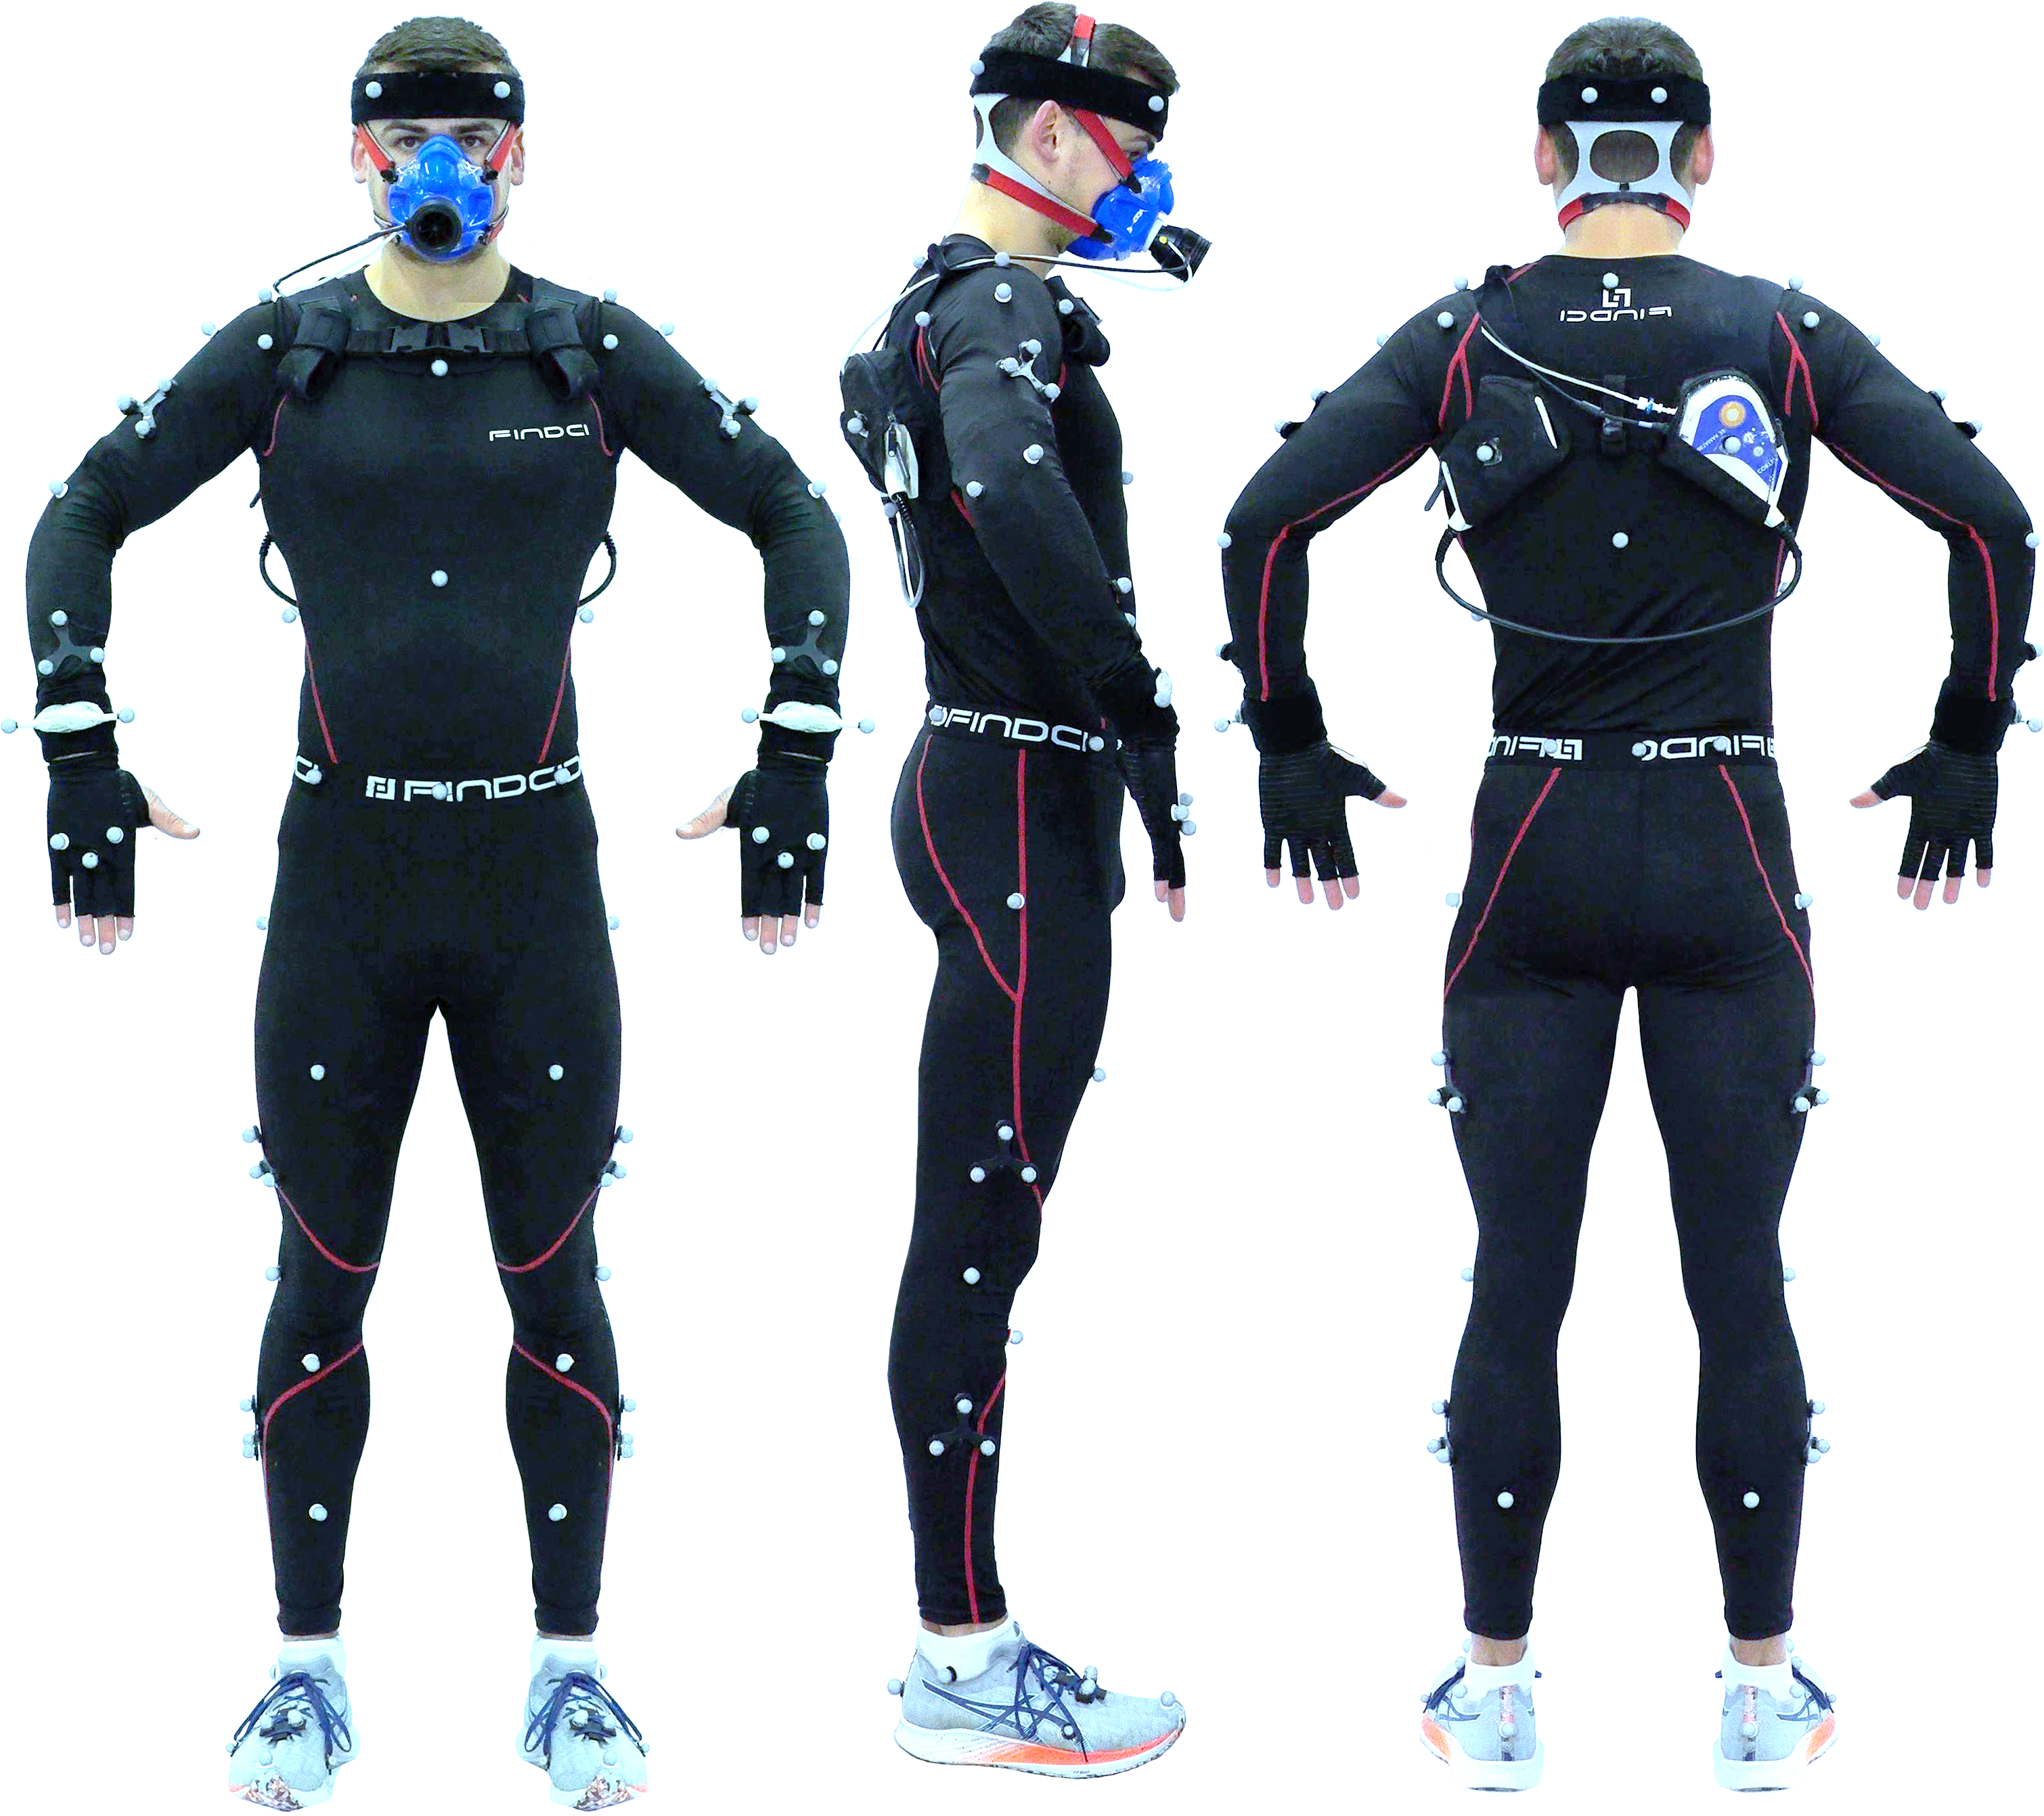
\includegraphics{images/Marker.png}

}

\caption{\label{fig-Marker}Darstellung der Markerpositionierung nach dem
``Full body modelling with Plug-in Gait''-Protokoll befestigt an
enganliegender Kleidung in Frontal-, Seiten- und Rückansicht. Die
reflektierenden Marker sind an anatomischen Referenzpunkten der
Gelenkachsen platziert, um eine dreidimensionale kinematische
Bewegungsanalyse zu ermöglichen.}

\end{figure}%

\end{tcolorbox}

Die 3D-Bewegungsdaten wurden mit 100 Hz aufgezeichnet, was bei 1000
Frames pro Durchgang eine präzise Erfassung der Positionskoordinaten
ermöglichte. Für die Transformation der 3D-Bewegungsdaten in ein
2D-Modell wurden ausschließlich die linksseitigen Marker (L-Präfix) als
Referenzpunkt verwendet. Die ursprünglichen Positionsdaten wurden von
Millimeter in Meter konvertiert und relativ zur Kurbelachse als neuem
Koordinatenursprung transformiert. Folgende Markerpositionen wurden
bestimmt:

\begin{itemize}
\tightlist
\item
  Anatomische Referenzpunkte:

  \begin{itemize}
  \tightlist
  \item
    Kopf (LFHD - Left Front Head, LBHD - Left Back Head): Anteriore und
    posteriore Kopfposition
  \item
    Nackenpunkt (C7): Marker am 7. Halswirbel
  \item
    LSJC (Left Shoulder Joint Center): Zentrum des Schultergelenks
  \item
    LWJC (Left Wrist Joint Center): Zentrum des Handgelenks
  \item
    Becken (LASI - Left Anterior Superior Iliac, LPSI - Left Posterior
    Superior Iliac): Vorderer und hinterer Beckenkamm
  \item
    LHJC (Left Hip Joint Center): Zentrum des Hüftgelenks
  \item
    LKJC (Left Knee Joint Center): Zentrum des Kniegelenks
  \item
    LAJC (Left Ankle Joint Center): Zentrum des Sprunggelenks
  \item
    LToe (Left Toe): Zehenmarker
  \end{itemize}
\item
  Berechnete Bezugspunkte:

  \begin{itemize}
  \tightlist
  \item
    Kopfmittelpunkt (aus LFHD und LBHD): Mittelpunkt zwischen anteriorem
    und posteriorem Kopfmarker
  \item
    Hüftmittelpunkt (aus LASI und LPSI): Mittelpunkt zwischen vorderem
    und hinterem Beckenkammmarker
  \end{itemize}
\end{itemize}

\paragraph{2D-Simulationsmodelle auf Basis der Kinematik
Daten}\label{d-simulationsmodelle-auf-basis-der-kinematik-daten}

Abbildung~\ref{fig-Kinematik_Simulationsmodell_Sitzen} und
Abbildung~\ref{fig-Kinematik_Simulationsmodell_Stehen} präsentieren die
entwickelten 2D-Kinematik-Simulationsmodelle für das Radfahren im Sitzen
und Stehen. Sie zeigen alle erfassten anatomischen Markerpunkte und
berechneten Gelenkzentren, wobei die Kurbelposition sowohl automatisch
als auch manuell angepasst werden kann.

\begin{figure}

\centering{

\includegraphics[width=6.41667in,height=7.21875in]{images/Modell_Kinematik_sitzen_full.html}

}

\caption{\label{fig-Kinematik_Simulationsmodell_Sitzen}2D-Simulationsmodell
im Sitzen anhand der Kinematik Daten.}

\end{figure}%

\begin{figure}

\centering{

\includegraphics[width=6.41667in,height=7.21875in]{images/Modell_Kinematik_stehen_full.html}

}

\caption{\label{fig-Kinematik_Simulationsmodell_Stehen}2D-Simulationsmodell
im Stehen anhand der Kinematik Daten.}

\end{figure}%

\paragraph{\texorpdfstring{2D-Simulationsmodelle auf Basis der Kinematik
Daten zur Berechnung von
P\textsubscript{Int,Kinematik}}{2D-Simulationsmodelle auf Basis der Kinematik Daten zur Berechnung von PInt,Kinematik}}\label{d-simulationsmodelle-auf-basis-der-kinematik-daten-zur-berechnung-von-pintkinematik}

Abbildung~\ref{fig-Kinematik_Simulationsmodell_Sitzen_PInt} und
Abbildung~\ref{fig-Kinematik_Simulationsmodell_Stehen_PInt} zeigen die
für die Berechnung von P\textsubscript{Int,Kinematik} relevanten
Gelenkpunkte und Segmentschwerpunkte des Ober- und Unterschenkelsegments
in beiden Fahrpositionen.

\begin{figure}

\centering{

\includegraphics[width=5.20833in,height=7.5in]{images/Modell_Kinematik_sitzen.html}

}

\caption{\label{fig-Kinematik_Simulationsmodell_Sitzen_PInt}2D-Simulationsmodell
im Sitzen anhand der Kinematik Daten für die Berechnung von
P\textsubscript{Int}.}

\end{figure}%

\begin{figure}

\centering{

\includegraphics[width=5.20833in,height=7.5in]{images/Modell_Kinematik_stehen.html}

}

\caption{\label{fig-Kinematik_Simulationsmodell_Stehen_PInt}2D-Simulationsmodell
im Stehen anhand der Kinematik Daten für die Berechnung von
P\textsubscript{Int}.}

\end{figure}%

Von den erfassten Kinematik-Daten der neun Probanden konnten nur vier
Datensätze für die weitere Analyse verwendet werden, da nur diese die
erforderliche Qualität über mindestens vier Belastungsstufen aufwiesen.
Für die Berechnung der inneren Leistung wurden dabei ausschließlich die
Marker verwendet, die den Modellpunkten P\textsubscript{1} (LToe),
P\textsubscript{2} (LKJC) und P\textsubscript{3} (LHJC) entsprachen,
während die übrigen erfassten Punkte in diesem Modell nur der
Visualisierung der gesamten Tretbewegung dienten. Die Quantifizierung
der inneren Arbeit anhand der kinematischen Messdaten erfolgte analog
zur Berechnung der P\textsubscript{Int,Modell} des Simulationsmodells.
Dabei wurden die real erfassten Koordinaten von LToe, LKJC und LHJC für
die Modellpunkte P\textsubscript{1}, P\textsubscript{2} und
P\textsubscript{3} anstelle der modellierten Gelenkpositionen verwendet.
Die resultierende innere Leistung, die sich aus den berechneten
kinematischen Daten ableitet, wird in der vorliegenden Untersuchung als
P\textsubscript{Int,Kinematik} bezeichnet.

\paragraph{Exemplarische Verläufe der inneren Leistung, berechnet aus
kinematischen
Messdaten}\label{exemplarische-verluxe4ufe-der-inneren-leistung-berechnet-aus-kinematischen-messdaten}

\paragraph{Sitzen}

\begin{figure}

\centering{

\includegraphics{Innere_Arbeit_files/figure-pdf/fig-PInt_Kinematik_19_5-1.pdf}

}

\caption{\label{fig-PInt_Kinematik_19_5}Zeitlicher Verlauf der aus der
3D-Kinematik berechneten positiven Anteile der inneren Leistung
(P\textsubscript{int}) beider Beine mit gemitteltem
P\textsubscript{int}-Wert (grau gestrichelt) für 19\_5.}

\end{figure}%

\paragraph{Stehen}

\begin{figure}

\centering{

\includegraphics{Innere_Arbeit_files/figure-pdf/fig-PInt_Kinematik_19_6-1.pdf}

}

\caption{\label{fig-PInt_Kinematik_19_6}Zeitlicher Verlauf der aus der
3D-Kinematik berechneten positiven Anteile der inneren Leistung
(P\textsubscript{int}) beider Beine mit gemitteltem
P\textsubscript{int}-Wert (grau gestrichelt) für 19\_6.}

\end{figure}%

Basierend auf diesen Berechnungen wurde ein methodischer Ansatz
entwickelt, um die innere Leistung auch für Probanden zu approximieren,
für die keine validen Kinematikdaten vorlagen. Hierzu wurde zunächst die
systematische Abweichung zwischen P\textsubscript{Int,Kinematik} und
P\textsubscript{Int,Modell} für beide Bedingungen quantifiziert
(Gleichung~\ref{eq-PInt_Diff}):

\begin{equation}\phantomsection\label{eq-PInt_Diff}{
P_{Int,Diff} = 
\begin{cases} 
P_{Int,Kinematik,stehen} - P_{Int,Modell,stehen} & \text{für Bedingung = "stehen"} \\
P_{Int,Kinematik,sitzen} - P_{Int,Modell,sitzen} & \text{für Bedingung = "sitzen"}
\end{cases}
}\end{equation}

Die mittleren Differenzen zwischen P\textsubscript{Int,Kinematik} und
P\textsubscript{Int,Modell} wurden separat für die Bedingungen
``stehen'' und ``sitzen'' ermittelt. Diese systematischen Differenzen
dienten als Grundlage für die Modellierung von
P\textsubscript{Int,Kinematik,Modell} gemäß
Gleichung~\ref{eq-PInt_Kinematik_Modell}:

\begin{equation}\phantomsection\label{eq-PInt_Kinematik_Modell}{
P_{Int,Kinematik,Modell} = 
\begin{cases} 
P_{Int,Modell} + P_{Int,Diff,stehen} & \text{für Bedingung "stehen"} \\
P_{Int,Modell} + P_{Int,Diff,sitzen} & \text{für Bedingung "sitzen"}
\end{cases}
}\end{equation}

Dieser Ansatz ermöglichte die Generierung vergleichbarer
P\textsubscript{Int,Kinematik,Modell}-Werte für sämtliche Probanden und
Bedingungen, auch in Abwesenheit direkter kinematischer Messdaten.

\subparagraph{\texorpdfstring{\textbf{\emph{R-Code zur Berechnung der
Inneren Arbeit auf Basis realer
Kinematikdaten}}}{R-Code zur Berechnung der Inneren Arbeit auf Basis realer Kinematikdaten}}\label{r-code-zur-berechnung-der-inneren-arbeit-auf-basis-realer-kinematikdaten}

\emph{Der folgende Code implementiert die Berechnung der inneren Arbeit
anhand der experimentell erfassten Kinematikdaten. Basierend auf den
räumlichen Koordinaten der Gelenkpunkte (Hüfte, Knie, Sprunggelenk)
werden die Segmentwinkel, Schwerpunktgeschwindigkeiten und kinetischen
Energien bestimmt. Die zeitlichen Änderungen der kinetischen Energien
ergeben die innere Leistung. Durch die Analyse der Zyklen wird die
innere Arbeit für beide Beine separat ermittelt.}

\begin{Shaded}
\begin{Highlighting}[]
\DocumentationTok{\#\#\#\#\#\# Konstanten und Parameter \#\#\#\#\#\#}
\CommentTok{\# Basisdaten aus Erg\_data\_df}
\NormalTok{Masse }\OtherTok{\textless{}{-}}\NormalTok{ Erg\_data\_df[Erg\_data\_df}\SpecialCharTok{$}\NormalTok{Name }\SpecialCharTok{==}\NormalTok{ name, }\StringTok{"Masse"}\NormalTok{]}
\NormalTok{uOS }\OtherTok{\textless{}{-}}\NormalTok{ Erg\_data\_df[Erg\_data\_df}\SpecialCharTok{$}\NormalTok{Name }\SpecialCharTok{==}\NormalTok{ name, }\StringTok{"uOS"}\NormalTok{]}
\NormalTok{uUS }\OtherTok{\textless{}{-}}\NormalTok{ Erg\_data\_df[Erg\_data\_df}\SpecialCharTok{$}\NormalTok{Name }\SpecialCharTok{==}\NormalTok{ name, }\StringTok{"uUS"}\NormalTok{]}
\NormalTok{lBein }\OtherTok{\textless{}{-}}\NormalTok{ Erg\_data\_df[Erg\_data\_df}\SpecialCharTok{$}\NormalTok{Name }\SpecialCharTok{==}\NormalTok{ name, }\StringTok{"lBein"}\NormalTok{]}

\CommentTok{\# Geometrische Konstanten}
\NormalTok{Faktor }\OtherTok{\textless{}{-}} \FloatTok{1.0}
\NormalTok{S }\OtherTok{\textless{}{-}}\NormalTok{ lBein }\SpecialCharTok{*} \FloatTok{0.883} \SpecialCharTok{*}\NormalTok{ Faktor }\CommentTok{\# Abstand vom Hüftgelenk zur Kurbelachse {-} Lemond Methode}

\CommentTok{\# Segmentmassen und {-}eigenschaften}
\NormalTok{rRelOS }\OtherTok{\textless{}{-}} \FloatTok{0.1416} \CommentTok{\# relative Segmentmasse OS}
\NormalTok{rRelUS }\OtherTok{\textless{}{-}} \FloatTok{0.0433} \CommentTok{\# relative Segmentmasse US}
\NormalTok{lambdaOS }\OtherTok{\textless{}{-}} \FloatTok{0.4095} \CommentTok{\# Abstand proximaler Punkt OS {-} Schwerpunkt}
\NormalTok{lambdaUS }\OtherTok{\textless{}{-}} \FloatTok{0.4459} \CommentTok{\# Abstand proximaler Punkt US {-} Schwerpunkt}
\NormalTok{mOS }\OtherTok{\textless{}{-}}\NormalTok{ Masse }\SpecialCharTok{*}\NormalTok{ rRelOS }\CommentTok{\# Segmentmasse OS}
\NormalTok{mUS }\OtherTok{\textless{}{-}}\NormalTok{ Masse }\SpecialCharTok{*}\NormalTok{ rRelUS }\CommentTok{\# Segmentmasse US}
\NormalTok{thetaKurbel }\OtherTok{\textless{}{-}} \FloatTok{0.002} \CommentTok{\# Trägheitsmoment der Fahrradkurbel [kg m\^{}2]}

\DocumentationTok{\#\#\#\#\#\# Hauptberechnungen im DataFrame \#\#\#\#\#\#}
\NormalTok{df }\OtherTok{\textless{}{-}}\NormalTok{ df }\SpecialCharTok{\%\textgreater{}\%}
  \FunctionTok{mutate}\NormalTok{(}
    \CommentTok{\# Winkel{-} und Zeitberechnungen}
    \AttributeTok{phi1 =} \FunctionTok{ifelse}\NormalTok{(}\FunctionTok{atan2}\NormalTok{(P1y, P1x) }\SpecialCharTok{\textless{}} \DecValTok{0}\NormalTok{, }\FunctionTok{atan2}\NormalTok{(P1y, P1x) }\SpecialCharTok{+} \DecValTok{2} \SpecialCharTok{*}\NormalTok{ pi, }\FunctionTok{atan2}\NormalTok{(P1y, P1x)),}
    \AttributeTok{Grad =}\NormalTok{ phi1 }\SpecialCharTok{*}\NormalTok{ (}\DecValTok{180} \SpecialCharTok{/}\NormalTok{ pi),}
    \AttributeTok{delta\_t =} \DecValTok{1} \SpecialCharTok{/} \DecValTok{100}\NormalTok{,}
    \AttributeTok{delta\_phi1 =} \FunctionTok{corrected\_delta\_phi1}\NormalTok{(phi1),}
    \AttributeTok{omega =}\NormalTok{ delta\_phi1 }\SpecialCharTok{/}\NormalTok{ delta\_t,}
    \AttributeTok{nD =}\NormalTok{ omega }\SpecialCharTok{/}\NormalTok{ (}\DecValTok{2} \SpecialCharTok{*}\NormalTok{ pi) }\SpecialCharTok{*} \DecValTok{60}\NormalTok{,}
    \AttributeTok{nD\_avg =} \FunctionTok{mean}\NormalTok{(omega, }\AttributeTok{na.rm =} \ConstantTok{TRUE}\NormalTok{) }\SpecialCharTok{/}\NormalTok{ (}\DecValTok{2} \SpecialCharTok{*}\NormalTok{ pi) }\SpecialCharTok{*} \DecValTok{60}\NormalTok{,}
    \AttributeTok{T =} \DecValTok{60} \SpecialCharTok{/}\NormalTok{ nD,}
    
    \CommentTok{\# Längenberechnungen}
    \AttributeTok{lOS =} \FunctionTok{sqrt}\NormalTok{((P3x}\SpecialCharTok{{-}}\NormalTok{P2x)}\SpecialCharTok{\^{}}\DecValTok{2}\SpecialCharTok{+}\NormalTok{(P3y}\SpecialCharTok{{-}}\NormalTok{P2y)}\SpecialCharTok{\^{}}\DecValTok{2}\NormalTok{),}
    \AttributeTok{lUS =} \FunctionTok{sqrt}\NormalTok{((P2x}\SpecialCharTok{{-}}\NormalTok{LAJC\_X)}\SpecialCharTok{\^{}}\DecValTok{2}\SpecialCharTok{+}\NormalTok{(P2y}\SpecialCharTok{{-}}\NormalTok{LAJC\_Y)}\SpecialCharTok{\^{}}\DecValTok{2}\NormalTok{),}
    \AttributeTok{lOS\_avg =} \FunctionTok{mean}\NormalTok{(lOS),}
    \AttributeTok{lUS\_avg =} \FunctionTok{mean}\NormalTok{(lUS),}
    
    \CommentTok{\# Trägheitsmomente}
    \AttributeTok{thetaOS =}\NormalTok{ (}\DecValTok{1}\SpecialCharTok{/}\DecValTok{4}\NormalTok{) }\SpecialCharTok{*}\NormalTok{ mOS }\SpecialCharTok{*}\NormalTok{ (uOS }\SpecialCharTok{/}\NormalTok{ (}\DecValTok{2} \SpecialCharTok{*}\NormalTok{ pi))}\SpecialCharTok{\^{}}\DecValTok{2} \SpecialCharTok{+}\NormalTok{ (}\DecValTok{1}\SpecialCharTok{/}\DecValTok{12}\NormalTok{) }\SpecialCharTok{*}\NormalTok{ mOS }\SpecialCharTok{*}\NormalTok{ lOS\_avg}\SpecialCharTok{\^{}}\DecValTok{2}\NormalTok{,}
    \AttributeTok{thetaUS =}\NormalTok{ (}\DecValTok{1}\SpecialCharTok{/}\DecValTok{4}\NormalTok{) }\SpecialCharTok{*}\NormalTok{ mUS }\SpecialCharTok{*}\NormalTok{ (uUS }\SpecialCharTok{/}\NormalTok{ (}\DecValTok{2} \SpecialCharTok{*}\NormalTok{ pi))}\SpecialCharTok{\^{}}\DecValTok{2} \SpecialCharTok{+}\NormalTok{ (}\DecValTok{1}\SpecialCharTok{/}\DecValTok{12}\NormalTok{) }\SpecialCharTok{*}\NormalTok{ mUS }\SpecialCharTok{*}\NormalTok{ lUS\_avg}\SpecialCharTok{\^{}}\DecValTok{2}\NormalTok{,}
    
    \CommentTok{\# Schwerpunktberechnungen}
    \AttributeTok{SpOS\_X =}\NormalTok{ P3x }\SpecialCharTok{{-}}\NormalTok{ lambdaOS }\SpecialCharTok{*}\NormalTok{ (P3x}\SpecialCharTok{{-}}\NormalTok{P2x),}
    \AttributeTok{SpOS\_Y =}\NormalTok{ P3y }\SpecialCharTok{{-}}\NormalTok{ lambdaOS }\SpecialCharTok{*}\NormalTok{ (P3y}\SpecialCharTok{{-}}\NormalTok{P2y),}
    \AttributeTok{SpUS\_X =}\NormalTok{ P2x }\SpecialCharTok{{-}}\NormalTok{ lambdaOS }\SpecialCharTok{*}\NormalTok{ (P2x}\SpecialCharTok{{-}}\NormalTok{LAJC\_X),}
    \AttributeTok{SpUS\_Y =}\NormalTok{ P2y }\SpecialCharTok{{-}}\NormalTok{ lambdaOS }\SpecialCharTok{*}\NormalTok{ (P2y}\SpecialCharTok{{-}}\NormalTok{LAJC\_Y),}
    
    \CommentTok{\# Geschwindigkeitsberechnungen}
    \AttributeTok{d\_SpOS =} \FunctionTok{sqrt}\NormalTok{((}\FunctionTok{lead}\NormalTok{(SpOS\_X) }\SpecialCharTok{{-}}\NormalTok{ SpOS\_X)}\SpecialCharTok{\^{}}\DecValTok{2} \SpecialCharTok{+}\NormalTok{ (}\FunctionTok{lead}\NormalTok{(SpOS\_Y) }\SpecialCharTok{{-}}\NormalTok{ SpOS\_Y)}\SpecialCharTok{\^{}}\DecValTok{2}\NormalTok{),}
    \AttributeTok{d\_SpUS =} \FunctionTok{sqrt}\NormalTok{((}\FunctionTok{lead}\NormalTok{(SpUS\_X) }\SpecialCharTok{{-}}\NormalTok{ SpUS\_X)}\SpecialCharTok{\^{}}\DecValTok{2} \SpecialCharTok{+}\NormalTok{ (}\FunctionTok{lead}\NormalTok{(SpUS\_Y) }\SpecialCharTok{{-}}\NormalTok{ SpUS\_Y)}\SpecialCharTok{\^{}}\DecValTok{2}\NormalTok{),}
    \AttributeTok{v\_SpOS =} \FunctionTok{ifelse}\NormalTok{(}\FunctionTok{is.na}\NormalTok{(d\_SpOS), }\ConstantTok{NA}\NormalTok{, d\_SpOS }\SpecialCharTok{/}\NormalTok{ delta\_t),}
    \AttributeTok{v\_SpUS =} \FunctionTok{ifelse}\NormalTok{(}\FunctionTok{is.na}\NormalTok{(d\_SpUS), }\ConstantTok{NA}\NormalTok{, d\_SpUS }\SpecialCharTok{/}\NormalTok{ delta\_t),}
    
    \CommentTok{\# Winkelberechnungen}
    \AttributeTok{phi2 =} \FunctionTok{acos}\NormalTok{((P2x}\SpecialCharTok{{-}}\NormalTok{P1x) }\SpecialCharTok{/}\NormalTok{ lUS),}
    \AttributeTok{phi3 =} \FunctionTok{acos}\NormalTok{((P3x}\SpecialCharTok{{-}}\NormalTok{P2x) }\SpecialCharTok{/}\NormalTok{ lOS),}
    \AttributeTok{omega\_SpOS =}\NormalTok{ (}\FunctionTok{lead}\NormalTok{(phi2) }\SpecialCharTok{{-}}\NormalTok{ phi2) }\SpecialCharTok{/}\NormalTok{ delta\_t,}
    \AttributeTok{omega\_SpUS =}\NormalTok{ (}\FunctionTok{lead}\NormalTok{(phi3) }\SpecialCharTok{{-}}\NormalTok{ phi3) }\SpecialCharTok{/}\NormalTok{ delta\_t,}
    \AttributeTok{omega\_Kurbel =}\NormalTok{ (}\FunctionTok{lead}\NormalTok{(phi2) }\SpecialCharTok{{-}}\NormalTok{ phi2) }\SpecialCharTok{/}\NormalTok{ delta\_t,}
    
    \CommentTok{\# Energieberechnungen}
    \AttributeTok{Ekin\_rot =} \FloatTok{0.5} \SpecialCharTok{*}\NormalTok{ (thetaOS }\SpecialCharTok{*}\NormalTok{ omega\_SpOS}\SpecialCharTok{\^{}}\DecValTok{2} \SpecialCharTok{+}\NormalTok{ thetaUS }\SpecialCharTok{*}\NormalTok{ omega\_SpUS}\SpecialCharTok{\^{}}\DecValTok{2} \SpecialCharTok{+}\NormalTok{ thetaKurbel }\SpecialCharTok{*}\NormalTok{ omega\_Kurbel}\SpecialCharTok{\^{}}\DecValTok{2}\NormalTok{),}
    \AttributeTok{Ekin\_trans =} \FloatTok{0.5} \SpecialCharTok{*}\NormalTok{ (mOS }\SpecialCharTok{*}\NormalTok{ v\_SpOS}\SpecialCharTok{\^{}}\DecValTok{2} \SpecialCharTok{+}\NormalTok{ mUS }\SpecialCharTok{*}\NormalTok{ v\_SpUS}\SpecialCharTok{\^{}}\DecValTok{2}\NormalTok{),}
    \AttributeTok{delta\_Ekin\_rot =} \FunctionTok{lead}\NormalTok{(Ekin\_rot) }\SpecialCharTok{{-}}\NormalTok{ Ekin\_rot,}
    \AttributeTok{delta\_Ekin\_trans =} \FunctionTok{lead}\NormalTok{(Ekin\_trans) }\SpecialCharTok{{-}}\NormalTok{ Ekin\_trans,}
    \AttributeTok{delta\_Ekin\_ges =}\NormalTok{ delta\_Ekin\_rot }\SpecialCharTok{+}\NormalTok{ delta\_Ekin\_trans,}
    \AttributeTok{PInt\_Rechts =}\NormalTok{ delta\_Ekin\_ges }\SpecialCharTok{/}\NormalTok{ delta\_t}
\NormalTok{  ) }\SpecialCharTok{\%\textgreater{}\%}
  \FunctionTok{slice}\NormalTok{(}\DecValTok{1}\SpecialCharTok{:}\NormalTok{(}\FunctionTok{n}\NormalTok{() }\SpecialCharTok{{-}} \DecValTok{2}\NormalTok{)) }\SpecialCharTok{\%\textgreater{}\%}
  \FunctionTok{select}\NormalTok{(Frame, Grad, phi1, delta\_phi1, omega, T, nD, nD\_avg, Masse, }\FunctionTok{everything}\NormalTok{())}

\DocumentationTok{\#\#\#\#\#\# Ausreißerbehandlung \#\#\#\#\#\#}
\CommentTok{\# Ausreißergrenzen bestimmen}
\NormalTok{Q1 }\OtherTok{\textless{}{-}} \FunctionTok{quantile}\NormalTok{(df}\SpecialCharTok{$}\NormalTok{PInt\_Rechts, }\FloatTok{0.25}\NormalTok{, }\AttributeTok{na.rm =} \ConstantTok{TRUE}\NormalTok{)}
\NormalTok{Q3 }\OtherTok{\textless{}{-}} \FunctionTok{quantile}\NormalTok{(df}\SpecialCharTok{$}\NormalTok{PInt\_Rechts, }\FloatTok{0.75}\NormalTok{, }\AttributeTok{na.rm =} \ConstantTok{TRUE}\NormalTok{)}
\NormalTok{IQR }\OtherTok{\textless{}{-}}\NormalTok{ Q3 }\SpecialCharTok{{-}}\NormalTok{ Q1}
\NormalTok{lower\_bound }\OtherTok{\textless{}{-}}\NormalTok{ Q1 }\SpecialCharTok{{-}} \FloatTok{1.5} \SpecialCharTok{*}\NormalTok{ IQR}
\NormalTok{upper\_bound }\OtherTok{\textless{}{-}}\NormalTok{ Q3 }\SpecialCharTok{+} \FloatTok{1.5} \SpecialCharTok{*}\NormalTok{ IQR}

\CommentTok{\# Ausreißer ersetzen}
\NormalTok{df}\SpecialCharTok{$}\NormalTok{PInt\_Rechts }\OtherTok{\textless{}{-}} \FunctionTok{ifelse}\NormalTok{(df}\SpecialCharTok{$}\NormalTok{PInt\_Rechts }\SpecialCharTok{\textless{}}\NormalTok{ lower\_bound }\SpecialCharTok{|}\NormalTok{ df}\SpecialCharTok{$}\NormalTok{PInt\_Rechts }\SpecialCharTok{\textgreater{}}\NormalTok{ upper\_bound, }\ConstantTok{NA}\NormalTok{, df}\SpecialCharTok{$}\NormalTok{PInt\_Rechts)}

\DocumentationTok{\#\#\#\#\#\# Imputation fehlender Werte \#\#\#\#\#\#}
\NormalTok{df}\SpecialCharTok{$}\NormalTok{PInt\_Rechts\_imputed }\OtherTok{\textless{}{-}}\NormalTok{ df}\SpecialCharTok{$}\NormalTok{PInt\_Rechts}
\ControlFlowTok{for}\NormalTok{ (i }\ControlFlowTok{in} \DecValTok{1}\SpecialCharTok{:}\FunctionTok{length}\NormalTok{(df}\SpecialCharTok{$}\NormalTok{PInt\_Rechts\_imputed)) \{}
  \ControlFlowTok{if}\NormalTok{ (}\FunctionTok{is.na}\NormalTok{(df}\SpecialCharTok{$}\NormalTok{PInt\_Rechts\_imputed[i])) \{}
\NormalTok{    valid\_indices\_above }\OtherTok{\textless{}{-}} \FunctionTok{which}\NormalTok{(}\SpecialCharTok{!}\FunctionTok{is.na}\NormalTok{(df}\SpecialCharTok{$}\NormalTok{PInt\_Rechts\_imputed[i}\SpecialCharTok{:}\FunctionTok{min}\NormalTok{(i}\SpecialCharTok{+}\DecValTok{2}\NormalTok{, }\FunctionTok{nrow}\NormalTok{(df))]))}
\NormalTok{    valid\_indices\_below }\OtherTok{\textless{}{-}} \FunctionTok{which}\NormalTok{(}\SpecialCharTok{!}\FunctionTok{is.na}\NormalTok{(df}\SpecialCharTok{$}\NormalTok{PInt\_Rechts\_imputed[}\FunctionTok{max}\NormalTok{(i}\DecValTok{{-}2}\NormalTok{, }\DecValTok{1}\NormalTok{)}\SpecialCharTok{:}\NormalTok{i]))}
    
    \ControlFlowTok{if}\NormalTok{ (}\FunctionTok{length}\NormalTok{(valid\_indices\_above) }\SpecialCharTok{\textgreater{}} \DecValTok{0} \SpecialCharTok{\&\&} \FunctionTok{length}\NormalTok{(valid\_indices\_below) }\SpecialCharTok{\textgreater{}} \DecValTok{0}\NormalTok{) \{}
\NormalTok{      upper\_mean }\OtherTok{\textless{}{-}} \FunctionTok{mean}\NormalTok{(df}\SpecialCharTok{$}\NormalTok{PInt\_Rechts\_imputed[i }\SpecialCharTok{+}\NormalTok{ valid\_indices\_above], }\AttributeTok{na.rm =} \ConstantTok{TRUE}\NormalTok{)}
\NormalTok{      lower\_mean }\OtherTok{\textless{}{-}} \FunctionTok{mean}\NormalTok{(df}\SpecialCharTok{$}\NormalTok{PInt\_Rechts\_imputed[i }\SpecialCharTok{{-}}\NormalTok{ valid\_indices\_below], }\AttributeTok{na.rm =} \ConstantTok{TRUE}\NormalTok{)}
\NormalTok{      df}\SpecialCharTok{$}\NormalTok{PInt\_Rechts\_imputed[i] }\OtherTok{\textless{}{-}} \FunctionTok{mean}\NormalTok{(}\FunctionTok{c}\NormalTok{(upper\_mean, lower\_mean), }\AttributeTok{na.rm =} \ConstantTok{TRUE}\NormalTok{)}
\NormalTok{    \} }\ControlFlowTok{else} \ControlFlowTok{if}\NormalTok{ (}\FunctionTok{length}\NormalTok{(valid\_indices\_above) }\SpecialCharTok{\textgreater{}} \DecValTok{0}\NormalTok{) \{}
\NormalTok{      df}\SpecialCharTok{$}\NormalTok{PInt\_Rechts\_imputed[i] }\OtherTok{\textless{}{-}} \FunctionTok{mean}\NormalTok{(df}\SpecialCharTok{$}\NormalTok{PInt\_Rechts\_imputed[i }\SpecialCharTok{+}\NormalTok{ valid\_indices\_above], }\AttributeTok{na.rm =} \ConstantTok{TRUE}\NormalTok{)}
\NormalTok{    \} }\ControlFlowTok{else} \ControlFlowTok{if}\NormalTok{ (}\FunctionTok{length}\NormalTok{(valid\_indices\_below) }\SpecialCharTok{\textgreater{}} \DecValTok{0}\NormalTok{) \{}
\NormalTok{      df}\SpecialCharTok{$}\NormalTok{PInt\_Rechts\_imputed[i] }\OtherTok{\textless{}{-}} \FunctionTok{mean}\NormalTok{(df}\SpecialCharTok{$}\NormalTok{PInt\_Rechts\_imputed[i }\SpecialCharTok{{-}}\NormalTok{ valid\_indices\_below], }\AttributeTok{na.rm =} \ConstantTok{TRUE}\NormalTok{)}
\NormalTok{    \}}
\NormalTok{  \}}
\NormalTok{\}}
\NormalTok{df}\SpecialCharTok{$}\NormalTok{PInt\_Rechts }\OtherTok{\textless{}{-}}\NormalTok{ df}\SpecialCharTok{$}\NormalTok{PInt\_Rechts\_imputed}
\NormalTok{df}\SpecialCharTok{$}\NormalTok{PInt\_Rechts\_imputed }\OtherTok{\textless{}{-}} \ConstantTok{NULL}

\DocumentationTok{\#\#\#\#\#\# Zyklusanalyse \#\#\#\#\#\#}
\CommentTok{\# Zyklusparameter}
\NormalTok{Startwert\_Grad }\OtherTok{\textless{}{-}}\NormalTok{ df}\SpecialCharTok{$}\NormalTok{Grad[}\DecValTok{1}\NormalTok{]}
\NormalTok{Toleranz }\OtherTok{\textless{}{-}} \DecValTok{3}

\CommentTok{\# Zyklusendpunkte finden}
\NormalTok{Ende\_Zyklus\_Indizes }\OtherTok{\textless{}{-}} \FunctionTok{which}\NormalTok{(}\FunctionTok{abs}\NormalTok{(df}\SpecialCharTok{$}\NormalTok{Grad }\SpecialCharTok{{-}}\NormalTok{ Startwert\_Grad) }\SpecialCharTok{\textless{}=}\NormalTok{ Toleranz)}
\NormalTok{diff\_Ende\_Zyklus\_Indizes }\OtherTok{\textless{}{-}} \FunctionTok{c}\NormalTok{(}\FunctionTok{diff}\NormalTok{(Ende\_Zyklus\_Indizes), Toleranz }\SpecialCharTok{+} \DecValTok{1}\NormalTok{)}
\NormalTok{gefilterte\_Indizes }\OtherTok{\textless{}{-}}\NormalTok{ Ende\_Zyklus\_Indizes[diff\_Ende\_Zyklus\_Indizes }\SpecialCharTok{\textgreater{}} \DecValTok{1}\NormalTok{]}
\NormalTok{Anzahl\_Zyklen }\OtherTok{\textless{}{-}} \FunctionTok{length}\NormalTok{(gefilterte\_Indizes)}\SpecialCharTok{{-}}\DecValTok{1}
\NormalTok{Ende\_Zyklen }\OtherTok{\textless{}{-}}\NormalTok{ gefilterte\_Indizes[}\FunctionTok{length}\NormalTok{(gefilterte\_Indizes)]}

\CommentTok{\# DataFrame auf komplette Zyklen beschränken}
\NormalTok{df }\OtherTok{\textless{}{-}}\NormalTok{ df[}\DecValTok{1}\SpecialCharTok{:}\NormalTok{Ende\_Zyklen, ]}
\NormalTok{Laenge\_Zyklus }\OtherTok{\textless{}{-}} \FunctionTok{round}\NormalTok{(}\FunctionTok{length}\NormalTok{(df}\SpecialCharTok{$}\NormalTok{Grad) }\SpecialCharTok{/}\NormalTok{ Anzahl\_Zyklen, }\DecValTok{0}\NormalTok{)}

\DocumentationTok{\#\#\#\#\#\# Berechnung linkes Bein \#\#\#\#\#\#}
\NormalTok{verschieben }\OtherTok{\textless{}{-}} \FunctionTok{round}\NormalTok{(Laenge\_Zyklus }\SpecialCharTok{*} \FloatTok{0.5}\NormalTok{)}
\NormalTok{verschobene\_Werte }\OtherTok{\textless{}{-}} \FunctionTok{numeric}\NormalTok{(}\FunctionTok{nrow}\NormalTok{(df))}
\ControlFlowTok{for}\NormalTok{ (i }\ControlFlowTok{in} \DecValTok{1}\SpecialCharTok{:}\FunctionTok{nrow}\NormalTok{(df)) \{}
\NormalTok{  index\_in\_PInt\_Rechts }\OtherTok{\textless{}{-}}\NormalTok{ ((i }\SpecialCharTok{+}\NormalTok{ verschieben }\SpecialCharTok{{-}} \DecValTok{1}\NormalTok{) }\SpecialCharTok{\%\%} \FunctionTok{nrow}\NormalTok{(df)) }\SpecialCharTok{+} \DecValTok{1}
\NormalTok{  verschobene\_Werte[i] }\OtherTok{\textless{}{-}}\NormalTok{ df}\SpecialCharTok{$}\NormalTok{PInt\_Rechts[index\_in\_PInt\_Rechts]}
\NormalTok{\}}

\DocumentationTok{\#\#\#\#\#\# Finale Berechnungen und Glättung \#\#\#\#\#\#}
\NormalTok{fensterbreite }\OtherTok{\textless{}{-}} \DecValTok{15}
\NormalTok{df }\OtherTok{\textless{}{-}}\NormalTok{ df }\SpecialCharTok{\%\textgreater{}\%}
  \FunctionTok{mutate}\NormalTok{(}
    \AttributeTok{PInt\_Links =}\NormalTok{ verschobene\_Werte,}
    \AttributeTok{PInt\_Links\_Positiv =} \FunctionTok{ifelse}\NormalTok{(PInt\_Links }\SpecialCharTok{\textless{}} \DecValTok{0}\NormalTok{, }\DecValTok{0}\NormalTok{, PInt\_Links),}
    \AttributeTok{PInt\_Rechts\_Positiv =} \FunctionTok{ifelse}\NormalTok{(PInt\_Rechts }\SpecialCharTok{\textless{}} \DecValTok{0}\NormalTok{, }\DecValTok{0}\NormalTok{, PInt\_Rechts),}
    \AttributeTok{PInt\_Kinematik =} \FunctionTok{mean}\NormalTok{(PInt\_Rechts\_Positiv, }\AttributeTok{na.rm =} \ConstantTok{TRUE}\NormalTok{) }\SpecialCharTok{+} \FunctionTok{mean}\NormalTok{(PInt\_Links\_Positiv, }\AttributeTok{na.rm =} \ConstantTok{TRUE}\NormalTok{),}
    \AttributeTok{PInt\_Rechts\_smooth =} \FunctionTok{rollmean}\NormalTok{(PInt\_Rechts, fensterbreite, }\AttributeTok{fill =} \ConstantTok{NA}\NormalTok{, }\AttributeTok{align =} \StringTok{"right"}\NormalTok{),}
    \AttributeTok{PInt\_Rechts\_Positiv\_smooth =} \FunctionTok{ifelse}\NormalTok{(PInt\_Rechts\_smooth }\SpecialCharTok{\textless{}} \DecValTok{0}\NormalTok{, }\DecValTok{0}\NormalTok{, PInt\_Rechts\_smooth),}
    \AttributeTok{PInt\_Links\_smooth =} \FunctionTok{rollmean}\NormalTok{(PInt\_Links, fensterbreite, }\AttributeTok{fill =} \ConstantTok{NA}\NormalTok{, }\AttributeTok{align =} \StringTok{"right"}\NormalTok{),}
    \AttributeTok{PInt\_Links\_Positiv\_smooth =} \FunctionTok{ifelse}\NormalTok{(PInt\_Links\_smooth }\SpecialCharTok{\textless{}} \DecValTok{0}\NormalTok{, }\DecValTok{0}\NormalTok{, PInt\_Links\_smooth)}
\NormalTok{  )}

\DocumentationTok{\#\#\#\#\#\# Ergebnisspeicherung \#\#\#\#\#\#}
\NormalTok{PInt\_Kinematik\_list[[name]] }\OtherTok{\textless{}{-}}\NormalTok{ df}
\NormalTok{mean\_nD\_avg }\OtherTok{\textless{}{-}} \FunctionTok{mean}\NormalTok{(df}\SpecialCharTok{$}\NormalTok{nD\_avg, }\AttributeTok{na.rm =} \ConstantTok{TRUE}\NormalTok{)}
\end{Highlighting}
\end{Shaded}

\subsubsection{\texorpdfstring{Explorativ:
W\textsubscript{Int}-Berechnung nach Winter
(1979)}{Explorativ: WInt-Berechnung nach Winter (1979)}}\label{explorativ-wint-berechnung-nach-winter1979}

Die ursprüngliche Berechnung der inneren Arbeit
P\textsubscript{Int,Kinematik,Modell} führte zu differenzierten
Ergebnissen zwischen den beiden Körperpositionen. Während die
Berechnungswerte der sitzenden Position mit den in der Literatur
berichteten Werten übereinstimmten, zeigten sich für die
Belastungsdurchgänge im Stehen physiologisch nicht plausible Ergebnisse.
Eine detaillierte Analyse der Berechnungsergebnisse offenbarte, dass
zwar bei identischer Trittrate minimal höhere
P\textsubscript{Int,Kinematik,Modell}-Werte im Stehen auftraten, jedoch
die systematisch niedrigeren Trittraten bei gleicher
Belastungsintensität zu substantiell geringeren
P\textsubscript{Int}-Werten in der stehenden Position führten. Diese
Diskrepanz steht im Widerspruch zu den berechneten Wirkungsgraden
(η\textsubscript{Total}, η\textsubscript{Netto},
η\textsubscript{Brutto}, alle ohne Berücksichtigung der inneren
Leistung) sowie den erhobenen physiologischen Parametern des
durchschnittlichen Sauerstoffvolumenstroms (\(\dot{V}O_2\)) und der
durchschnittlichen Herzrate. Da diese Parameter bei vergleichbarer
mechanischer Leistung keine signifikanten Unterschiede zwischen
stehender und sitzender Position aufwiesen, lässt sich die Hypothese
ableiten, dass die innere Leistung in beiden Körperpositionen ähnliche
Werte aufweisen sollte. Aufgrund der fehlenden Bestätigung dieser
Annahme durch die gewählten Berechnungsmethoden wurde nachträglich ein
alternativer Berechnungsansatz untersucht. Dieser basiert auf dem Modell
von Winter (1979) und wurde gemäß der Methodik von Hansen et al. (2004)
für die spezifischen Anforderungen des Radfahrens adaptiert. Die
wesentlichen methodischen Erweiterungen gegenüber dem zuvor
beschriebenen Berechnungsweg für P\textsubscript{Int,Kinematik,Modell}
umfassten drei zentrale Aspekte: Erstens die Integration der
potentiellen Energie der Segmente, zweitens die Berücksichtigung des
HAT-Segments (Head-Arms-Trunk) als zusammenhängende biomechanische
Einheit und drittens die Annahme eines vollständigen Energietransfers
zwischen den Segmenten über die Grenzen der einzelnen Gliedmaßen hinweg.

Für die Implementierung des alternativen Berechnungsansatzes wurde das
bestehende Simulationsmodell, welches auf den Kinematik-Daten basiert,
um das HAT-Segment erweitert. Die Berechnung des HAT-Segmentschwerpunkts
erfolgte nach der Schwerpunktformel für ein Mehrsegmentsystem (Winter,
2009, S. 88), wobei für jeden Zeitpunkt t die x- und y-Koordinaten des
HAT-Segmentschwerpunkts durch die gewichtete Summe der einzelnen
Segmentschwerpunkte, normiert auf die Gesamtmasse, bestimmt wurden. Für
ein System aus Kopf (Kopf\textsubscript{COM}), Rumpf
(Rumpf\textsubscript{COM}) und den symmetrischen Segmenten der oberen
Extremitäten (Oberarm\textsubscript{COM} und
Unterarm\textsubscript{COM}) ergibt sich:

\begin{equation}\phantomsection\label{eq-X_HAT_COM}{
x_{HAT,COM}(t) = \frac{m_{Kopf} \cdot x_{Kopf,COM}(t) + m_{Rumpf} \cdot x_{Rumpf,COM}(t) + 2 \cdot m_{Oberarm} \cdot x_{Oberarm,COM}(t) + 2 \cdot m_{Unterarm} \cdot x_{Unterarm,COM}(t)}{M_{gesamt}}
}\end{equation}

\begin{equation}\phantomsection\label{eq-Y_HAT_COM}{
y_{HAT,COM}(t) = \frac{m_{Kopf} \cdot y_{Kopf,COM}(t) + m_{Rumpf} \cdot y_{Rumpf,COM}(t) + 2 \cdot m_{Oberarm} \cdot y_{Oberarm,COM}(t) + 2 \cdot m_{Unterarm} \cdot y_{Unterarm,COM}(t)}{M_{gesamt}}
}\end{equation}

Folgende Parameter wurden entsprechend der in
Abbildung~\ref{fig-Segmentmassen_Winter} aufgeführten Werte berechnet:

\begin{itemize}
\tightlist
\item
  Segmentmassen: m\textsubscript{Kopf}, m\textsubscript{Rumpf},
  m\textsubscript{Oberarm}, m\textsubscript{Unterarm}
\item
  x-Koordinaten der Segmentschwerpunkte zum Zeitpunkt t:
  x\textsubscript{Kopf,COM}(t), x\textsubscript{Rumpf,COM}(t),
  x\textsubscript{Oberarm,COM}(t), x\textsubscript{Unterarm,COM}(t)
\item
  y-Koordinaten der Segmentschwerpunkte zum Zeitpunkt t:
  y\textsubscript{Kopf,COM}(t), y\textsubscript{Rumpf,COM}(t),
  y\textsubscript{Oberarm,COM}(t), y\textsubscript{Unterarm,COM}(t)
\item
  Gesamtmasse des HAT-Segments: M\textsubscript{gesamt}
\end{itemize}

\paragraph{2D-Simulationsmodelle auf Basis der Kinematik Daten mit dem
HAT-Segment}\label{d-simulationsmodelle-auf-basis-der-kinematik-daten-mit-dem-hat-segment}

Abbildung~\ref{fig-Kinematik_Simulationsmodell_Sitzen_HAT} und
Abbildung~\ref{fig-Kinematik_Simulationsmodell_Stehen_HAT} zeigen zwei
2D-Kinematik-Simulationsmodelle für das Radfahren im Sitzen und Stehen,
welche das HAT-Segment einschließen. Dargestellt sind alle relevanten
anatomischen Markerpunkte sowie die daraus berechneten Gelenkzentren.
Die Schwerpunkte der einzelnen Segmente sind jeweils mit einem kleinen
roten Kreuz gekennzeichnet, wobei der Schwerpunkt des HAT-Segments durch
ein großes rotes Kreuz hervorgehoben wird.

\begin{figure}

\centering{

\includegraphics[width=6.04167in,height=6.875in]{images/Modell_Kinematik_sitzen_HAT.html}

}

\caption{\label{fig-Kinematik_Simulationsmodell_Sitzen_HAT}2D-Simulationsmodell
im Sitzen anhand der Kinematik Daten mit dem HAT-Segment.}

\end{figure}%

\begin{figure}

\centering{

\includegraphics[width=6.04167in,height=6.875in]{images/Modell_Kinematik_stehen_HAT.html}

}

\caption{\label{fig-Kinematik_Simulationsmodell_Stehen_HAT}2D-Simulationsmodell
im Stehen anhand der Kinematik Daten mit dem HAT-Segment.}

\end{figure}%

Basierend auf den berechneten Schwerpunktkoordinaten erfolgte die
Bestimmung der Gesamtenergie aller Segmente nach
Gleichung~\ref{eq-E_gesamt} gemäß dem Modell von Winter (1979). Zur
Ermittlung der inneren Arbeit W\textsubscript{Int} wurden die
Energieänderungen über alle analysierten Zeitintervalle entsprechend
Gleichung~\ref{eq-WInt} aufsummiert. Die innere mechanische Leistung,
die bei dem verwendeten Berechnungsansatz als
P\textsubscript{Int,Kinematik,HAT} bezeichnet wird, ergab sich nach
Gleichung~\ref{eq-PInt_positiv} aus dem Quotienten der Summe aller
positiven Energieänderungen und der kumulierten Zeitdauer dieser
Änderungen. Die resultierenden Verläufe der kinetischen Energie
(E\textsubscript{kin}), potentiellen Energie (E\textsubscript{pot}) und
Gesamtenergie (E\textsubscript{gesamt}) sowie die daraus abgeleiteten
Energieänderungen und die innere Leistung (P\textsubscript{Int}) sind in
den folgenden Abbildungen vergleichend für die sitzende und stehende
Position dargestellt.

\subparagraph{\texorpdfstring{\textbf{\emph{R-Code zur Berechnung der
Inneren Arbeit auf Basis realer Kinematikdaten nach dem
Winter-Modell}}}{R-Code zur Berechnung der Inneren Arbeit auf Basis realer Kinematikdaten nach dem Winter-Modell}}\label{r-code-zur-berechnung-der-inneren-arbeit-auf-basis-realer-kinematikdaten-nach-dem-winter-modell}

\begin{Shaded}
\begin{Highlighting}[]
\DocumentationTok{\#\#\#\#\#\# Konstanten und Parameter \#\#\#\#\#\#}
\NormalTok{Masse }\OtherTok{\textless{}{-}}\NormalTok{ Erg\_data\_df[Erg\_data\_df}\SpecialCharTok{$}\NormalTok{Name }\SpecialCharTok{==}\NormalTok{ name, }\StringTok{"Masse"}\NormalTok{]}
\NormalTok{uOS }\OtherTok{\textless{}{-}}\NormalTok{ Erg\_data\_df[Erg\_data\_df}\SpecialCharTok{$}\NormalTok{Name }\SpecialCharTok{==}\NormalTok{ name, }\StringTok{"uOS"}\NormalTok{]}
\NormalTok{uUS }\OtherTok{\textless{}{-}}\NormalTok{ Erg\_data\_df[Erg\_data\_df}\SpecialCharTok{$}\NormalTok{Name }\SpecialCharTok{==}\NormalTok{ name, }\StringTok{"uUS"}\NormalTok{]}
\NormalTok{lBein }\OtherTok{\textless{}{-}}\NormalTok{ Erg\_data\_df[Erg\_data\_df}\SpecialCharTok{$}\NormalTok{Name }\SpecialCharTok{==}\NormalTok{ name, }\StringTok{"lBein"}\NormalTok{]}
\NormalTok{Faktor }\OtherTok{\textless{}{-}} \FloatTok{1.0}
\NormalTok{S }\OtherTok{\textless{}{-}}\NormalTok{ lBein }\SpecialCharTok{*} \FloatTok{0.883} \SpecialCharTok{*}\NormalTok{ Faktor}
\NormalTok{rRelOS }\OtherTok{\textless{}{-}} \FloatTok{0.1416}
\NormalTok{rRelUS }\OtherTok{\textless{}{-}} \FloatTok{0.0433}
\NormalTok{lambdaOS }\OtherTok{\textless{}{-}} \FloatTok{0.433}
\NormalTok{lambdaUS }\OtherTok{\textless{}{-}} \FloatTok{0.433}
\NormalTok{mOS }\OtherTok{\textless{}{-}}\NormalTok{ Masse }\SpecialCharTok{*}\NormalTok{ rRelOS}
\NormalTok{mUS }\OtherTok{\textless{}{-}}\NormalTok{ Masse }\SpecialCharTok{*}\NormalTok{ rRelUS}
\NormalTok{thetaKurbel }\OtherTok{\textless{}{-}} \FloatTok{0.002}
  
\DocumentationTok{\#\#\#\#\# Rechenweg \#\#\#\#}

\CommentTok{\# Linkes Bein}
\NormalTok{L\_phi1 }\OtherTok{=} \FunctionTok{ifelse}\NormalTok{(}\FunctionTok{atan2}\NormalTok{(L\_P1y, L\_P1x) }\SpecialCharTok{\textless{}} \DecValTok{0}\NormalTok{, }\FunctionTok{atan2}\NormalTok{(L\_P1y, L\_P1x) }\SpecialCharTok{+} \DecValTok{2} \SpecialCharTok{*}\NormalTok{ pi, }\FunctionTok{atan2}\NormalTok{(L\_P1y, L\_P1x))}
\NormalTok{L\_Grad }\OtherTok{=}\NormalTok{ L\_phi1 }\SpecialCharTok{*}\NormalTok{ (}\DecValTok{180} \SpecialCharTok{/}\NormalTok{ pi)}
\NormalTok{delta\_t }\OtherTok{=} \DecValTok{1} \SpecialCharTok{/} \DecValTok{100}
\NormalTok{L\_delta\_phi1 }\OtherTok{=} \FunctionTok{corrected\_delta\_phi1}\NormalTok{(L\_phi1)}
\NormalTok{L\_omega }\OtherTok{=}\NormalTok{ L\_delta\_phi1 }\SpecialCharTok{/}\NormalTok{ delta\_t}
\NormalTok{L\_nD }\OtherTok{=}\NormalTok{ L\_omega }\SpecialCharTok{/}\NormalTok{ (}\DecValTok{2} \SpecialCharTok{*}\NormalTok{ pi) }\SpecialCharTok{*} \DecValTok{60}
\NormalTok{L\_nD\_avg }\OtherTok{=} \FunctionTok{mean}\NormalTok{(L\_omega, }\AttributeTok{na.rm =} \ConstantTok{TRUE}\NormalTok{) }\SpecialCharTok{/}\NormalTok{ (}\DecValTok{2} \SpecialCharTok{*}\NormalTok{ pi) }\SpecialCharTok{*} \DecValTok{60}

\CommentTok{\# Rechtes Bein}
\NormalTok{R\_phi1 }\OtherTok{=} \FunctionTok{ifelse}\NormalTok{(}\FunctionTok{atan2}\NormalTok{(R\_P1y, R\_P1x) }\SpecialCharTok{\textless{}} \DecValTok{0}\NormalTok{, }\FunctionTok{atan2}\NormalTok{(R\_P1y, R\_P1x) }\SpecialCharTok{+} \DecValTok{2} \SpecialCharTok{*}\NormalTok{ pi, }\FunctionTok{atan2}\NormalTok{(R\_P1y, R\_P1x))}
\NormalTok{R\_Grad }\OtherTok{=}\NormalTok{ R\_phi1 }\SpecialCharTok{*}\NormalTok{ (}\DecValTok{180} \SpecialCharTok{/}\NormalTok{ pi)}
\NormalTok{R\_delta\_phi1 }\OtherTok{=} \FunctionTok{corrected\_delta\_phi1}\NormalTok{(R\_phi1)}
\NormalTok{R\_omega }\OtherTok{=}\NormalTok{ R\_delta\_phi1 }\SpecialCharTok{/}\NormalTok{ delta\_t}

\CommentTok{\# Längen und Trägheitsmomente für beide Beine}
\NormalTok{L\_lOS }\OtherTok{=} \FunctionTok{sqrt}\NormalTok{((L\_P3x}\SpecialCharTok{{-}}\NormalTok{L\_P2x)}\SpecialCharTok{\^{}}\DecValTok{2}\SpecialCharTok{+}\NormalTok{(L\_P3y}\SpecialCharTok{{-}}\NormalTok{L\_P2y)}\SpecialCharTok{\^{}}\DecValTok{2}\NormalTok{)}
\NormalTok{L\_lUS }\OtherTok{=} \FunctionTok{sqrt}\NormalTok{((L\_P2x}\SpecialCharTok{{-}}\NormalTok{LAJC\_X)}\SpecialCharTok{\^{}}\DecValTok{2}\SpecialCharTok{+}\NormalTok{(L\_P2y}\SpecialCharTok{{-}}\NormalTok{LAJC\_Y)}\SpecialCharTok{\^{}}\DecValTok{2}\NormalTok{)}
\NormalTok{R\_lOS }\OtherTok{=} \FunctionTok{sqrt}\NormalTok{((R\_P3x}\SpecialCharTok{{-}}\NormalTok{R\_P2x)}\SpecialCharTok{\^{}}\DecValTok{2}\SpecialCharTok{+}\NormalTok{(R\_P3y}\SpecialCharTok{{-}}\NormalTok{R\_P2y)}\SpecialCharTok{\^{}}\DecValTok{2}\NormalTok{)}
\NormalTok{R\_lUS }\OtherTok{=} \FunctionTok{sqrt}\NormalTok{((R\_P2x}\SpecialCharTok{{-}}\NormalTok{RAJC\_X)}\SpecialCharTok{\^{}}\DecValTok{2}\SpecialCharTok{+}\NormalTok{(R\_P2y}\SpecialCharTok{{-}}\NormalTok{RAJC\_Y)}\SpecialCharTok{\^{}}\DecValTok{2}\NormalTok{)}

\NormalTok{L\_lOS\_avg }\OtherTok{=} \FunctionTok{mean}\NormalTok{(L\_lOS)}
\NormalTok{L\_lUS\_avg }\OtherTok{=} \FunctionTok{mean}\NormalTok{(L\_lUS)}
\NormalTok{R\_lOS\_avg }\OtherTok{=} \FunctionTok{mean}\NormalTok{(R\_lOS)}
\NormalTok{R\_lUS\_avg }\OtherTok{=} \FunctionTok{mean}\NormalTok{(R\_lUS)}

\NormalTok{thetaOS }\OtherTok{=}\NormalTok{ (}\DecValTok{1}\SpecialCharTok{/}\DecValTok{4}\NormalTok{) }\SpecialCharTok{*}\NormalTok{ mOS }\SpecialCharTok{*}\NormalTok{ (uOS }\SpecialCharTok{/}\NormalTok{ (}\DecValTok{2} \SpecialCharTok{*}\NormalTok{ pi))}\SpecialCharTok{\^{}}\DecValTok{2} \SpecialCharTok{+}\NormalTok{ (}\DecValTok{1}\SpecialCharTok{/}\DecValTok{12}\NormalTok{) }\SpecialCharTok{*}\NormalTok{ mOS }\SpecialCharTok{*}\NormalTok{ L\_lOS\_avg}\SpecialCharTok{\^{}}\DecValTok{2}
\NormalTok{thetaUS }\OtherTok{=}\NormalTok{ (}\DecValTok{1}\SpecialCharTok{/}\DecValTok{4}\NormalTok{) }\SpecialCharTok{*}\NormalTok{ mUS }\SpecialCharTok{*}\NormalTok{ (uUS }\SpecialCharTok{/}\NormalTok{ (}\DecValTok{2} \SpecialCharTok{*}\NormalTok{ pi))}\SpecialCharTok{\^{}}\DecValTok{2} \SpecialCharTok{+}\NormalTok{ (}\DecValTok{1}\SpecialCharTok{/}\DecValTok{12}\NormalTok{) }\SpecialCharTok{*}\NormalTok{ mUS }\SpecialCharTok{*}\NormalTok{ L\_lUS\_avg}\SpecialCharTok{\^{}}\DecValTok{2}

\CommentTok{\# HAT Berechnungen}
\NormalTok{m\_HAT }\OtherTok{=}\NormalTok{ Masse }\SpecialCharTok{*} \FloatTok{0.678}
\NormalTok{lHAT }\OtherTok{=} \FunctionTok{sqrt}\NormalTok{((HAT\_COMx }\SpecialCharTok{{-}}\NormalTok{ L\_P3x)}\SpecialCharTok{\^{}}\DecValTok{2} \SpecialCharTok{+}\NormalTok{ (HAT\_COMy }\SpecialCharTok{{-}}\NormalTok{ L\_P3y)}\SpecialCharTok{\^{}}\DecValTok{2}\NormalTok{)}
\NormalTok{thetaHAT }\OtherTok{=}\NormalTok{ m\_HAT }\SpecialCharTok{*}\NormalTok{ (lHAT }\SpecialCharTok{*} \FloatTok{0.496}\NormalTok{)}\SpecialCharTok{\^{}}\DecValTok{2}

\CommentTok{\# Schwerpunkte für beide Beine}
\NormalTok{L\_SpOS\_X }\OtherTok{=}\NormalTok{ L\_P3x }\SpecialCharTok{{-}}\NormalTok{ lambdaOS }\SpecialCharTok{*}\NormalTok{ (L\_P3x}\SpecialCharTok{{-}}\NormalTok{L\_P2x)}
\NormalTok{L\_SpOS\_Y }\OtherTok{=}\NormalTok{ L\_P3y }\SpecialCharTok{{-}}\NormalTok{ lambdaOS }\SpecialCharTok{*}\NormalTok{ (L\_P3y}\SpecialCharTok{{-}}\NormalTok{L\_P2y)}
\NormalTok{L\_SpUS\_X }\OtherTok{=}\NormalTok{ L\_P2x }\SpecialCharTok{{-}}\NormalTok{ lambdaOS }\SpecialCharTok{*}\NormalTok{ (L\_P2x}\SpecialCharTok{{-}}\NormalTok{LAJC\_X)}
\NormalTok{L\_SpUS\_Y }\OtherTok{=}\NormalTok{ L\_P2y }\SpecialCharTok{{-}}\NormalTok{ lambdaOS }\SpecialCharTok{*}\NormalTok{ (L\_P2y}\SpecialCharTok{{-}}\NormalTok{LAJC\_Y)}

\NormalTok{R\_SpOS\_X }\OtherTok{=}\NormalTok{ R\_P3x }\SpecialCharTok{{-}}\NormalTok{ lambdaOS }\SpecialCharTok{*}\NormalTok{ (R\_P3x}\SpecialCharTok{{-}}\NormalTok{R\_P2x)}
\NormalTok{R\_SpOS\_Y }\OtherTok{=}\NormalTok{ R\_P3y }\SpecialCharTok{{-}}\NormalTok{ lambdaOS }\SpecialCharTok{*}\NormalTok{ (R\_P3y}\SpecialCharTok{{-}}\NormalTok{R\_P2y)}
\NormalTok{R\_SpUS\_X }\OtherTok{=}\NormalTok{ R\_P2x }\SpecialCharTok{{-}}\NormalTok{ lambdaOS }\SpecialCharTok{*}\NormalTok{ (R\_P2x}\SpecialCharTok{{-}}\NormalTok{RAJC\_X)}
\NormalTok{R\_SpUS\_Y }\OtherTok{=}\NormalTok{ R\_P2y }\SpecialCharTok{{-}}\NormalTok{ lambdaOS }\SpecialCharTok{*}\NormalTok{ (R\_P2y}\SpecialCharTok{{-}}\NormalTok{RAJC\_Y)}

\CommentTok{\# Geschwindigkeiten der Schwerpunkte}
\NormalTok{L\_d\_SpOS }\OtherTok{=} \FunctionTok{sqrt}\NormalTok{((}\FunctionTok{lead}\NormalTok{(L\_SpOS\_X) }\SpecialCharTok{{-}}\NormalTok{ L\_SpOS\_X)}\SpecialCharTok{\^{}}\DecValTok{2} \SpecialCharTok{+}\NormalTok{ (}\FunctionTok{lead}\NormalTok{(L\_SpOS\_Y) }\SpecialCharTok{{-}}\NormalTok{ L\_SpOS\_Y)}\SpecialCharTok{\^{}}\DecValTok{2}\NormalTok{)}
\NormalTok{L\_d\_SpUS }\OtherTok{=} \FunctionTok{sqrt}\NormalTok{((}\FunctionTok{lead}\NormalTok{(L\_SpUS\_X) }\SpecialCharTok{{-}}\NormalTok{ L\_SpUS\_X)}\SpecialCharTok{\^{}}\DecValTok{2} \SpecialCharTok{+}\NormalTok{ (}\FunctionTok{lead}\NormalTok{(L\_SpUS\_Y) }\SpecialCharTok{{-}}\NormalTok{ L\_SpUS\_Y)}\SpecialCharTok{\^{}}\DecValTok{2}\NormalTok{)}
\NormalTok{R\_d\_SpOS }\OtherTok{=} \FunctionTok{sqrt}\NormalTok{((}\FunctionTok{lead}\NormalTok{(R\_SpOS\_X) }\SpecialCharTok{{-}}\NormalTok{ R\_SpOS\_X)}\SpecialCharTok{\^{}}\DecValTok{2} \SpecialCharTok{+}\NormalTok{ (}\FunctionTok{lead}\NormalTok{(R\_SpOS\_Y) }\SpecialCharTok{{-}}\NormalTok{ R\_SpOS\_Y)}\SpecialCharTok{\^{}}\DecValTok{2}\NormalTok{)}
\NormalTok{R\_d\_SpUS }\OtherTok{=} \FunctionTok{sqrt}\NormalTok{((}\FunctionTok{lead}\NormalTok{(R\_SpUS\_X) }\SpecialCharTok{{-}}\NormalTok{ R\_SpUS\_X)}\SpecialCharTok{\^{}}\DecValTok{2} \SpecialCharTok{+}\NormalTok{ (}\FunctionTok{lead}\NormalTok{(R\_SpUS\_Y) }\SpecialCharTok{{-}}\NormalTok{ R\_SpUS\_Y)}\SpecialCharTok{\^{}}\DecValTok{2}\NormalTok{)}

\NormalTok{L\_v\_SpOS }\OtherTok{=} \FunctionTok{ifelse}\NormalTok{(}\FunctionTok{is.na}\NormalTok{(L\_d\_SpOS), }\ConstantTok{NA}\NormalTok{, L\_d\_SpOS }\SpecialCharTok{/}\NormalTok{ delta\_t)}
\NormalTok{L\_v\_SpUS }\OtherTok{=} \FunctionTok{ifelse}\NormalTok{(}\FunctionTok{is.na}\NormalTok{(L\_d\_SpUS), }\ConstantTok{NA}\NormalTok{, L\_d\_SpUS }\SpecialCharTok{/}\NormalTok{ delta\_t)}
\NormalTok{R\_v\_SpOS }\OtherTok{=} \FunctionTok{ifelse}\NormalTok{(}\FunctionTok{is.na}\NormalTok{(R\_d\_SpOS), }\ConstantTok{NA}\NormalTok{, R\_d\_SpOS }\SpecialCharTok{/}\NormalTok{ delta\_t)}
\NormalTok{R\_v\_SpUS }\OtherTok{=} \FunctionTok{ifelse}\NormalTok{(}\FunctionTok{is.na}\NormalTok{(R\_d\_SpUS), }\ConstantTok{NA}\NormalTok{, R\_d\_SpUS }\SpecialCharTok{/}\NormalTok{ delta\_t)}

\CommentTok{\# HAT Bewegungen}
\NormalTok{d\_HAT\_COM }\OtherTok{=} \FunctionTok{sqrt}\NormalTok{((}\FunctionTok{lead}\NormalTok{(HAT\_COMx) }\SpecialCharTok{{-}}\NormalTok{ HAT\_COMx)}\SpecialCharTok{\^{}}\DecValTok{2} \SpecialCharTok{+}\NormalTok{ (}\FunctionTok{lead}\NormalTok{(HAT\_COMy) }\SpecialCharTok{{-}}\NormalTok{ HAT\_COMy)}\SpecialCharTok{\^{}}\DecValTok{2}\NormalTok{)}
\NormalTok{v\_HAT\_COM }\OtherTok{=} \FunctionTok{ifelse}\NormalTok{(}\FunctionTok{is.na}\NormalTok{(d\_HAT\_COM), }\ConstantTok{NA}\NormalTok{, d\_HAT\_COM }\SpecialCharTok{/}\NormalTok{ delta\_t)}
\NormalTok{phi\_HAT }\OtherTok{=} \FunctionTok{atan2}\NormalTok{(HAT\_COMy }\SpecialCharTok{{-}}\NormalTok{ L\_P3y, HAT\_COMx }\SpecialCharTok{{-}}\NormalTok{ L\_P3x)}
\NormalTok{omega\_HAT }\OtherTok{=}\NormalTok{ (}\FunctionTok{lead}\NormalTok{(phi\_HAT) }\SpecialCharTok{{-}}\NormalTok{ phi\_HAT) }\SpecialCharTok{/}\NormalTok{ delta\_t}

\CommentTok{\# Winkel und Winkelgeschwindigkeiten für beide Beine}
\NormalTok{L\_phi2 }\OtherTok{=} \FunctionTok{acos}\NormalTok{((L\_P2x}\SpecialCharTok{{-}}\NormalTok{L\_P1x) }\SpecialCharTok{/}\NormalTok{ L\_lUS)}
\NormalTok{L\_phi3 }\OtherTok{=} \FunctionTok{acos}\NormalTok{((L\_P3x}\SpecialCharTok{{-}}\NormalTok{L\_P2x) }\SpecialCharTok{/}\NormalTok{ L\_lOS)}
\NormalTok{R\_phi2 }\OtherTok{=} \FunctionTok{acos}\NormalTok{((R\_P2x}\SpecialCharTok{{-}}\NormalTok{R\_P1x) }\SpecialCharTok{/}\NormalTok{ R\_lUS)}
\NormalTok{R\_phi3 }\OtherTok{=} \FunctionTok{acos}\NormalTok{((R\_P3x}\SpecialCharTok{{-}}\NormalTok{R\_P2x) }\SpecialCharTok{/}\NormalTok{ R\_lOS)}

\NormalTok{L\_omega\_SpOS }\OtherTok{=}\NormalTok{ (}\FunctionTok{lead}\NormalTok{(L\_phi2) }\SpecialCharTok{{-}}\NormalTok{ L\_phi2) }\SpecialCharTok{/}\NormalTok{ delta\_t}
\NormalTok{L\_omega\_SpUS }\OtherTok{=}\NormalTok{ (}\FunctionTok{lead}\NormalTok{(L\_phi3) }\SpecialCharTok{{-}}\NormalTok{ L\_phi3) }\SpecialCharTok{/}\NormalTok{ delta\_t}
\NormalTok{L\_omega\_Kurbel }\OtherTok{=}\NormalTok{ (}\FunctionTok{lead}\NormalTok{(L\_phi2) }\SpecialCharTok{{-}}\NormalTok{ L\_phi2) }\SpecialCharTok{/}\NormalTok{ delta\_t}

\NormalTok{R\_omega\_SpOS }\OtherTok{=}\NormalTok{ (}\FunctionTok{lead}\NormalTok{(R\_phi2) }\SpecialCharTok{{-}}\NormalTok{ R\_phi2) }\SpecialCharTok{/}\NormalTok{ delta\_t}
\NormalTok{R\_omega\_SpUS }\OtherTok{=}\NormalTok{ (}\FunctionTok{lead}\NormalTok{(R\_phi3) }\SpecialCharTok{{-}}\NormalTok{ R\_phi3) }\SpecialCharTok{/}\NormalTok{ delta\_t}
\NormalTok{R\_omega\_Kurbel }\OtherTok{=}\NormalTok{ (}\FunctionTok{lead}\NormalTok{(R\_phi2) }\SpecialCharTok{{-}}\NormalTok{ R\_phi2) }\SpecialCharTok{/}\NormalTok{ delta\_t}

\CommentTok{\# Energieberechnungen für beide Beine}
\NormalTok{L\_Ekin\_rot\_leg }\OtherTok{=} \FloatTok{0.5} \SpecialCharTok{*}\NormalTok{ (thetaOS }\SpecialCharTok{*}\NormalTok{ L\_omega\_SpOS}\SpecialCharTok{\^{}}\DecValTok{2} \SpecialCharTok{+}\NormalTok{ thetaUS }\SpecialCharTok{*}\NormalTok{ L\_omega\_SpUS}\SpecialCharTok{\^{}}\DecValTok{2} \SpecialCharTok{+}\NormalTok{ thetaKurbel }\SpecialCharTok{*}\NormalTok{ L\_omega\_Kurbel}\SpecialCharTok{\^{}}\DecValTok{2}\NormalTok{)}
\NormalTok{L\_Ekin\_trans\_leg }\OtherTok{=} \FloatTok{0.5} \SpecialCharTok{*}\NormalTok{ (mOS }\SpecialCharTok{*}\NormalTok{ L\_v\_SpOS}\SpecialCharTok{\^{}}\DecValTok{2} \SpecialCharTok{+}\NormalTok{ mUS }\SpecialCharTok{*}\NormalTok{ L\_v\_SpUS}\SpecialCharTok{\^{}}\DecValTok{2}\NormalTok{)}
\NormalTok{L\_Ekin\_leg }\OtherTok{=}\NormalTok{ L\_Ekin\_rot\_leg }\SpecialCharTok{+}\NormalTok{ L\_Ekin\_trans\_leg}
\NormalTok{L\_Epot\_leg }\OtherTok{=}\NormalTok{ (mOS }\SpecialCharTok{*} \FloatTok{9.81} \SpecialCharTok{*}\NormalTok{ L\_SpOS\_Y) }\SpecialCharTok{+}\NormalTok{ (mUS }\SpecialCharTok{*} \FloatTok{9.81} \SpecialCharTok{*}\NormalTok{ L\_SpUS\_Y)}

\NormalTok{R\_Ekin\_rot\_leg }\OtherTok{=} \FloatTok{0.5} \SpecialCharTok{*}\NormalTok{ (thetaOS }\SpecialCharTok{*}\NormalTok{ R\_omega\_SpOS}\SpecialCharTok{\^{}}\DecValTok{2} \SpecialCharTok{+}\NormalTok{ thetaUS }\SpecialCharTok{*}\NormalTok{ R\_omega\_SpUS}\SpecialCharTok{\^{}}\DecValTok{2} \SpecialCharTok{+}\NormalTok{ thetaKurbel }\SpecialCharTok{*}\NormalTok{ R\_omega\_Kurbel}\SpecialCharTok{\^{}}\DecValTok{2}\NormalTok{)}
\NormalTok{R\_Ekin\_trans\_leg }\OtherTok{=} \FloatTok{0.5} \SpecialCharTok{*}\NormalTok{ (mOS }\SpecialCharTok{*}\NormalTok{ R\_v\_SpOS}\SpecialCharTok{\^{}}\DecValTok{2} \SpecialCharTok{+}\NormalTok{ mUS }\SpecialCharTok{*}\NormalTok{ R\_v\_SpUS}\SpecialCharTok{\^{}}\DecValTok{2}\NormalTok{)}
\NormalTok{R\_Ekin\_leg }\OtherTok{=}\NormalTok{ R\_Ekin\_rot\_leg }\SpecialCharTok{+}\NormalTok{ R\_Ekin\_trans\_leg}
\NormalTok{R\_Epot\_leg }\OtherTok{=}\NormalTok{ (mOS }\SpecialCharTok{*} \FloatTok{9.81} \SpecialCharTok{*}\NormalTok{ R\_SpOS\_Y) }\SpecialCharTok{+}\NormalTok{ (mUS }\SpecialCharTok{*} \FloatTok{9.81} \SpecialCharTok{*}\NormalTok{ R\_SpUS\_Y)}

\CommentTok{\# Energieberechnungen für HAT}
\NormalTok{Ekin\_trans\_HAT }\OtherTok{=} \FloatTok{0.5} \SpecialCharTok{*}\NormalTok{ m\_HAT }\SpecialCharTok{*}\NormalTok{ v\_HAT\_COM}\SpecialCharTok{\^{}}\DecValTok{2}
\NormalTok{Ekin\_rot\_HAT }\OtherTok{=} \FloatTok{0.5} \SpecialCharTok{*}\NormalTok{ thetaHAT }\SpecialCharTok{*}\NormalTok{ omega\_HAT}\SpecialCharTok{\^{}}\DecValTok{2}
\NormalTok{Ekin\_HAT }\OtherTok{=}\NormalTok{ Ekin\_trans\_HAT }\SpecialCharTok{+}\NormalTok{ Ekin\_rot\_HAT}
\NormalTok{Epot\_HAT }\OtherTok{=}\NormalTok{ m\_HAT }\SpecialCharTok{*} \FloatTok{9.81} \SpecialCharTok{*}\NormalTok{ HAT\_COMy}

\CommentTok{\# Energieänderungen für beide Beine}
\NormalTok{L\_delta\_Ekin\_rot\_leg }\OtherTok{=} \FunctionTok{lead}\NormalTok{(L\_Ekin\_rot\_leg) }\SpecialCharTok{{-}}\NormalTok{ L\_Ekin\_rot\_leg}
\NormalTok{L\_delta\_Ekin\_trans\_leg }\OtherTok{=} \FunctionTok{lead}\NormalTok{(L\_Ekin\_trans\_leg) }\SpecialCharTok{{-}}\NormalTok{ L\_Ekin\_trans\_leg}
\NormalTok{L\_delta\_Epot\_leg }\OtherTok{=} \FunctionTok{lead}\NormalTok{(L\_Epot\_leg) }\SpecialCharTok{{-}}\NormalTok{ L\_Epot\_leg}

\NormalTok{R\_delta\_Ekin\_rot\_leg }\OtherTok{=} \FunctionTok{lead}\NormalTok{(R\_Ekin\_rot\_leg) }\SpecialCharTok{{-}}\NormalTok{ R\_Ekin\_rot\_leg}
\NormalTok{R\_delta\_Ekin\_trans\_leg }\OtherTok{=} \FunctionTok{lead}\NormalTok{(R\_Ekin\_trans\_leg) }\SpecialCharTok{{-}}\NormalTok{ R\_Ekin\_trans\_leg}
\NormalTok{R\_delta\_Epot\_leg }\OtherTok{=} \FunctionTok{lead}\NormalTok{(R\_Epot\_leg) }\SpecialCharTok{{-}}\NormalTok{ R\_Epot\_leg}

\CommentTok{\# Energieänderungen für HAT}
\NormalTok{delta\_Ekin\_trans\_HAT }\OtherTok{=} \FunctionTok{lead}\NormalTok{(Ekin\_trans\_HAT) }\SpecialCharTok{{-}}\NormalTok{ Ekin\_trans\_HAT}
\NormalTok{delta\_Ekin\_rot\_HAT }\OtherTok{=} \FunctionTok{lead}\NormalTok{(Ekin\_rot\_HAT) }\SpecialCharTok{{-}}\NormalTok{ Ekin\_rot\_HAT}
\NormalTok{delta\_Epot\_HAT }\OtherTok{=} \FunctionTok{lead}\NormalTok{(Epot\_HAT) }\SpecialCharTok{{-}}\NormalTok{ Epot\_HAT}
\NormalTok{delta\_E\_ges\_HAT }\OtherTok{=}\NormalTok{ delta\_Ekin\_trans\_HAT }\SpecialCharTok{+}\NormalTok{ delta\_Ekin\_rot\_HAT }\SpecialCharTok{+}\NormalTok{ delta\_Epot\_HAT}

\CommentTok{\# Gesamte Energieänderung und Leistung für beide Beine}
\NormalTok{L\_delta\_E\_ges }\OtherTok{=}\NormalTok{ L\_delta\_Ekin\_rot\_leg }\SpecialCharTok{+}\NormalTok{ L\_delta\_Ekin\_trans\_leg }\SpecialCharTok{+}\NormalTok{ L\_delta\_Epot\_leg }\SpecialCharTok{+}\NormalTok{ delta\_E\_ges\_HAT}
\NormalTok{R\_delta\_E\_ges }\OtherTok{=}\NormalTok{ R\_delta\_Ekin\_rot\_leg }\SpecialCharTok{+}\NormalTok{ R\_delta\_Ekin\_trans\_leg }\SpecialCharTok{+}\NormalTok{ R\_delta\_Epot\_leg }\SpecialCharTok{+}\NormalTok{ delta\_E\_ges\_HAT}

\NormalTok{E\_gesamt }\OtherTok{=}\NormalTok{ L\_Ekin\_rot\_leg }\SpecialCharTok{+}\NormalTok{ L\_Ekin\_trans\_leg }\SpecialCharTok{+}\NormalTok{ L\_Epot\_leg }\SpecialCharTok{+}
\NormalTok{R\_Ekin\_rot\_leg }\SpecialCharTok{+}\NormalTok{ R\_Ekin\_trans\_leg }\SpecialCharTok{+}\NormalTok{ R\_Epot\_leg }\SpecialCharTok{+}
\NormalTok{Ekin\_trans\_HAT }\SpecialCharTok{+}\NormalTok{ Ekin\_rot\_HAT }\SpecialCharTok{+}\NormalTok{ Epot\_HAT}

\CommentTok{\# Energieänderungen berechnen}
\NormalTok{delta\_E\_gesamt }\OtherTok{=} \FunctionTok{c}\NormalTok{(}\ConstantTok{NA}\NormalTok{, }\FunctionTok{diff}\NormalTok{(E\_gesamt))}

\CommentTok{\# Wint: nur positive Energieänderungen}
\NormalTok{Wint }\OtherTok{=} \FunctionTok{pmax}\NormalTok{(}\DecValTok{0}\NormalTok{, delta\_E\_gesamt)}

\CommentTok{\# PInt aus den positiven Energieänderungen}
\NormalTok{PInt\_Kinematik }\OtherTok{=}\NormalTok{ Wint }\SpecialCharTok{/}\NormalTok{ delta\_t}

\NormalTok{PInt\_Kinematik\_HAT\_avg }\OtherTok{=} \FunctionTok{mean}\NormalTok{(PInt\_Kinematik, }\AttributeTok{na.rm =} \ConstantTok{TRUE}\NormalTok{)}
\end{Highlighting}
\end{Shaded}

\paragraph{\texorpdfstring{E\textsubscript{Pot}}{EPot}}

\begin{figure}

\centering{

\includegraphics{Innere_Arbeit_files/figure-pdf/fig-PInt_Kinematik_HAT_Epot_sitzen-1.pdf}

}

\caption{\label{fig-PInt_Kinematik_HAT_Epot_sitzen}Zeitlicher Verlauf
der geglätteten E\textsubscript{Pot}-Werte, berechnet aus der
3D-Kinematik während des Radfahrens im Sitzen separat für beide Beine
sowie das HAT Segment}

\end{figure}%

\begin{figure}

\centering{

\includegraphics{Innere_Arbeit_files/figure-pdf/fig-PInt_Kinematik_HAT_Epot_stehen-1.pdf}

}

\caption{\label{fig-PInt_Kinematik_HAT_Epot_stehen}Zeitlicher Verlauf
der geglätteten E\textsubscript{Pot}-Werte, berechnet aus der
3D-Kinematik während des Radfahrens im Stehen separat für beide Beine
sowie das HAT Segment}

\end{figure}%

\paragraph{\texorpdfstring{E\textsubscript{Kin,trans}}{EKin,trans}}

\begin{figure}

\centering{

\includegraphics{Innere_Arbeit_files/figure-pdf/fig-PInt_Kinematik_HAT_Ekin_trans_sitzen-1.pdf}

}

\caption{\label{fig-PInt_Kinematik_HAT_Ekin_trans_sitzen}Zeitlicher
Verlauf der geglätteten E\textsubscript{Kin,trans}-Werte, berechnet aus
der 3D-Kinematik während des Radfahrens im Sitzen separat für beide
Beine sowie das HAT Segment}

\end{figure}%

\begin{figure}

\centering{

\includegraphics{Innere_Arbeit_files/figure-pdf/fig-PInt_Kinematik_HAT_Ekin_trans_stehen-1.pdf}

}

\caption{\label{fig-PInt_Kinematik_HAT_Ekin_trans_stehen}Zeitlicher
Verlauf der geglätteten E\textsubscript{Kin,trans}-Werte, berechnet aus
der 3D-Kinematik während des Radfahrens im Stehen separat für beide
Beine sowie das HAT Segment}

\end{figure}%

\paragraph{\texorpdfstring{E\textsubscript{Kin,rot}}{EKin,rot}}

\begin{figure}

\centering{

\includegraphics{Innere_Arbeit_files/figure-pdf/fig-PInt_Kinematik_HAT_Ekin_rot_sitzen-1.pdf}

}

\caption{\label{fig-PInt_Kinematik_HAT_Ekin_rot_sitzen}Zeitlicher
Verlauf der geglätteten E\textsubscript{Kin,rot}-Werte, berechnet aus
der 3D-Kinematik während des Radfahrens im Sitzen separat für beide
Beine sowie das HAT Segment}

\end{figure}%

\begin{figure}

\centering{

\includegraphics{Innere_Arbeit_files/figure-pdf/fig-PInt_Kinematik_HAT_Ekin_rot_stehen-1.pdf}

}

\caption{\label{fig-PInt_Kinematik_HAT_Ekin_rot_stehen}Zeitlicher
Verlauf der geglätteten E\textsubscript{Kin,rot}-Werte, berechnet aus
der 3D-Kinematik während des Radfahrens im Stehen separat für beide
Beine sowie das HAT Segment}

\end{figure}%

\paragraph{\texorpdfstring{E\textsubscript{Kin,gesamt}}{EKin,gesamt}}

\begin{figure}

\centering{

\includegraphics{Innere_Arbeit_files/figure-pdf/fig-PInt_Kinematik_HAT_Ekin_gesamt_sitzen-1.pdf}

}

\caption{\label{fig-PInt_Kinematik_HAT_Ekin_gesamt_sitzen}Zeitlicher
Verlauf der geglätteten E\textsubscript{Kin,gesamt}-Werte, berechnet aus
der 3D-Kinematik während des Radfahrens im Sitzen separat für beide
Beine sowie das HAT Segment}

\end{figure}%

\begin{figure}

\centering{

\includegraphics{Innere_Arbeit_files/figure-pdf/fig-PInt_Kinematik_HAT_Ekin_gesamt_stehen-1.pdf}

}

\caption{\label{fig-PInt_Kinematik_HAT_Ekin_gesamt_stehen}Zeitlicher
Verlauf der geglätteten E\textsubscript{Kin,gesamt}-Werte, berechnet aus
der 3D-Kinematik während des Radfahrens im Stehen separat für beide
Beine sowie das HAT Segment}

\end{figure}%

\paragraph{\texorpdfstring{E\textsubscript{Gesamt}}{EGesamt}}

\begin{figure}

\centering{

\includegraphics{Innere_Arbeit_files/figure-pdf/fig-PInt_Kinematik_HAT_E_gesamt_sitzen-1.pdf}

}

\caption{\label{fig-PInt_Kinematik_HAT_E_gesamt_sitzen}Zeitlicher
Verlauf der geglätteten E\textsubscript{Gesamt}-Werte, berechnet aus der
3D-Kinematik während des Radfahrens im Sitzen separat für beide Beine
sowie das HAT Segment}

\end{figure}%

\begin{figure}

\centering{

\includegraphics{Innere_Arbeit_files/figure-pdf/fig-PInt_Kinematik_HAT_E_gesamt_stehen-1.pdf}

}

\caption{\label{fig-PInt_Kinematik_HAT_E_gesamt_stehen}Zeitlicher
Verlauf der geglätteten E\textsubscript{Gesamt}-Werte, berechnet aus der
3D-Kinematik während des Radfahrens im Stehen separat für beide Beine
sowie das HAT Segment}

\end{figure}%

\paragraph{\texorpdfstring{ΔE\textsubscript{Gesamt}}{ΔEGesamt}}

\begin{figure}

\centering{

\includegraphics{Innere_Arbeit_files/figure-pdf/fig-PInt_Kinematik_HAT_delta_E_gesamt_sitzen-1.pdf}

}

\caption{\label{fig-PInt_Kinematik_HAT_delta_E_gesamt_sitzen}Zeitlicher
Verlauf der geglätteten ΔE\textsubscript{Gesamt}-Werte, berechnet aus
der 3D-Kinematik während des Radfahrens im Sitzen separat für beide
Beine sowie das HAT Segment}

\end{figure}%

\begin{figure}

\centering{

\includegraphics{Innere_Arbeit_files/figure-pdf/fig-PInt_Kinematik_HAT_delta_E_gesamt_stehen-1.pdf}

}

\caption{\label{fig-PInt_Kinematik_HAT_delta_E_gesamt_stehen}Zeitlicher
Verlauf der geglätteten ΔE\textsubscript{Gesamt}-Werte, berechnet aus
der 3D-Kinematik während des Radfahrens im Stehen separat für beide
Beine sowie das HAT Segment}

\end{figure}%

\paragraph{\texorpdfstring{P\textsubscript{Int}}{PInt}}

\begin{figure}

\centering{

\includegraphics{Innere_Arbeit_files/figure-pdf/fig-PInt_Kinematik_HAT_Pint_sitzen-1.pdf}

}

\caption{\label{fig-PInt_Kinematik_HAT_Pint_sitzen}Zeitlicher Verlauf
der geglätteten P\textsubscript{Int}-Werte, berechnet aus der
3D-Kinematik während des Radfahrens im Sitzen separat für beide Beine
sowie das HAT Segment}

\end{figure}%

\begin{figure}

\centering{

\includegraphics{Innere_Arbeit_files/figure-pdf/fig-PInt_Kinematik_HAT_Pint_stehen-1.pdf}

}

\caption{\label{fig-PInt_Kinematik_HAT_Pint_stehen}Zeitlicher Verlauf
der geglätteten P\textsubscript{Int}-Werte, berechnet aus der
3D-Kinematik während des Radfahrens im Stehen separat für beide Beine
sowie das HAT Segment}

\end{figure}%

\subparagraph{\texorpdfstring{\textbf{Zusammenhang der
PInt,Kinematik,HAT-Werte und der
Drehzahl}}{Zusammenhang der PInt,Kinematik,HAT-Werte und der Drehzahl}}\label{zusammenhang-der-pintkinematikhat-werte-und-der-drehzahl}

In Abbildung~\ref{fig-PInt_Kinematik_HAT_Drehzahl} und
Abbildung~\ref{fig-PInt_Kinematik_HAT_Drehzahl_kg} ist der Zusammenhang
zwischen den P\textsubscript{Int,Kinematik,HAT}-Werten und der Trittrate
dargestellt. Zur mathematischen Beschreibung dieses Zusammenhangs wurde
für beide Körperpositionen eine Approximation durch spezifische
Modellfunktionen durchgeführt. Für die stehende Position kommt wie in
Gleichung~\ref{eq-PInt_Modell} eine Kombination aus linearem und
kubischem Term zur Anwendung. Diese Modellierung berücksichtigt sowohl
den erwarteten linearen Anstieg der Änderungen der potentiellen Energie
der Segmente als auch die kubische Zunahme der Änderungen der
kinetischen Energie der Segmente mit steigender Trittrate (Sjøgaard et
al., 2002). Die polynomiale Regression ergab vermutlich aufgrund der
begrenzten Datenbasis in einem eingeschränkten Drehzahlbereich einen
linearen Zusammenhang als beste Approximation. Für die sitzende Position
wurde ein rein kubischer Zusammenhang angenommen. Diese Vereinfachung
basiert auf der Annahme, dass die Änderungen der potentiellen Energie
der Körpersegmente im Sitzen einen vernachlässigbaren Einfluss auf die
P\textsubscript{Int,Kinematik,HAT}-Werte haben und die innere Leistung
primär durch die Veränderungen der kinetischen Energie der Segmente
bestimmt wird.

\paragraph{PInt,Kinematik,HAT x nD}

\begin{figure}

\centering{

\includegraphics[width=12.5in,height=5.72917in]{images/PInt_Kinematik_HAT.html}

}

\caption{\label{fig-PInt_Kinematik_HAT_Drehzahl}Zusammenhang der
PInt,Kinematik,HAT-Werte und der Drehzahl}

\end{figure}%

\paragraph{PInt,Kinematik,HAT,kg x nD}

\begin{figure}

\centering{

\includegraphics[width=12.5in,height=5.72917in]{images/PInt_Kinematik_HAT_kg.html}

}

\caption{\label{fig-PInt_Kinematik_HAT_Drehzahl_kg}Zusammenhang der
gewichtsbezogenen PInt,Kinematik,HAT-Werte und der Drehzahl}

\end{figure}%

Die berechneten P\textsubscript{Int,Kinematik,HAT}-Werte im Sitzen
betrugen durchschnittlich 38.1 ± 15.8 Watt bei einer mittleren Trittrate
von 89.2 ± 8.6 U/min. Diese Werte zeigen eine hohe Übereinstimmung mit
den zuvor ermittelten P\textsubscript{Int,Kinematik}-Werten von 40.21 ±
14.38 Watt für denselben Datensatz. Ein Vergleich mit den
IPWinter-Berechnungen aus Hansen et al. (2004) bestätigt die Validität
des Modells für die sitzende Position. Für Trittraten von 61, 88 und 115
U·min\textsuperscript{-1} wurden dort P\textsubscript{Int}-Werte von
7.6, 29.4 und 80.2 Watt berichtet. Die aus der kubischen Funktion in
Abbildung~\ref{fig-PInt_Kinematik_HAT_Drehzahl} abgeleiteten Werte für
P\textsubscript{Int,Kinematik,HAT} ergaben für diese Trittraten
vergleichbare Werte von 11.8, 35.4 und 79.0 Watt.

Im Stehen zeigten sich jedoch deutliche Diskrepanzen. Die
P\textsubscript{Int,Kinematik,HAT}-Werte lagen mit durchschnittlich
100.08 ± 20.06 Watt bei einer Trittrate von 72.3 ± 8.7
U·min\textsuperscript{-1} deutlich über den berechneten
P\textsubscript{Int,Kinematik}-Werten von 23.6 ± 8.4 Watt für denselben
Datensatz. Entgegen der auf Basis physiologischer Belastungsparameter
erwarteten Äquivalenz zwischen Stehen und Sitzen der gleichen
Belastungsintensität, waren die P\textsubscript{Int,Kinematik,HAT}-Werte
im Stehen systematisch erhöht.

Diese Ergebnisse legen nahe, dass das entwickelte Modell für die
stehende Position noch Optimierungsbedarf aufweist. Eine mögliche
Ursache könnte in der Überschätzung der potentiellen Energieänderungen
des HAT-Segments liegen, die einen erheblichen Anteil der
Gesamtenergieänderungen ausmachen. Eine Anpassung der Segmentmassen
unter Berücksichtigung der Gewichtsverteilung auf die Arme könnte zu den
erwarteten, zwischen Sitzen und Stehen vergleichbaren
P\textsubscript{Int}-Werten führen. Weitere Untersuchungen sind
erforderlich, um ein valides Modell zur Berechnung der inneren Arbeit in
stehender Position zu entwickeln.

\subsection{Quellenverzeichnis}\label{quellenverzeichnis}

\phantomsection\label{refs}
\begin{CSLReferences}{1}{0}
\bibitem[\citeproctext]{ref-Barstow1994}
Barstow, T. J. (1994).
\href{https://www.ncbi.nlm.nih.gov/pubmed/7837952}{{Characterization of
VO2 kinetics during heavy exercise.}} \emph{Medicine and science in
sports and exercise}, \emph{26}(11), 1327--1334.

\bibitem[\citeproctext]{ref-Bearden2000}
Bearden, S. E., \& Moffatt, R. J. (2000). {V̇O2 kinetics and the O2
deficit in heavy exercise}. \emph{Journal of Applied Physiology},
\emph{88}(4), 1407--1412.
\url{https://doi.org/10.1152/jappl.2000.88.4.1407}

\bibitem[\citeproctext]{ref-Cavagna1977}
Cavagna, G. A., \& Kaneko, M. (1977). {Mechanical work and efficiency in
level walking and running}. \emph{The Journal of physiology},
\emph{268}(2), 467--481.
\url{https://doi.org/10.1113/jphysiol.1977.sp011866}

\bibitem[\citeproctext]{ref-Cavagna1976}
Cavagna, G. A., Thys, H., \& Zamboni, A. (1976). {The sources of
external work in level walking and running.} \emph{The Journal of
Physiology}, \emph{262}(3), 639--657.
\url{https://doi.org/10.1113/jphysiol.1976.sp011613}

\bibitem[\citeproctext]{ref-Ettema2009a}
Ettema, G., \& Lorås, H. W. (2009). {Efficiency in cycling: a review.}
\emph{European journal of applied physiology}, \emph{106}(1), 1--14.
\url{https://doi.org/10.1007/s00421-009-1008-7}

\bibitem[\citeproctext]{ref-Fenn1930}
Fenn, W. O. (1930). {Work against Gravity and Work due to Velocity
Changes in Running}. \emph{American Journal of Physiology}, \emph{93},
433--462.

\bibitem[\citeproctext]{ref-Francescato1995}
Francescato, M. P., Giradis, M., \& Di Prampero, P. E. (1995). {Oxygen
cost of internal work during cycling}. \emph{European Journal of Applied
Physiology}, \emph{72}, 51--57.

\bibitem[\citeproctext]{ref-Gaesser1975}
Gaesser, G. A., \& Brooks, G. A. (1975). {Efficiency During Rate
Exercise : Effects of Speed and Work}. \emph{Journal of applied
physiology}, \emph{38}(6), 1132--1139.

\bibitem[\citeproctext]{ref-Gordon2012}
Gordon, C. C., Blackwell, C. L., Bradtmiller, B., Parham, J. L.,
Barrientos, P., Paquette, S. P., Corner, B. D., Carson, J. M., Venezia,
J. C., Rockwell, B. M., Mucher, M., \& Shirley, K. (2012). \emph{{2012
Anthropometric Survey of U.S. Army Personnel: Methods and Summary
Statistics}} (S. 444). U.S. Army Natick Soldier Research, Development;
Engineering Center.

\bibitem[\citeproctext]{ref-Hagberg1981}
Hagberg, J. M., Mullin, J. P., Giese, M. D., \& Spitznagel, E. (1981).
{Effect of pedaling rate on submaximal exercise responses of competitive
cyclists}. \emph{Journal of Applied Physiology Respiratory Environmental
and Exercise Physiology}, \emph{51}(2), 447--451.
\url{https://doi.org/10.1152/jappl.1981.51.2.447}

\bibitem[\citeproctext]{ref-Hansen2004}
Hansen, E. A., Jørgensen, L. V., \& Sjøgaard, G. (2004). {A
physiological counterpoint to mechanistic estimates of "internal power"
during cycling at different pedal rates}. \emph{European Journal of
Applied Physiology}, \emph{91}(4), 435--442.
\url{https://doi.org/10.1007/s00421-003-0997-x}

\bibitem[\citeproctext]{ref-Hintzy-Cloutier2003}
Hintzy-Cloutier, F., Zameziati, K., \& Belli, A. (2003).
\href{https://www.ncbi.nlm.nih.gov/pubmed/12629462}{{Influence of the
base-line determination on work efficiency during submaximal cycling}}.
\emph{Journal of Sports Medicine and Physical Fitness}, \emph{43}(1),
51--56.

\bibitem[\citeproctext]{ref-Minetti1998}
Minetti, A. E. (1998). {The biomechanics of skipping gaits: a third
locomotion paradigm?} \emph{Proceedings. Biological sciences},
\emph{265}(1402), 1227--1235.
\url{https://doi.org/10.1098/rspb.1998.0424}

\bibitem[\citeproctext]{ref-Minetti2011}
Minetti, A. E. (2011). {Bioenergetics and biomechanics of cycling: The
role of 'internal work'}. \emph{European Journal of Applied Physiology},
\emph{111}(3), 323--329. \url{https://doi.org/10.1007/s00421-010-1434-6}

\bibitem[\citeproctext]{ref-Minetti2001}
Minetti, A. E., Pinkerton, J., \& Zamparo, P. (2001). {From bipedalism
to bicyclism: evolution in energetics and biomechanics of historic
bicycles.} \emph{Proceedings. Biological sciences}, \emph{268}(1474),
1351--1360. \url{https://doi.org/10.1098/rspb.2001.1662}

\bibitem[\citeproctext]{ref-Sietsema2020}
Sietsema, K. E., Sue, D. Y., Stringer, W. W., \& Ward, S. A. (2020).
\emph{{Wasserman \& Whipp's Principles of Exercise Testing and
Interpretation: Including Pathophysiology and Clinical Applications}}
(6. Edition, S. 600). Wolters Kluwer.

\bibitem[\citeproctext]{ref-Sjuxf8gaard2002}
Sjøgaard, G., Hansen, E. A., \& Osada, T. (2002). {Blood flow and oxygen
uptake increase with total power during five different knee-extension
contraction rates}. \emph{Journal of Applied Physiology}, \emph{93}(5),
1676--1684. \url{https://doi.org/10.1152/japplphysiol.00259.2002}

\bibitem[\citeproctext]{ref-Tokui2008}
Tokui, M., \& Hirakoba, K. (2008). {Estimation of oxygen cost of
internal power during cycling exercise with changing pedal rate}.
\emph{Journal of Physiological Anthropology}, \emph{27}(3), 133--138.
\url{https://doi.org/10.2114/jpa2.27.133}

\bibitem[\citeproctext]{ref-Vicon2022}
Vicon. (2022). \emph{{Plug-in Gait Reference Guide}}.
\url{http://www.crcnetbase.com/doi/10.1201/b10400-14}

\bibitem[\citeproctext]{ref-Wells1986}
Wells, R., Morrissey, M., \& Hughson, R. (1986). {Internal work and
physiological responses during concentric and eccentric cycle
ergometry}. \emph{European Journal of Applied Physiology and
Occupational Physiology}, \emph{55}(3), 295--301.
\url{https://doi.org/10.1007/BF02343802}

\bibitem[\citeproctext]{ref-Whipp1969}
Whipp, J., \& Wassermann, K. (1969). {Efficiency of muscular work}.
\emph{Journal of Applied Physiology}, \emph{26}(5), 644--648.

\bibitem[\citeproctext]{ref-Widrick1992}
Widrick, J. J., Freedson, P. S., \& Hamill, J. (1992).
\href{https://www.ncbi.nlm.nih.gov/pubmed/1549033}{{Effect of internal
work on the calculation of optimal pedaling rates.}} \emph{Medicine and
science in sports and exercise}, \emph{24}(3), 376--382.

\bibitem[\citeproctext]{ref-Willems1995}
Willems, P. A., Cavagna, G. A., \& Heglund, N. C. (1995). {External,
internal and total work in human locomotion.} \emph{The Journal of
experimental biology}, \emph{198}(Pt 2), 379--393.
\url{https://doi.org/10.1242/jeb.198.2.379}

\bibitem[\citeproctext]{ref-Winter1979}
Winter, D. A. (1979). {A new definition of mechanical work done in human
movement}. \emph{Journal of Applied Physiology Respiratory Environmental
and Exercise Physiology}, \emph{46}(1), 79--83.
\url{https://doi.org/10.1152/jappl.1979.46.1.79}

\bibitem[\citeproctext]{ref-Winter2009}
Winter, D. A. (2009). \emph{{Biomechanics and Motor Control of Human
Movement winter}} (4. Edition, S. 384). Wiley.

\end{CSLReferences}



\end{document}
